\documentclass[11pt,oneside]{report}

\usepackage[a4paper,margin=1in]{geometry}
\usepackage[T1]{fontenc}
\usepackage{lmodern}
\usepackage{setspace}
\usepackage{graphicx}
\usepackage{float}
\usepackage{enumitem}
\usepackage{booktabs,tabularx,array,multirow,longtable}
\usepackage{amsmath,amssymb,amsthm,mathtools}
\usepackage{algorithm}
\usepackage{algpseudocode}
\usepackage[numbers,sort&compress]{natbib}
\usepackage[hidelinks]{hyperref}
\usepackage{xcolor}
\usepackage{verbatim}
\usepackage{titlesec}

\onehalfspacing

% Chapter heading style
\titleformat{\chapter}[display]
  {\bfseries\Huge}
  {\filright\Large\chaptername\ \thechapter}
  {1ex}
  {\titlerule[1pt]\vspace{1ex}\filright}
  [\vspace{1ex}\titlerule]

% Shortcuts
\newcommand{\cvar}{\mathrm{CVaR}}
\newcommand{\VaR}{\mathrm{VaR}}
\newcommand{\KL}{\mathrm{KL}}
\newcommand{\F}{\mathcal{F}}
\newcommand{\PP}{\mathbb{P}}
\newcommand{\QQ}{\mathbb{Q}}
\newcommand{\E}{\mathbb{E}}
\newcommand{\R}{\mathbb{R}}
\newcommand{\argmin}{\mathop{\mathrm{arg\,min}}}
\newcommand{\argmax}{\mathop{\mathrm{arg\,max}}}

% Number theorem-like environments by chapter
\newtheorem{definition}{Definition}[chapter]
\newtheorem{proposition}{Proposition}[chapter]
\newtheorem{corollary}{Corollary}[chapter]
\newtheorem{remark}{Remark}[chapter]

% Algorithm aliases
\let\STATE\State
\let\REQUIRE\Require
\let\FOR\For
\let\ENDFOR\EndFor
\let\RETURN\Return
\let\COMMENT\Comment

\begin{document}

% -------------------- FRONT PAGE --------------------
\begin{titlepage}
\centering

\vspace*{0.4cm}

{\bfseries\large 
Computational and DL Strategies in Quantitative Finance\\
for Robust Hedging under Market Frictions
\par}

\vspace{0.8cm}

{\normalsize A REPORT\par}

\vspace{0.8cm}

{\itshape \small Submitted in partial fulfilment of the requirements for thesis\par}

\vspace{1cm}

{\bfseries MA-500 (B)\par}

\vspace{0.8cm}

{\itshape in\par}

\vspace{0.8cm}

{\bfseries Master of Science\par}
{\bfseries (Mathematics \& Computing)\par}

\vspace{0.8cm}

{\itshape by\par}

\vspace{0.8cm}

{\bfseries Pratham Kailasiya\par}
{\small (Enrol. No. 21323030)\par}

\vspace{1cm}

{\small Supervisor: \textbf{Prof.\ Aditi K.\ Gangopadhyay}\par}

\vspace{1cm}

\includegraphics[width=0.20\textwidth]{figures/IITR_LOGO.png}

\vspace{0.5cm}

{\bfseries \small DEPARTMENT OF MATHEMATICS\par}
{\bfseries \small INDIAN INSTITUTE OF TECHNOLOGY ROORKEE\par}
{\bfseries \small ROORKEE - 247667 (INDIA)\par}

\vspace{0.2cm}

{\bfseries \small MAY, 2026\par}

\end{titlepage}

\clearpage
\thispagestyle{empty}

\begin{center}
\Large \textbf{CERTIFICATE}
\end{center}

\vspace{1.5cm}

\begin{center}
\textbf{Student's Declaration}
\end{center}

\vspace{0.5cm}

I hereby certify that the work presented in this report titled ``Computational and DL Strategies in Quantitative Finance for Robust Hedging under Market Frictions'' is an independent work carried out by me. Wherever the contents are taken from the literature, they are cited properly by providing the best possible reference. It is further certified that the use of AI is limited to simulation and analysis of data. All the other contents were prepared by me.

\vspace{0.5cm}

The matter presented in this thesis has not been submitted for the award of any other degree or certificate program of this or any other Institute. These contents are not part of the work belonging to any other organization.

\vspace{1.5cm}

\noindent
Date: \hfill Signature:

\vspace{2cm}

\begin{center}
\textbf{Supervisor's Declaration}
\end{center}

\vspace{0.5cm}

This is to certify that the above mentioned work is carried out under my supervision.

\vspace{1.5cm}

\noindent
Date: \hfill Signature:

\clearpage


\clearpage
\thispagestyle{empty}

\begin{center}
{\Large \textbf{Similarity Report}}
\end{center}

\vspace{1cm}

\noindent
\textbf{Title:} Computational and DL Strategies in Quantitative Finance for Robust Hedging under Market Frictions

\vspace{0.3cm}

\noindent
\textbf{Student:} Pratham Kailasiya \hspace{1cm} \textbf{Enrollment No.:} 21323030

\vspace{1cm}

\noindent
\textbf{Similarity / Detection Summary:}

\vspace{0.3cm}

\noindent\rule{\textwidth}{0.5pt}

\vspace{0.3cm}

\begin{tabular}{p{0.6\textwidth} p{0.35\textwidth}}
\textbf{Measure} & \textbf{Value / Remarks} \\
\hline
Plagiarism (textual) & \underline{\hspace{1cm}} \% \\[0.4cm]
AI-detection similarity & \underline{\hspace{1cm}} \% \\[0.4cm]
Top flagged sources & \\[0.6cm]
Corrective actions & \\[0.6cm]
\end{tabular}

\vspace{1.5cm}

\noindent
\textbf{Supervisor Signature:} \underline{\hspace{6cm}} \hfill \textbf{Date:} \underline{\hspace{3cm}}

\clearpage
\chapter*{Acknowledgements}
\addcontentsline{toc}{chapter}{Acknowledgements}

I sincerely thank my thesis supervisor, Professor Aditi K. Gangopadhyay, for her guidance and patience over the course of this work. Her feedback shaped both the direction the thesis took and the level of detail it eventually settled at.

I am grateful to the committee members of MA-500 A and B for their time and for the suggestions that improved the manuscript.

I thank the Department of Mathematics, Indian Institute of Technology Roorkee, for the academic environment in which this work was carried out, and the Department of Management Studies (DoMS), IIT Roorkee, where my minor specialisation in Business Management informed the managerial and regulatory chapters of this thesis.

I thank my instructors at IIT Roorkee. The way I approach problems today is largely a product of their teaching.

Finally, I thank my parents for their support, and my friends and colleagues for the conversations and companionship that kept the work going.

\vspace{1.5em}
\noindent
\textit{Pratham Kailasiya}


\pagenumbering{roman}

\chapter*{Abstract}
\addcontentsline{toc}{chapter}{Abstract}

Deep hedging recasts derivative hedging as a stochastic optimal control problem solved by a neural-network policy, and in doing so it accommodates transaction costs, exotic payoffs and stochastic volatility within a single framework. Three weaknesses of the standard formulation persist in practice: policies trained on a single calibrated Heston measure degrade sharply once the deployed market drifts, the two-stage CVaR-then-entropic training protocol introduces gradient discontinuities at the stage boundary, and no single architecture performs best across both calm and crisis regimes.

This thesis proposes three architectures, each targeting one of these failure modes. The Wasserstein-DRO Transformer (W-DRO-T) trains a causal Transformer with the gradient-norm penalty obtained from the Wasserstein-1 dual, providing distributional robustness at no inference cost. The Three-Stage Curriculum Hedger (3SCH) replaces the abrupt CVaR-to-entropic switch with a homotopy whose continuity follows from Berge's maximum theorem, leaving the LSTM architecture unchanged. The Regime-Switching Ensemble (RSE) gates frozen LSTM, Transformer and signature experts through a learnable affinity matrix indexed by realised volatility, trend, momentum and jump statistics.

The five hedgers are evaluated on a unified pipeline covering seven payoffs (European call and put, up-and-out call, down-and-in put, digital, Asian, multi-asset basket), four volatility regimes (normal US, post-COVID, COVID and GFC 2008), a multi-asset Bates jump-diffusion extension, and walk-forward windows on real SPY, QQQ and NIFTY-50 OHLCV data. RSE achieves the lowest in-distribution CVaR$_{95}$ of $3.109 \pm 0.010$ ($-3.29\%$ versus LSTM, $p < 0.0001$, Cohen's $d = -7.41$). W-DRO-T dominates the SPY crisis battery with $46\%$ COVID and $38\%$ 2008 CVaR improvements, translating into a $41\%$ Basel-IV capital saving, while 3SCH wins the high-friction NIFTY normal regime through low turnover ($0.90$ versus W-DRO-T's $2.70$). No architecture wins everywhere, and the deployment choice follows from the friction--regime trade-off: W-DRO-T for low-friction US books, 3SCH for high-friction Indian books, and RSE under regime uncertainty.

\vspace{0.6em}
\noindent\textbf{Keywords:} deep hedging, distributionally robust optimisation, Wasserstein DRO, curriculum learning, regime-switching ensemble, CVaR, Transformer, stochastic volatility, Basel-IV.

\clearpage

\tableofcontents
\clearpage
\listoffigures
\clearpage
\listoftables
\clearpage
\pagenumbering{arabic}
% -------------------- MAIN CONTENT --------------------
%%%%%%%%%%%%%%%%%%%%%%%%%%%%%%%%%%%%%%%%%%%%%%%%%%%%%%%%%%%%%%%%%%%%%%%%
% Part 1: Sections 1-4 (Introduction, Background, Contributions, Math)
%%%%%%%%%%%%%%%%%%%%%%%%%%%%%%%%%%%%%%%%%%%%%%%%%%%%%%%%%%%%%%%%%%%%%%%%

\chapter{Introduction}
\label{sec:introduction}

\section{Problem Statement}

Hedging derivatives is a central problem in quantitative finance. Black--Scholes delta hedging~\citep{black1973pricing} assumes continuous trading, zero transaction costs and market completeness, and none of these hold on a real trading desk. Deep hedging~\citep{buehler2019deep} recasts the problem as stochastic optimal control with a neural-network policy, which makes it possible to incorporate transaction costs and risk preferences without rewriting the framework around them.

The empirical record is good, but three problems recur in the literature and in our own benchmarks. \emph{Model uncertainty}: networks trained on a single calibrated Heston measure degrade once the deployed market drifts off that measure, and the worst losses occur in stress regimes. \emph{Training instability}: the CVaR-then-entropic two-stage protocol of~\citet{kozyra2019deep} switches between qualitatively different risk measures at the boundary, which produces gradient jumps and occasional forgetting of the tail-aware solution. \emph{Regime dependence}: no single architecture wins in both calm and crisis conditions, yet production desks typically deploy a single hedger.

The thesis builds three architectures, one for each failure mode:
\begin{enumerate}[noitemsep,leftmargin=*]
    \item \textbf{W-DRO-T:} a Transformer hedger trained with the gradient-norm penalty that falls out of the Wasserstein DRO dual~\citep{blanchet2019quantifying}. The penalty buys distributional robustness at no extra inference cost.
    \item \textbf{3SCH:} a three-stage curriculum LSTM that interpolates between the CVaR and entropic objectives along a homotopy whose continuity follows from Berge's maximum theorem~\cite{berge1963topological,aliprantis2006infinite}.
    \item \textbf{RSE:} a regime-switching ensemble that gates frozen LSTM, Transformer and signature experts through a learnable affinity matrix indexed by market microstructure features like realised volatility, trend, momentum and jump statistics.
\end{enumerate}

\section{Market Frictions in Real-World Financial Markets}

\begin{itemize}[noitemsep]
    \item \textbf{Transaction costs:} Real hedging incurs trading costs (SPY $\approx 3$ bps vs NIFTY $\approx 18$ bps including STT, stamp duty, and slippage).
    
    \item \textbf{Discrete rebalancing:} Hedging occurs at discrete intervals (e.g., daily rebalancing with $\sim 30$ steps for a 30-day option).
    
    \item \textbf{Model uncertainty:} Stochastic volatility models (e.g., Heston) face parameter instability and calibration errors across market regimes.
    
    \item \textbf{Incomplete markets:} Stochastic volatility prevents perfect replication of derivatives.
    
    \item \textbf{Position limits:} Regulatory and risk constraints restrict allowable hedge ratios and exposures.
    
    \item \textbf{India-specific frictions:} NIFTY/BANKNIFTY options involve STT (0.05\%), wider spreads, discrete strikes (50-point intervals), and SEBI position limits.
    
    \item \textbf{Strategic implication:} High trading frictions favor low-turnover hedging strategies over frequent rebalancing.
\end{itemize}

\section{Neural Network Representation of Hedging Policies}

The hedging strategy is parameterised as a neural network policy:
\begin{equation}
    \delta_k = \delta_{\max} \cdot \tanh(F_\theta(I_{0:k}, \delta_{k-1})), \qquad \delta_{\max} = 1.5,
\end{equation}
where $F_\theta$ is a neural network (LSTM, Transformer, or ensemble) \begin{equation}
I_k = \left(\frac{S_k}{S_0}, \log\frac{S_k}{K}, \sqrt{v_k}, \tau_k, \Delta_k^{\mathrm{BS}}\right) \in \mathbb{R}^5,
\end{equation} The $\tanh$ bounding ensures $|\delta_k| \leq 1.5$, preventing gradient explosions and enforcing economically sensible position limits. The gradient of the delta output:
\begin{equation}
    \frac{\partial \delta_k}{\partial h_k} = \delta_{\max}(1 - \tanh^2(W_\delta h_k + b_\delta)) \cdot W_\delta,
\end{equation}
is bounded by $\delta_{\max}\|W_\delta\|$ and vanishes only in the saturated regime.

\section{Motivation for Deep Learning in Hedging}

\citet{buehler2019deep} replace analytic delta calculus with a neural-network policy trained to minimise a convex risk measure on the residual hedging error. Frictions, exotic payoffs and stochastic volatility all enter the framework without extra machinery. The recurring weakness is that training only sees one stochastic-volatility model, so performance falls sharply once the deployed market drifts. An LSTM trained on normal-regime Heston paths shows more than a four-fold inflation of $\mathrm{CVaR}_{95}$ under COVID-style stress, and this brittleness is what motivates every architecture in this thesis.

After re-implementing the baseline models under a single fair training driver we saw three regime-dependent strengths repeat:
\begin{itemize}[noitemsep]
    \item \textbf{LSTM:} Best in stable, trending markets (lowest trading volume)
    \item \textbf{Transformer:} Best tail risk during volatile periods (attention captures clustering)
    \item \textbf{Signature models:} Best for path-dependent dynamics (captures path geometry)
\end{itemize}

%===============================================================
\chapter{Background and Literature Review}
\label{sec:background}

\section{Classical Hedging Theory}

Black--Scholes delta hedging prescribes
\begin{equation}
    \delta_t^{\mathrm{BS}} = \Phi(d_1), \qquad
    d_1 = \frac{\log(S/K) + (r + \sigma^2/2)\tau}{\sigma \sqrt{\tau}},
\end{equation}
as in \citet{black1973pricing}. The derivation requires geometric Brownian motion, continuous trading, zero transaction costs and market completeness, none of which hold on a real desk. Once volatility is stochastic, for example under Heston~\citep{heston1993closed}, the market becomes incomplete and hedging residuals persist.

\section{Deep Hedging Framework}

\citet{buehler2019deep} introduced neural-network-parameterised hedging under convex risk measures and showed that learned policies beat Black--Scholes delta hedging once transaction costs are present. \citet{kozyra2019deep} proposed two-stage curriculum training ie. CVaR pretraining followed by entropic fine-tuning and stabilised the optimisation with a $\tanh$ delta bound. \citet{horvath2021deep} pushed the framework to rough volatility, and \citet{carbonneau2021deep} applied it to long-term insurance derivatives.



\section{Attention Mechanisms and Transformer Architectures}

\citet{vaswani2017attention} introduced the Transformer; financial applications include Informer~\citep{zhou2021informer} and SigFormer~\citep{tong2023sigformer}. In hedging, causal self-attention picks up long-range dependencies in market features that recurrent networks tend to miss. The causal mask enforces non-anticipativity: step $k$ cannot attend to step $k'>k$.

\textbf{Related DRO work.} \citet{blanchet2019quantifying} established Wasserstein-based DRO theory with tractable gradient-norm duality. \citet{esfahani2018data} proved finite-sample performance guarantees for data-driven DRO. \citet{lutkebohmert2019robust} showed robust approaches reduce hedging error during COVID-type volatility.

\textbf{Related RL work.} \citet{kolm2019dynamic} and \citet{cao2021deep} explored RL approaches. \citet{neagu2025drl} compared eight DRL algorithms. \citet{haarnoja2018soft} introduced SAC; \citet{huang2025sac} added CVaR constraints.

\textbf{Ensembles and regime switching.} \citet{dietterich2000ensemble} established ensemble variance reduction theory. \citet{hamilton1989new} introduced regime-switching models. Our RSE adapts the mixture-of-experts paradigm to the hedging problem.

\section{Universal Approximation in Neural Networks}

Neural Networks, LSTMs and Transformers are universal approximators for sequential mappings. Path signatures~\citep{lyons1998differential} provide universal features for path-dependent functionals, and can be used to encode the entire past trajectory in a non-recurrent fashion, enabling feedforward architectures to capture memory effects efficiently~\citep{abijaber2023hedging}.

\paragraph{Setting.}
Consider a discrete-time market $(\Omega,\mathcal{F},(\mathcal{F}_k)_{k=0}^N,\mathbb{P})$ with prices $S_k \in \mathbb{R}^d$ and information $I_k$. A trading strategy $\delta=(\delta_k)_{k=0}^{N-1}$ is adapted, with gains
\[
(\delta \cdot S)_T = \sum_{k=0}^{N-1} \delta_k \cdot (S_{k+1}-S_k).
\]
With transaction costs $C_T(\delta)$ and a convex risk measure $\rho$, the optimal hedging problem is
\[
\pi(X) = \inf_{\delta \in \mathcal{H}} 
\rho\!\left(X + (\delta \cdot S)_T - C_T(\delta)\right).
\]

\paragraph{Neural Approximation.}
Following \citet{buehler2019deep}, strategies are parameterised as
\[
\delta_k = F_{\theta_k}(I_0,\dots,I_k,\delta_{k-1}),
\]
where $F_{\theta_k}$ are neural networks. Let $\mathcal{H}_M$ denote the class of such strategies where each $F_{\theta_k}$ belongs to a neural network class of bounded complexity $M$ (e.g.\ bounded width, depth, or number of parameters). Then define
\[
\pi^M(X) = \inf_{\delta \in \mathcal{H}_M}
\rho\!\left(X + (\delta \cdot S)_T - C_T(\delta)\right).
\]

\begin{proposition}[\citet{buehler2019deep}]
For any $X \in \mathcal{X}$,
\[
\lim_{M \to \infty} \pi^M(X) = \pi(X).
\]
\end{proposition}

Thus, $\mathcal{H}_M$ forms an increasing sequence of function classes that approximate the full strategy space $\mathcal{H}$, and neural network optimisation provides a finite-dimensional approximation to the optimal hedging formulation.
%===============================================================
\chapter{Research Contributions}
\label{sec:contributions}

\section{Novel Approaches Introduced}

\begin{table}[  ]
\centering\small
\caption{Novel approaches and design rationale.}
\begin{tabular}{@{}lllll@{}}
\toprule
\textbf{Model} & \textbf{Gap} & \textbf{Innovation} & \textbf{Theory} & \textbf{Ref.} \\\midrule
W-DRO-T & Distribution shift & Grad-norm penalty & Wasserstein DRO duality & \citep{blanchet2019quantifying} \\
3SCH & Training instability & Loss homotopy & Multiobjective optimisation & \citep{kozyra2019deep} \\
RSE & Regime dependence & Gated ensemble & Variance reduction & \citep{dietterich2000ensemble} \\
\bottomrule
\end{tabular}
\end{table}

\subsubsection{Wasserstein DRO Transformer (W-DRO-T)}

W-DRO-T solves
\[
\theta^* = \argmin_\theta \sup_{\QQ: W_1(\QQ,\PP) \leq \varepsilon} \E_\QQ[\rho(\mathrm{P\&L})],
\]
which, via \citet{blanchet2019quantifying}, reduces to a gradient-norm regulariser. Training uses CVaR pretraining, DRO-annealed entropic fine-tuning ($\varepsilon: 0 \to 0.1$), and stress evaluation. This yields \textbf{$46\%$ CVaR improvement (SPY COVID)} and \textbf{$41\%$ Basel~III/IV capital reduction}.

\subsubsection{Three-Stage Curriculum Hedger (3SCH)}

3SCH replaces the abrupt CVaR-to-entropic switch with
\[
\mathcal{L}(\alpha) = \alpha\, \cvar_{0.95} + (1-\alpha)\, \rho_\lambda,
\quad \alpha: 0.8 \to 0.2,
\]
ensuring a smooth transition between objectives. It is particularly effective in high-cost regimes (e.g.\ Indian markets), achieving the best \textbf{NIFTY CVaR$_{95}$ of 622.26}.

\subsubsection{Regime-Switching Ensemble (RSE)}

RSE combines LSTM, Transformer, and Signature hedgers via a regime-aware gate. Regime features (RV, trend, momentum, jumps) map to $K=4$ states, and an affinity matrix $A \in \mathbb{R}^{4 \times 3}$ produces model weights. It achieves \textbf{CVaR$_{95} = 3.109 \pm 0.010$} (\textbf{$-3.29\%$ vs.\ LSTM}, \textbf{$p<0.0001$}, \textbf{$d=-7.41$}) with lowest variability (\textbf{CV = 0.30\%}).
%===============================================================
\chapter{Mathematical Framework}
\label{sec:math}

\section{Market Model}

\subsubsection{Heston Stochastic Volatility Model}

We work on $(\Omega, \F, (\F_t)_{t \in [0,T]}, \PP)$ satisfying the usual conditions (right-continuous, complete), supporting a two-dimensional Brownian motion $(W^S, W^v)$ with $\langle W^S, W^v \rangle_t = \rho\,dt$, $\rho \in (-1,0)$. The Heston model~\citep{heston1993closed}:
\begin{align}
    dS_t &= r S_t \, dt + \sqrt{v_t}\, S_t \, dW_t^S, \qquad S_0 > 0, \\
    dv_t &= \kappa(\theta_v - v_t) \, dt + \xi \sqrt{v_t} \, dW_t^v, \qquad v_0 > 0.
\end{align}

\begin{remark}[Feller Condition]
The variance process is strictly positive whenever $2\kappa\theta_v > \xi^2$. The reference calibration used throughout this thesis ($\kappa=1.0,\theta_v=0.04,\xi=0.2$) gives $2\kappa\theta_v=0.08 > 0.04 = \xi^2$, so $v_t$ never reaches zero in continuous time. The Euler--Maruyama full-truncation scheme below preserves non-negativity in the discretised process.
\end{remark}

\begin{figure}[H]
\centering
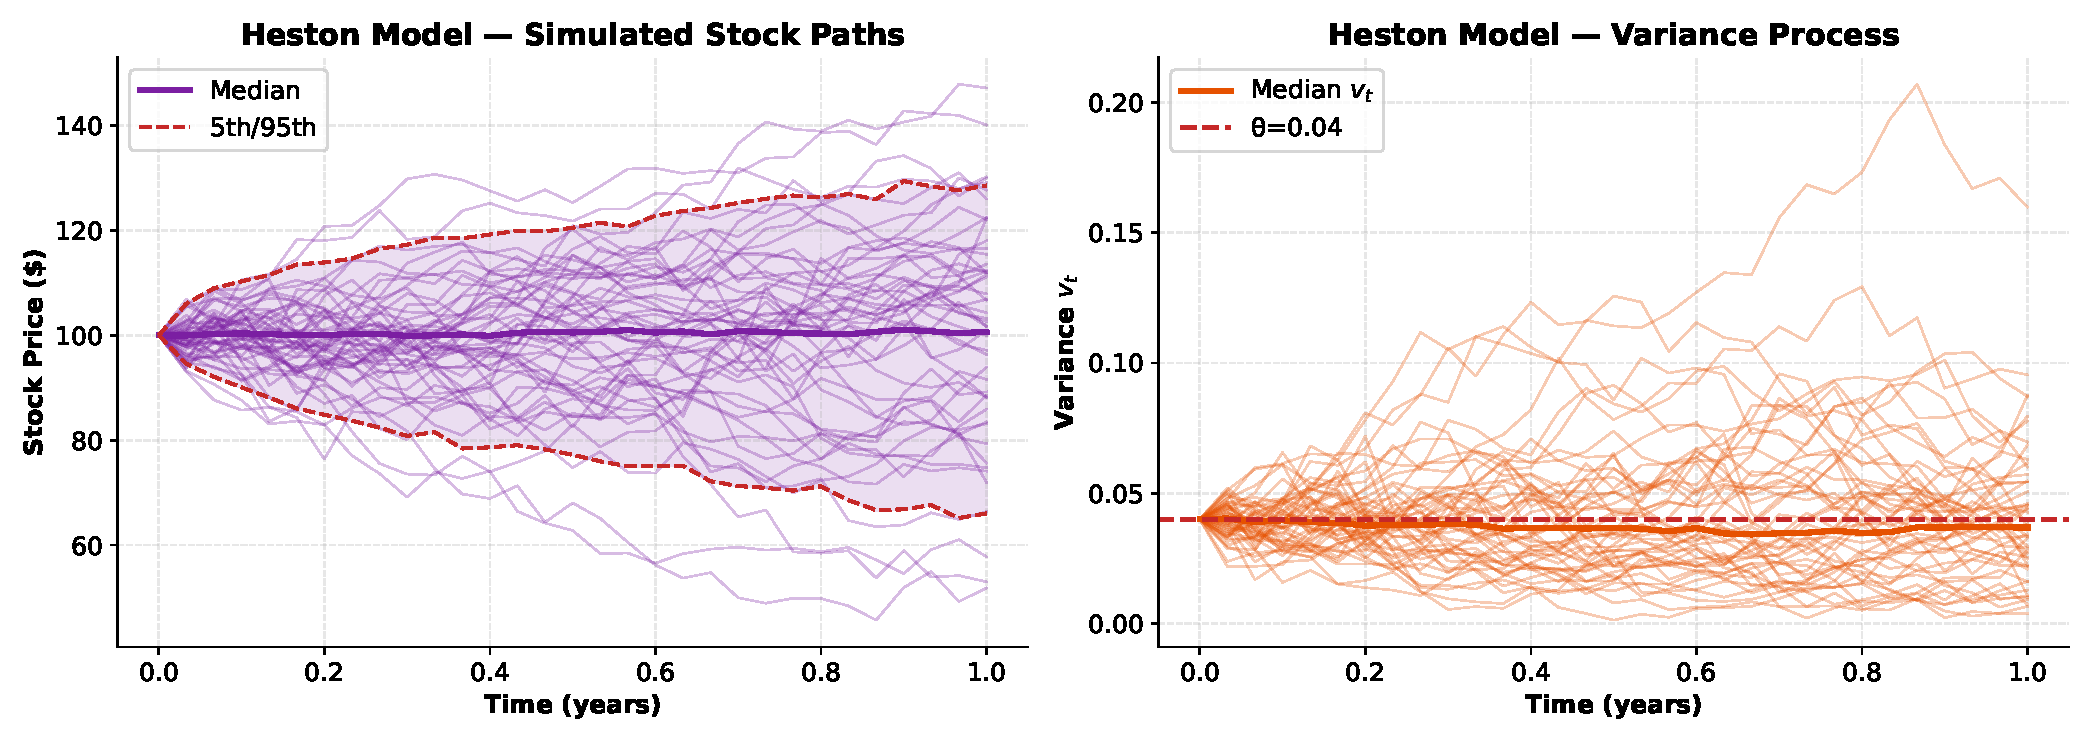
\includegraphics[width=0.88\textwidth]{figures/01_heston_stock_paths_and_variance.pdf}
\caption{Simulated Heston stock paths (left) and variance process (right) under the reference calibration of Table~\ref{tab:heston_params_setup}. The shaded band is the $5$th--$95$th percentile envelope across $5{,}000$ Monte-Carlo paths.}
\label{fig:heston_paths}
\end{figure}

\subsubsection{Model Parameters}

The reference calibration used in all in-distribution experiments is $S_0 = K = 100$, $v_0 = 0.04$,
$\kappa = 1.0$, $\theta_v = 0.04$, $\xi = 0.2$, $\rho = -0.7$, $r = 0.05$, $T = 30/365$, $N = 30$ 
(\textit{ATM setup; $20\%$ baseline volatility; moderate mean reversion; realistic vol-of-vol; leverage effect $\rho<0$; standard interest rate; 1-month maturity with daily rebalancing}). Crisis-regime calibrations (post-COVID, COVID, GFC 2008) raise the long-run variance and vol-of-vol parameters as detailed in Table~\ref{tab:heston_params_setup} and~\ref{tab:bates_calibrations}.


\begin{figure}[H]
\centering
  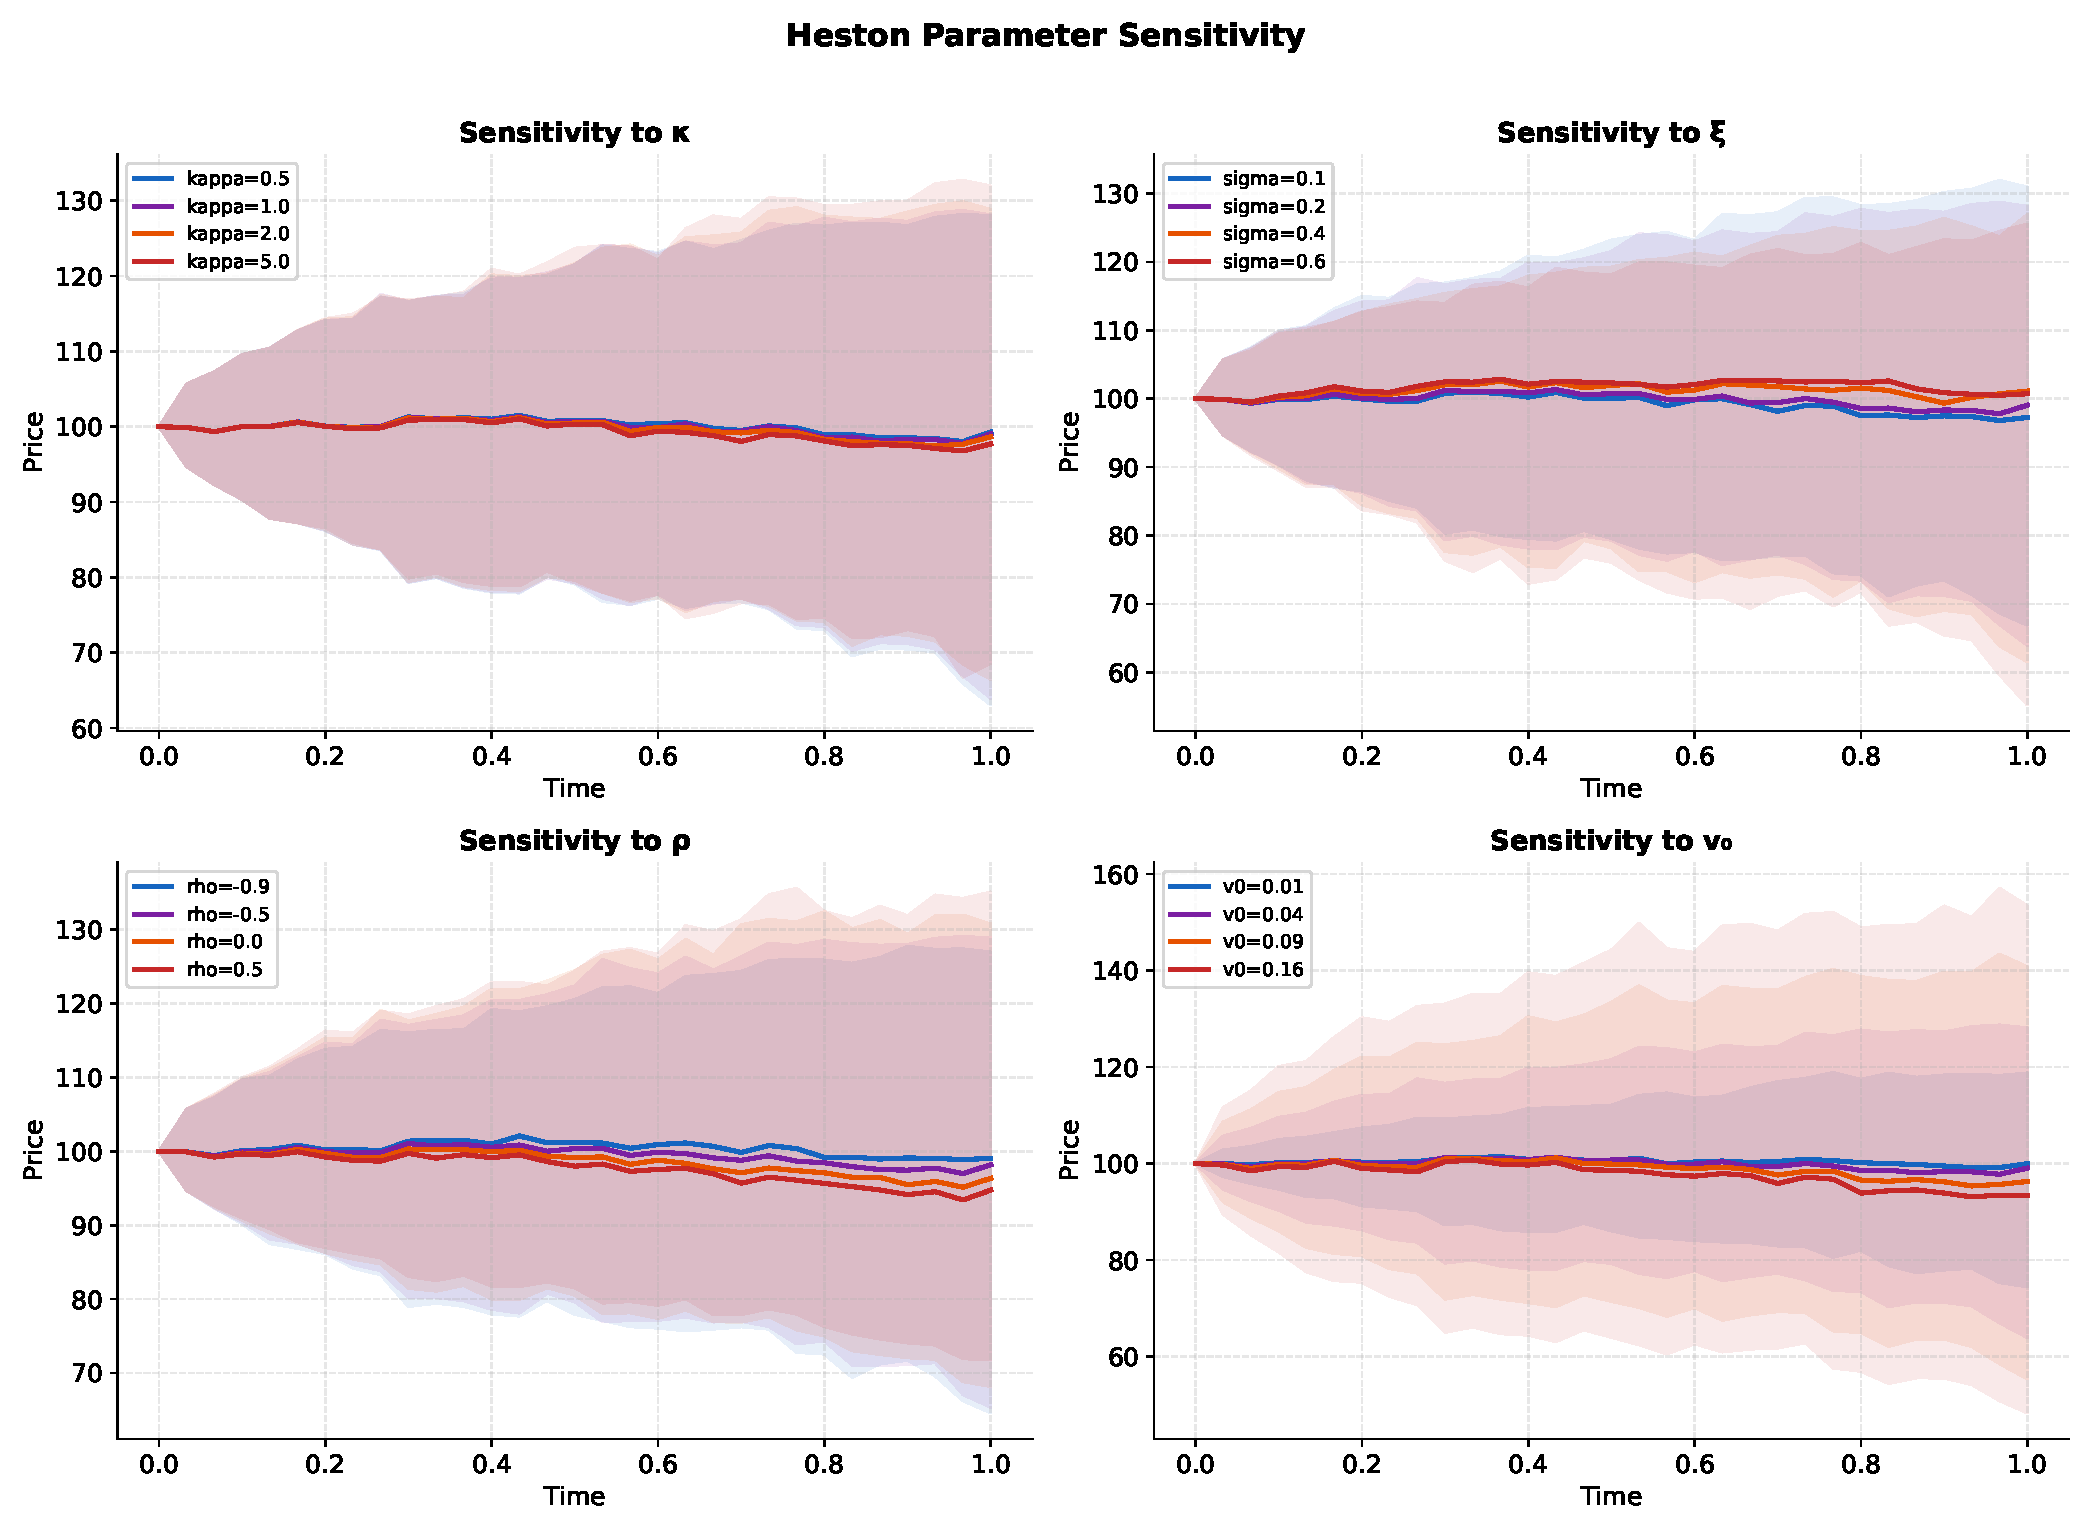
\includegraphics[width=0.77 \textwidth]{figures/03_heston_parameter_sensitivity.pdf}
\caption{Heston parameter sensitivity. Each panel sweeps one parameter --- mean-reversion speed $\kappa$, vol-of-vol $\xi$, leverage $\rho$ and initial variance $v_0$ --- holding the others at the reference calibration. The leverage panel shows the asymmetric response that motivates $\rho<0$ in the calibration.}
\label{fig:heston_sensitivity}
\end{figure}

% [INSERT FROM jaws_research/data/simulators.py + Bates 1996]
\subsubsection{Multi-Asset Bates Jump-Diffusion Extension}
\label{sec:bates}

Real index data show two features the pure Heston model cannot reproduce: discontinuous price moves on macroeconomic news days, and cross-asset correlations that tighten during stress. We extend the simulator to a multi-asset Bates jump-diffusion model so that the deep hedger sees both behaviours during training and evaluation.

Let $d\in\mathbb{N}$ index the basket assets and let $W_t^S = (W_t^{S,1},\ldots,W_t^{S,d})^\top$ be a $d$-dimensional Brownian motion with cross-asset correlation matrix $\Sigma\in\R^{d\times d}$ ($\Sigma_{ii}=1$, $\Sigma$ be symmetric positive semi-definite).  For each asset $i\in\{1,\ldots,d\}$ we add an independent compound Poisson jump term on top of the Heston diffusion:
\begin{align}
\frac{dS_t^i}{S_{t^-}^i} &= \bigl(r - \lambda_i\, m_J^i\bigr)\,dt + \sqrt{v_t^i}\, dW_t^{S,i} + \bigl(e^{J_t^i}-1\bigr)\,dN_t^i, \label{eq:bates_s}\\
dv_t^i &= \kappa_i\bigl(\theta_v^i - v_t^i\bigr)\,dt + \xi_i\sqrt{v_t^i}\, dW_t^{v,i}, \qquad
\langle W^{S,i},W^{v,i}\rangle = \rho_i\,dt, \label{eq:bates_v}
\end{align}
where $N^i\sim\mathrm{Poisson}(\lambda_i)$ counts jump arrivals, $J^i \stackrel{\text{i.i.d.}}{\sim} \mathcal{N}(\mu_J^i, (\sigma_J^i)^2)$ is the log-jump amplitude, and $m_J^i = \exp\!\bigl(\mu_J^i + (\sigma_J^i)^2/2\bigr)-1$ is the Bates jump compensator that keeps $S^i$ a martingale under the risk-neutral measure.  Cross-asset correlation $\Sigma$ is applied only to the diffusion innovations; jumps are independent across assets, which is consistent with empirical evidence that idiosyncratic jumps dominate single-asset news events~\citep{cont2001empirical}.

\begin{table}[H]
\centering\small
\caption{Regime-dependent jump and correlation parameters used in the Bates simulator.  Compounded with the Heston block parameters of Table~\ref{tab:heston_params_setup}.}
\label{tab:bates_calibrations}
\begin{tabular}{@{}lccccr@{}}
\toprule
\textbf{Regime} & $\lambda$ (per yr) & $\mu_J$ & $\sigma_J$ & cross-corr $\rho_{S}$ & $E[\#\text{jumps}/T]$ \\\midrule
Calm                & 1.5 & $-0.03$ & 0.10 & 0.55 & 0.12 \\
COVID-acute         & 6.0 & $-0.06$ & 0.18 & 0.75 & 0.49 \\
GFC 2008            & 8.0 & $-0.08$ & 0.22 & 0.75 & 0.66 \\
\bottomrule
\end{tabular}
\end{table}

The discretised Euler--Maruyama update follows~\eqref{eq:bates_s}--\eqref{eq:bates_v} with a full-truncation reflection on $v_{t}^i$ and a Poisson draw $N_k^i\sim\mathrm{Poisson}(\lambda_i\,\Delta t)$ at every step.  When $N_k^i\ge1$ the log-jump is the sum of $N_k^i$ i.i.d.\ Gaussians, which is itself a Gaussian with mean $N_k^i\,\mu_J^i$ and variance $N_k^i\,(\sigma_J^i)^2$.  Empirically, the typical $\lambda_i\Delta t$ at daily resolution is small enough that at most one jump per asset per step is observed, but the implementation does not require this approximation and supports compound jumps at coarser grids.

\section{Discretisation}

\subsubsection{Euler--Maruyama Scheme}

Full-truncation scheme on equidistant grid $\Delta t = T/N$:
\begin{align}
    S_{k+1} &= S_k \exp\!\bigl[(r - \tfrac{1}{2}v_k^+)\Delta t + \sqrt{v_k^+\Delta t}\;\epsilon_k^S\bigr], \\
    v_{k+1} &= v_k + \kappa(\theta_v - v_k)\Delta t + \xi\sqrt{v_k^+\Delta t}\;\epsilon_k^v,
\end{align}
where $v_k^+ = \max(v_k, 0)$ and $(\epsilon_k^S, \epsilon_k^v) \sim \mathcal{N}(0, \Sigma)$ with $\Sigma_{12} = \rho$.

\section{Deep Hedging Formulation}

\subsubsection{Hedging P\&L Definition}

For European call payoff $Z = (S_T - K)^+$ with $N = 30$ hedging steps:
\begin{equation}
    \mathrm{P\&L}(\delta) = -Z + \sum_{k=0}^{N-1} \delta_k (S_{t_{k+1}} - S_{t_k}) - c_{\mathrm{tc}} \sum_{k=0}^{N} |\delta_k - \delta_{k-1}| S_{t_k}
    \label{eq:pnl}
\end{equation}
with $c_{\mathrm{tc}} = 0.001$ and $\delta_{-1} = \delta_N = 0$ (flat entry/exit).

\subsubsection{Neural Policy Parameterisation}

$\theta^* = \argmin_\theta \rho(-\mathrm{P\&L}(\delta^\theta))$ with $\delta_k = \delta_{\max} \cdot \tanh(F_\theta(I_{0:k}, \delta_{k-1}))$, $\delta_{\max} = 1.5$.

\subsubsection{Feature Engineering}

$I_k = (S_k/S_0, \log(S_k/K), \sqrt{v_k}, \tau_k, \Delta_k^{\mathrm{BS}}) \in \R^5$ where $\tau_k = (T-t_k)/T$ is normalised time-to-maturity and $\Delta_k^{\mathrm{BS}}$ is Black--Scholes delta.

% [INSERT FROM jaws_research/tasks/payoffs.py]
\subsubsection{Exotic Payoffs and Hedge Sets}
\label{sec:tasks}

The published deep-hedging literature evaluates almost exclusively the at-the-money European call. The five hedgers in this thesis are tested on a wider set of payoffs so that no architecture can hide behind one that happens to suit its inductive bias. A hedging task is a tuple $(g, \mathcal{H})$ where $g:\R^{(N+1)\times d}\to\R$ is the terminal payoff and $\mathcal{H}\subseteq\{1,\ldots,d\}$ indexes the tradable hedge instruments. Unless stated otherwise, $K=100$ throughout.

\begin{table}[H]
\centering\small
\caption{Hedging-task suite used in the extended-suite benchmark of Chapter~\ref{sec:results} and Chapter~\ref{sec:crisis}.  $B$ is the barrier level, $C$ the digital coupon, and $w$ the basket weight vector.}
\label{tab:tasks}
\begin{tabular}{@{}lll@{}}
\toprule
\textbf{Name} & \textbf{Payoff $g$} & \textbf{Hedge set $\mathcal{H}$} \\\midrule
European call          & $(S_T-K)^+$                                                                & $\{S\}$ \\
European put           & $(K-S_T)^+$                                                                & $\{S\}$ \\
Up-and-out call ($B = 1.30K$)        & $(S_T-K)^+\cdot\mathbf{1}\{\max_{t\le T}S_t<B\}$            & $\{S\}$ \\
Down-and-in put  ($B = 0.80K$)        & $(K-S_T)^+\cdot\mathbf{1}\{\min_{t\le T}S_t<B\}$            & $\{S\}$ \\
Cash-or-nothing call   & $C\cdot \mathbf{1}\{S_T\ge K\}$, $C=10$                                    & $\{S\}$ \\
Asian call             & $\bigl(\frac{1}{N+1}\sum_{k=0}^N S_{t_k}-K\bigr)^+$                       & $\{S\}$ \\
Basket call ($d=3$)    & $\bigl(\langle w, S_T\rangle - K\bigr)^+,\quad w=(\tfrac13,\tfrac13,\tfrac13)$ & $\{S^1,S^2,S^3\}$ \\
\bottomrule
\end{tabular}
\end{table}

The barrier and digital payoffs are not differentiable in $S_T$, so the hedger cannot lean on a smooth Black--Scholes-style delta and must learn the discontinuity directly from path data. The Asian payoff depends on the entire path, which favours architectures with a path-aware backbone. The basket call is multi-asset: the hedge set contains all three underliers and the cross-asset correlation enters the optimal policy. The same payoff set is used in identical form across both the synthetic-Heston and real-data evaluations (Chapters~\ref{sec:results} and~\ref{sec:crisis}).

\section{Risk Measures}

\subsubsection{Conditional Value at Risk (CVaR)}

\begin{definition}[CVaR]
For loss $L = -\mathrm{P\&L}$ at level $\alpha \in (0,1)$:
\begin{align}
    \VaR_\alpha(L) &= \inf\{l \in \R : \PP(L \le l) \ge \alpha\}, \\
    \cvar_\alpha(L) &= \frac{1}{1-\alpha}\int_\alpha^1 \VaR_u(L)\,du = \E[L \mid L \geq \VaR_\alpha(L)].
\end{align}
CVaR is a coherent risk measure~\citep{artzner1999coherent}: monotonicity, translation invariance, positive homogeneity, and subadditivity.
\end{definition}
\begin{figure}[t]
\centering
\includegraphics[width=0.30\textwidth]{figures/cvar_plot.png}
\caption{Illustration of CVaR. The dashed line marks $\VaR_\alpha$, while the shaded region corresponds to tail losses whose conditional expectation defines $\cvar_\alpha$.}
\label{fig:cvar}
\end{figure}

\begin{proposition}[Rockafellar--Uryasev Dual~\citep{rockafellar2000optimization}]
\begin{equation}
    \cvar_\alpha(L) = \inf_{\nu \in \R}\Bigl\{\nu + \frac{1}{1-\alpha}\,\E\bigl[(L-\nu)^+\bigr]\Bigr\}.
\end{equation}
Differentiable in $\theta$ (a.e.), enabling gradient-based optimisation.
\end{proposition}

\subsubsection{Entropic Risk Measure}

\begin{definition}[Entropic Risk]
With risk aversion $\lambda > 0$:
\begin{equation}
    \rho_\lambda(X) = \frac{1}{\lambda}\log\E[\exp(-\lambda X)].
\end{equation}
Dual representation~\citep{follmer2002convex}: $\rho_\lambda(X) = \sup_{\QQ \ll \PP}\{\E_\QQ[-X] - \frac{1}{\lambda}\mathrm{KL}(\QQ\|\PP)\}$.
\end{definition}

\begin{remark}[CVaR vs.\ Entropic: Qualitative Differences]
CVaR focuses exclusively on the tail ($\alpha$-quantile and beyond), producing strategies that aggressively protect against worst-case losses but may over-trade. Entropic risk weighs all outcomes exponentially, producing smoother strategies.
\end{remark}

\subsubsection{Dual Representations of Risk Measures}

\begin{definition}[Generalised DRO Risk]
Given divergence $D(\QQ\|\PP)$ and radius $\varepsilon > 0$:
$\rho^D_\varepsilon(X) = \sup_{\QQ: D(\QQ\|\PP) \le \varepsilon} \E_\QQ[-X]$.
For $D = \mathrm{KL}$: entropic risk ($\varepsilon = 1/\lambda$). For $D = W_1$: Wasserstein DRO.
\end{definition}

\begin{remark}[Comparison of Ambiguity Sets]
\textbf{KL ball}: requires $\QQ \ll \PP$, adversary can only \emph{reweight} existing scenarios. \textbf{Wasserstein ball}: does \emph{not} require absolute continuity, adversary can \emph{move} mass to new regions. For crisis hedging, Wasserstein is more appropriate with distributional shifts like stress (COVID $\sigma = 65\%$) not seen during training ($\sigma \approx 20\%$).
\end{remark}

\begin{definition}[$1$-Wasserstein Distance]
For probability measures $\mu, \nu$ on $(\R^d, \|\cdot\|_2)$:
\begin{equation}
    W_1(\mu,\nu) = \inf_{\gamma \in \Gamma(\mu,\nu)} \int \|x-y\|_2\,d\gamma(x,y).
\end{equation}
Kantorovich--Rubinstein duality: $W_1(\mu,\nu) = \sup_{\|f\|_{\mathrm{Lip}} \le 1}\{\int f\,d\mu - \int f\,d\nu\}$.
\end{definition}


%%%%%%%%%%%%%%%%%%%%%%%%%%%%%%%%%%%%%%%%%%%%%%%%%%%%%%%%%%%%%%%%%%%%%%%%
% Part 2: Section 5 — Base and Novel Hedging Architectures
% (Poster Section 5: merges original Sections 5–8)
%%%%%%%%%%%%%%%%%%%%%%%%%%%%%%%%%%%%%%%%%%%%%%%%%%%%%%%%%%%%%%%%%%%%%%%%

\chapter{Base and Novel Hedging Architectures}
\label{sec:architectures}

\section{Base Hedging Architectures}
\label{sec:base}

\subsubsection{LSTM Hedger Architecture}

Our LSTM baseline follows the recurrent specification adopted in~\citet{buehler2019deep}, which has become the reference deep-hedging architecture in the post-2019 literature.

\begin{definition}[LSTM Hedger]
The LSTM hedger processes the feature sequence $(I_0, \dots, I_k)$ through a multi-layer LSTM:

\begin{align}
h_k, c_k &= \mathrm{LSTM}([I_k; \delta_{k-1}],\, h_{k-1}, c_{k-1}) \label{eq:lstm_state} \\
\delta_k &= \delta_{\max} \cdot \tanh(W_o h_k + b_o) \label{eq:lstm_output}
\end{align}

where $[I_k; \delta_{k-1}]$ denotes concatenation, and $(h_k, c_k)$ are the hidden and cell states.
\end{definition}

\paragraph{Architecture details.}
We use a 2-layer LSTM with hidden dimension 50, followed by a linear output layer.

\vspace{0.5em}

\subsubsection{AttentionLSTM Architecture}

We augment the LSTM with a temporal attention mechanism to capture long-range dependencies.

\begin{definition}[AttentionLSTM]
The AttentionLSTM computes attention weights over the sequence of hidden states:

\begin{align}
\alpha_{k,j} &= 
\frac{\exp\left(h_k^\top W_a h_j\right)}
{\sum_{i=0}^{k} \exp\left(h_k^\top W_a h_i\right)} \label{eq:attention_weights} \\
c_k^{\mathrm{attn}} &= \sum_{j=0}^{k} \alpha_{k,j} h_j \label{eq:attention_context} \\
\delta_k &= \delta_{\max} \cdot \tanh\left(W_o [h_k; c_k^{\mathrm{attn}}] + b_o\right) \label{eq:attention_output}
\end{align}

This architecture allows the model to directly access any past hidden state, improving its ability to model long-range temporal dependencies compared to vanilla LSTM.
\end{definition}

\vspace{0.5em}

\subsubsection{Transformer Hedger Architecture}

We adapt the Transformer encoder architecture of \citet{vaswani2017attention} for hedging.

\begin{definition}[Transformer Hedger]
The Transformer hedger processes features using self-attention with causal masking:

\begin{align}
X_0 &= \mathrm{InputProjection}([I_0; 0], \dots, [I_k; \delta_{k-1}]) + \mathrm{PE} \label{eq:transformer_input} \\
X_l &= \mathrm{TransformerLayer}(X_{l-1}, \mathrm{CausalMask}), \quad l = 1, \dots, L \label{eq:transformer_layers} \\
\delta_k &= \delta_{\max} \cdot \tanh\big(\mathrm{OutputHead}(X_L[k])\big) \label{eq:transformer_output}
\end{align}

where $\mathrm{PE}$ denotes sinusoidal positional encoding and $\mathrm{CausalMask}$ prevents attention to future time steps.
\end{definition}

\paragraph{Architecture details.}
We use $d_{\text{model}} = 64$, $n_{\text{heads}} = 4$, $n_{\text{layers}} = 3$, $d_{\text{ff}} = 256$, and GELU activation.

\subsubsection{Signature-Based Hedger}

Path signatures~\citep{lyons1998differential}: $\mathrm{Sig}(X)_{[s,t]} = (1, \int_s^t dX_u, \int_s^t\int_s^u dX_v dX_u, \ldots)$ truncated at depth $m$. Captures order of events, oscillation patterns, roughness, and non-Markovian effects. Running statistics (mean $\mu_t$, std $\sigma_t$, max/min) of signature features are fed to an MLP producing path-dependent hedge ratios. Used as frozen base model within RSE.

\section{Regime-Switching Ensemble (RSE)}
\label{sec:rse}

\subsubsection{Ensemble Variance Reduction Theory}

Classical ensemble theory~\citep{dietterich2000ensemble} shows that combining $M$ diverse models reduces variance. For equal-weight averaging:
\begin{equation}
    \mathrm{Var}(\bar{f}) = \frac{\bar\sigma^2}{M} + \frac{M-1}{M}\,\bar\rho\,\bar\sigma^2
    \label{eq:ensemble_classical}
\end{equation}
where $\bar{\rho}$ is average pairwise correlation and $\bar\sigma^2$ is average individual variance. When $\bar\rho < 1$, the ensemble variance is strictly less than the average individual variance, with improvement proportional to model diversity ($1-\bar\rho$).

\subsubsection{RSE Architecture Overview}

RSE consists of four components operating in sequence:

\begin{definition}[Regime-Switching Ensemble]
The ensemble delta at time step $k$ is:
\begin{equation}
    \delta_k^{\mathrm{RSE}} = \sum_{m=1}^{M} w_m(r_k) \cdot \delta_k^{(m)}
    \label{eq:rse}
\end{equation}
where $\delta_k^{(m)}$ are base model outputs, $r_k$ is the detected regime label, and $w_m(r_k) = \sum_{j=1}^K p(r_k = j) \cdot [\mathrm{softmax}(A)]_{j,m}$ are regime-dependent model weights derived from the gating network.
\end{definition}

\subsubsection{Regime Feature Extraction}

We extract six regime-relevant and market microstructure features from price paths:

\begin{definition}[Regime Features]
At time step $k$, the regime feature vector is:
\begin{equation}
    x_k^{\mathrm{reg}} = \bigl(\mathrm{RV}_k^{(5)},\; \mathrm{RV}_k^{(10)},\; \mathrm{RV}_k^{(20)},\; \mathrm{Trend}_k,\; \mathrm{Mom}_k,\; \mathrm{Jump}_k\bigr)
\end{equation}
\end{definition}

\textbf{Realized Volatility} at windows $w \in \{5, 10, 20\}$:
\begin{equation}
    \mathrm{RV}_k^{(w)} = \sqrt{\frac{1}{w} \sum_{i=k-w+1}^{k} (\log S_i - \log S_{i-1})^2}
\end{equation}

\textbf{Trend Indicator} (SMA crossover):
\begin{equation}
    \mathrm{Trend}_k = \frac{\mathrm{SMA}_5(S_k) - \mathrm{SMA}_{20}(S_k)}{\mathrm{SMA}_{20}(S_k)}
\end{equation}

\textbf{Momentum:}
\begin{equation}
    \mathrm{Mom}_k = \frac{S_k - S_{k-5}}{S_{k-5}}
\end{equation}

\textbf{Jump Indicator} (Barndorff-Nielsen ratio):
\begin{equation}
    \mathrm{Jump}_k = \frac{\mathrm{RV}_k^{(20)}}{\mathrm{BV}_k^{(20)}}
\end{equation}
where $\mathrm{BV}_k^{(w)} = \frac{\pi}{2} \sum_{i} |u_i| \cdot |u_{i+1}|$ is bipower variation, with $u_i = \log S_i - \log S_{i-1}$, and $\mathrm{Jump} > 1$ indicates jump activity.

\begin{figure}[H]
\centering
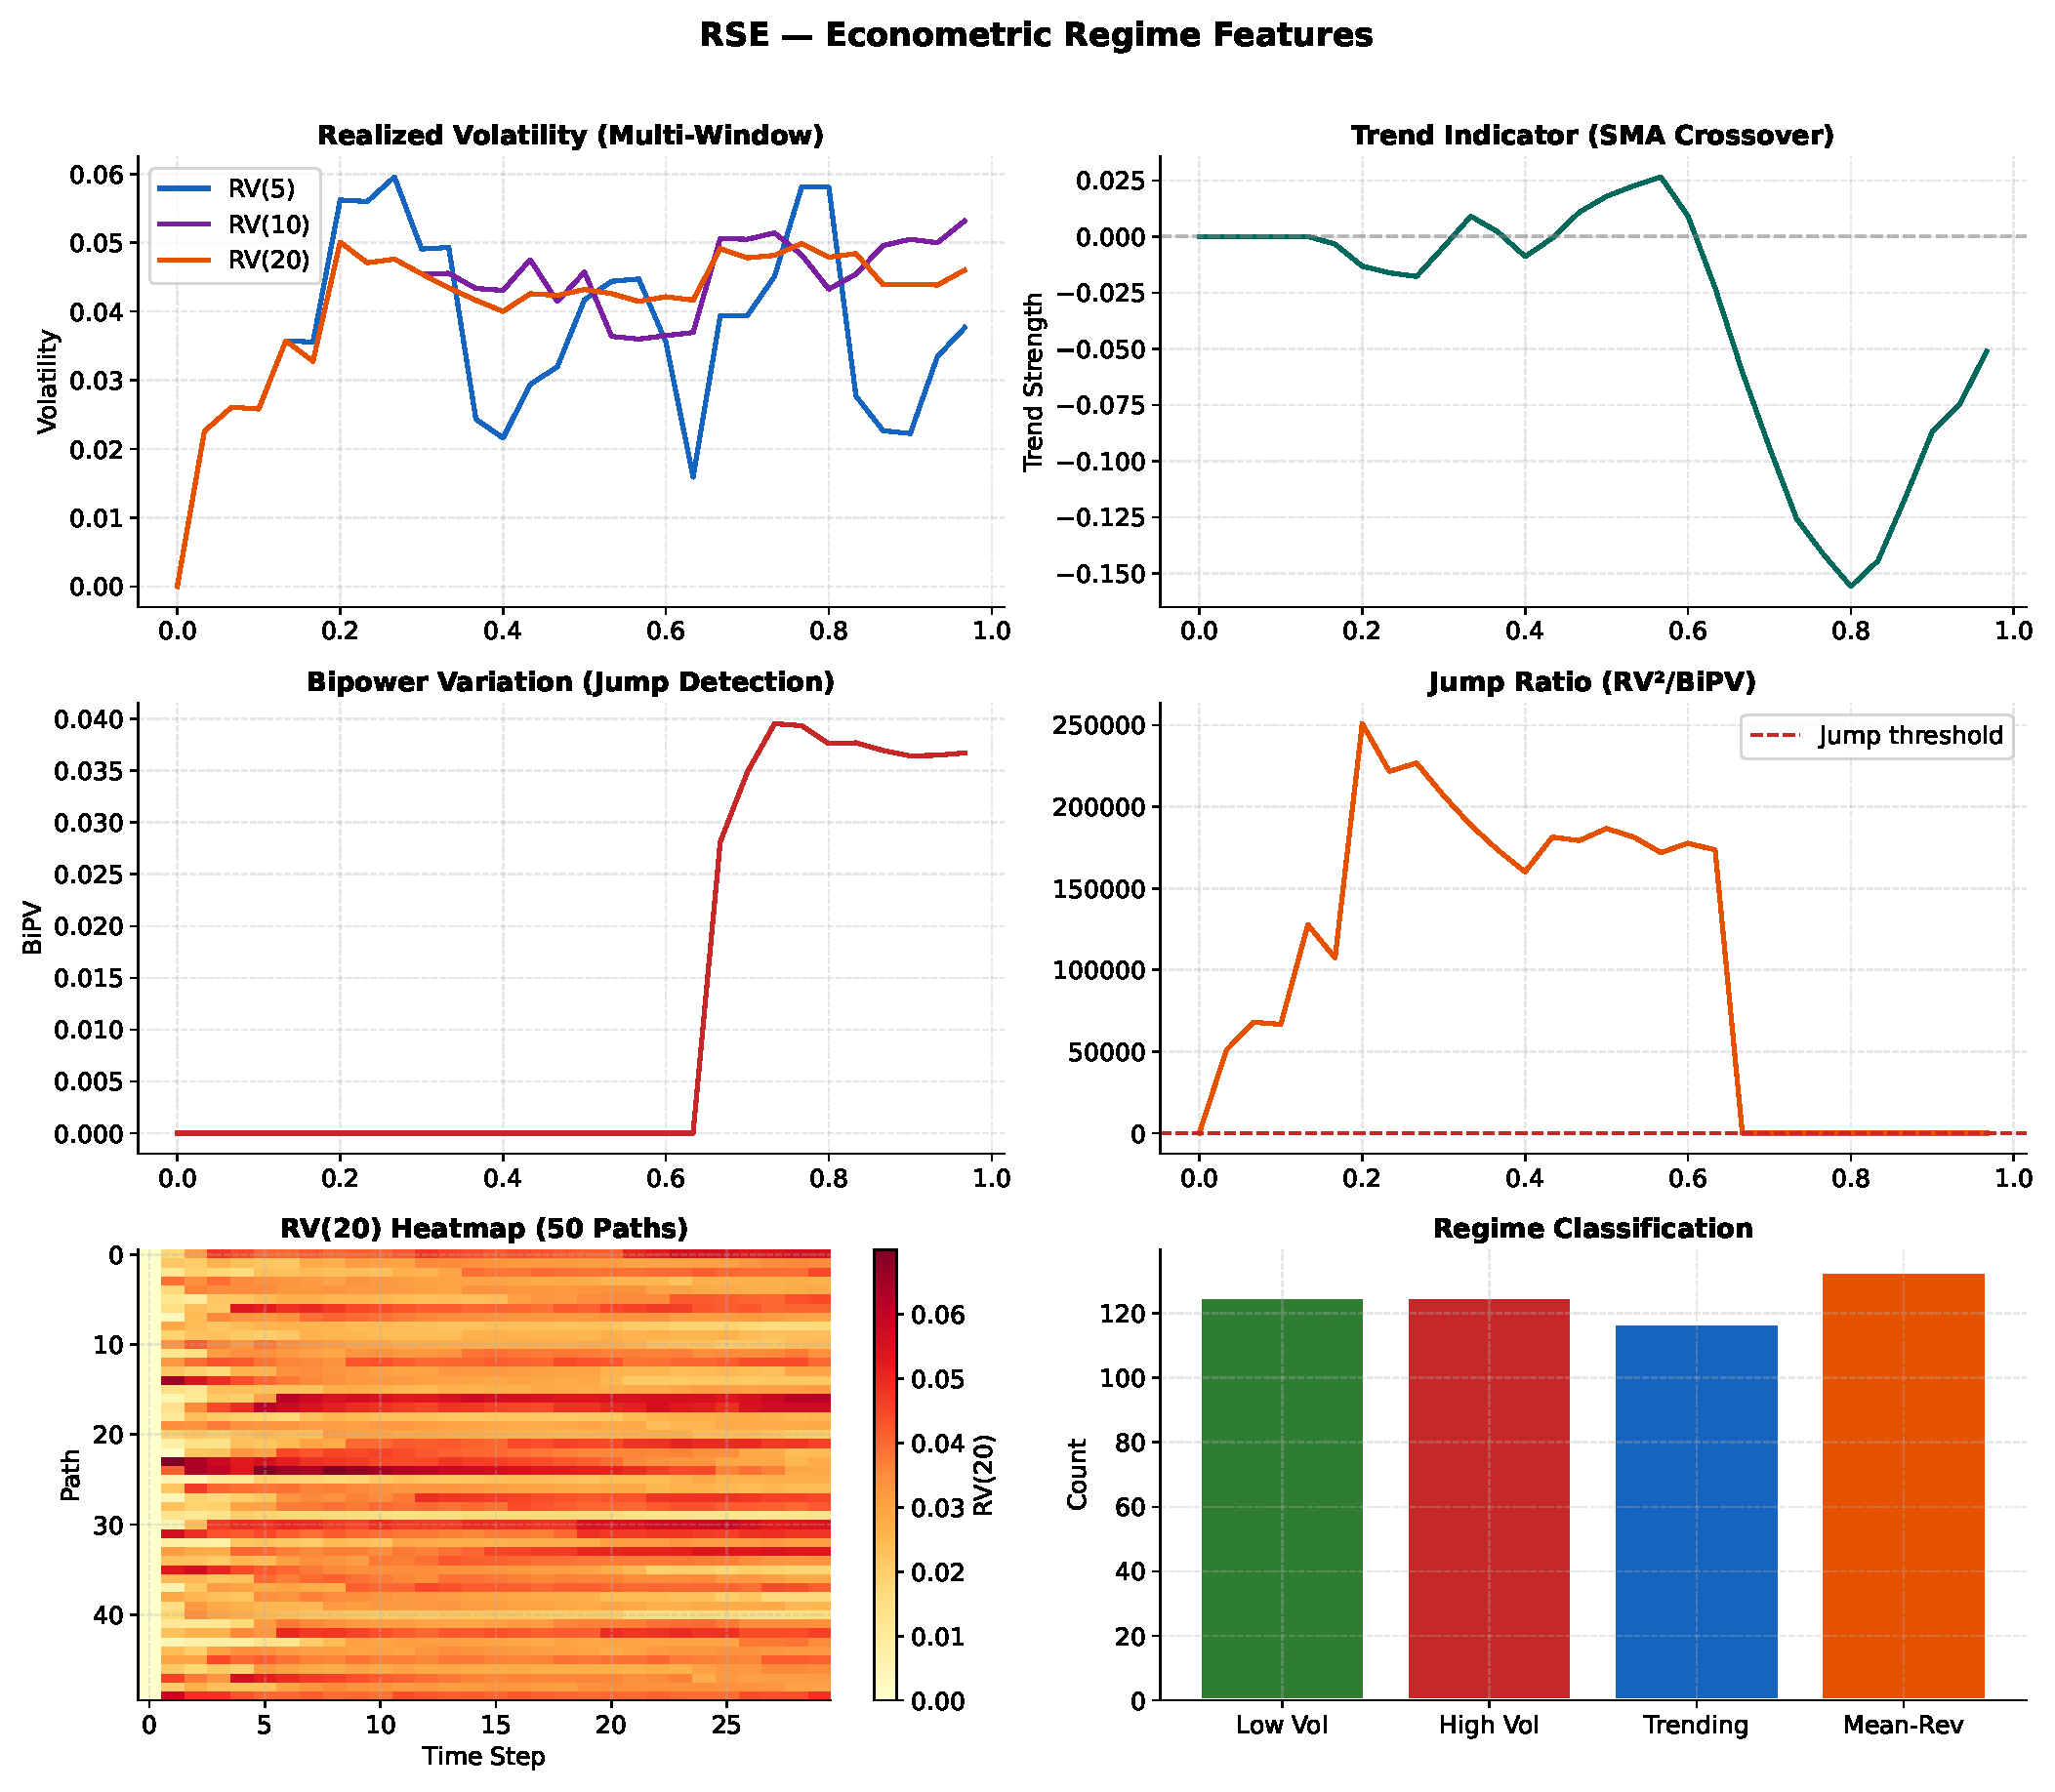
\includegraphics[width=0.88\textwidth]{figures/13_rse_regime_features.pdf}
\caption{RSE regime features along a representative simulated path: multi-window realised volatility, the SMA-crossover trend indicator, bipower variation and the jump ratio. These are the inputs the regime classifier $f_\phi$ consumes at every time step.}
\label{fig:rse_regime_features}
\end{figure}

\subsubsection{Regime Classifier}

An MLP maps features to $K = 4$ regime probabilities:
\begin{equation}
    p(r_k = j \mid I_{0:k}) = \mathrm{softmax}\bigl(f_\phi(x_k^{\mathrm{reg}})\bigr)_j
\end{equation}
where $f_\phi$ is a 3-layer network: $\R^6 \to \R^{64} \to \R^{64} \to \R^4$ with ReLU activations and batch normalization.

The four regimes correspond approximately to: (1) Low volatility / calm, (2) High volatility / stressed, (3) Trending, (4) Mean-reverting / choppy.

\subsubsection{Regime-Dependent Gating Network}

A learnable affinity matrix $A \in \R^{K \times M}$ maps regimes to model weights:
\begin{equation}
    w_m(k) = \sum_{j=1}^{K} p(r_k = j) \cdot \underbrace{[\mathrm{softmax}(A/\tau)]_{j,m}}_{\text{regime-to-model affinity}}
    \label{eq:gating}
\end{equation}
where $\tau > 0$ is the softmax temperature (set to $\tau = 1$ in our experiments).  The softmax over columns ensures that weights sum to 1 across models for each regime.  The affinity matrix $A$ is the key learnable component: it encodes which base model is best for each regime.

\begin{remark}[Softmax Temperature and Gating Sharpness]
The temperature $\tau$ controls the sharpness of the gating distribution:
\begin{itemize}[noitemsep]
    \item As $\tau \to 0^+$, $\mathrm{softmax}(A/\tau) \to$ one-hot (hard switching between models).
    \item As $\tau \to \infty$, $\mathrm{softmax}(A/\tau) \to \mathbf{1}/M$ (uniform equal weighting).
\end{itemize}
With $\tau = 1$, the learned affinity matrix (Table~\ref{tab:affinity}) shows weights ranging from 0.18 to 0.54, indicating soft blending rather than hard switching.  Soft gating is preferable for hedging to avoid discontinuous strategy changes at regime boundaries, which would generate unnecessary transaction costs.
\end{remark}

\subsubsection{Training Protocol}
\begin{algorithm}[htbp]
\caption{RSE Training Protocol}
\label{alg:rse}
\begin{algorithmic}[1]
\REQUIRE Data $\mathcal{D}$, base model architectures
\STATE \textbf{Step 1: Pre-train base models} (30 epochs each)
\FOR{$m \in \{\text{LSTM, Trans., Sig.}\}$}
    \STATE Train $F_{\theta_m}$ with $\cvar_{0.95}$ loss
    \STATE Freeze: $\theta_m \gets \text{const}$
\ENDFOR
\STATE
\STATE \textbf{Step 2: Train gating (CVaR)} (20 epochs)
\STATE Trainable params: $\phi$ (classifier), $A$ (affinity)
\FOR{epoch $= 1$ to 20}
    \FOR{batch $(I, S, Z) \sim \mathcal{D}$}
        \STATE $\delta^{\mathrm{RSE}} \gets \sum_m w_m(r) \cdot F_{\theta_m}(I)$ \hfill Eq.~\eqref{eq:rse}
        \STATE $\mathcal{L} \gets \cvar_{0.95}(-\mathrm{P\&L})$
        \STATE Update $\phi, A$ via Adam (lr $= 10^{-3}$)
    \ENDFOR
\ENDFOR
\STATE
\STATE \textbf{Step 3: Fine-tune gating (Entropic)} (30 epochs)
\FOR{epoch $= 1$ to 30}
    \FOR{batch $(I, S, Z) \sim \mathcal{D}$}
        \STATE $\mathcal{L} \gets \rho_\lambda(-\mathrm{P\&L})$
        \STATE Update $\phi, A$ via Adam (lr $= 10^{-4}$)
    \ENDFOR
\ENDFOR
\RETURN $\phi^*, A^*$
\end{algorithmic}
\end{algorithm}
\noindent\textbf{Training budget.} 
$3 \times 30 + 20 + 30 = 140$ model-epochs ($\approx 80$ single-model equivalent).

\subsubsection{Regime--Model Affinity Matrix}

\begin{table}[]\centering\small
\caption{Learned affinity (typical run, after softmax).}\label{tab:affinity}
\begin{tabular}{lccc}\toprule
\textbf{Regime} & \textbf{LSTM} & \textbf{Transformer} & \textbf{Signature} \\\midrule
Low vol (calm) & \textbf{0.52} & 0.28 & 0.20 \\
High vol (stress) & 0.18 & \textbf{0.54} & 0.28 \\
Trending & 0.31 & \textbf{0.41} & 0.28 \\
Mean-reverting & \textbf{0.45} & 0.22 & 0.33 \\
\bottomrule
\end{tabular}
\end{table}

LSTM dominates calm/mean-reverting regimes; Transformer dominates high-vol/trending; Signature provides consistent 20--33\% weight (path-dependent regularisation). This interpretability supports model risk governance.

\subsubsection{Complexity and Interpretability}

Per-step complexity is $\mathcal{O}(M\,C_{\max} + C_{\text{gate}})$ with $C_{\max}=\mathcal{O}(N^2 d^2)$ for the dominant Transformer base; the affinity matrix carries only $KM = 12$ trainable scalars and the gating classifier $f_\phi$ has fewer than $5$K parameters.  Inference latency is $<10$~ms on a parallel GPU.  RSE exposes a three-level audit trail at zero retraining cost: (i)~the time-varying regime probabilities $p(r_k=j)$ output by $f_\phi$; (ii)~the time-varying model weights $w_m(r_k)$ that attribute the ensemble action to each base hedger; and (iii)~the static affinity matrix $A$ of Table~\ref{tab:affinity}, auditable offline.  Three graceful rollback levels are available ie. set $w_m \equiv 1/M$ for equal-weight averaging, select the single best base model per regime, or revert to LSTM; none of which requires retraining.  
\subsubsection{Regime Classification Model Validation}

Validated via: (1) high-vol regime probability correlates with RV ($\rho > 0.7$); (2) trend probability correlates with SMA crossover ($\rho > 0.5$); (3) temporally smooth transitions.
\subsubsection{Ablation: Number of Base Models}

\begin{table}[H]
\centering
\caption{Ablation: number of base models}
\label{tab:ablation_models}
\small
\begin{tabular}{lccc}
\toprule
\textbf{Ensemble} & \textbf{CVaR$_{95}$} & \textbf{CV\%} & \textbf{$\Delta$ vs.\ Full} \\
\midrule
LSTM only & 3.215 & 0.55 & $+3.4\%$ \\
LSTM + Transformer & 3.142 & 0.38 & $+1.1\%$ \\
\textbf{Full (3 models)} & \textbf{3.109} & \textbf{0.30} & --- \\
\bottomrule
\end{tabular}
\end{table}

Each additional expert yields diminishing but consistent CVaR improvement, with the Signature model providing the final $1.1\%$ gain.


\subsubsection{Ablation: Number of Regimes}

\begin{table}[htbp]
\centering
\caption{Ablation: number of regimes $K$}
\label{tab:ablation_regimes}
\small
\begin{tabular}{lcc}
\toprule
\textbf{$K$} & \textbf{CVaR$_{95}$} & \textbf{Interpretation} \\
\midrule
2 & 3.128 & Under-specified \\
3 & 3.115 & Competitive \\
\textbf{4 (default)} & \textbf{3.109} & Optimal \\
6 & 3.112 & Diminishing returns \\
\bottomrule
\end{tabular}
\end{table}

The optimal choice is $K=4$, balancing expressivity and parameter efficiency.


\section{Three-Stage Curriculum Hedger (3SCH)}
\label{sec:3sch}

\subsubsection{Motivation and Curriculum-Learning Perspective}

The two-stage \citet{kozyra2019deep} protocol switches abruptly from $\cvar_{0.95}$ to $\rho_\lambda$ between Stage~1 and Stage~2, which produces gradient discontinuities, occasional forgetting of the tail-aware solution, and convergence to local minima. In the curriculum-learning view of~\citet{bengio2009curriculum}, CVaR is the easier tail-focused objective and entropic is the harder global one. We replace the abrupt switch with a homotopy whose regularity is provable. Specifically, we use the convex combination
\begin{equation}
    \mathcal{L}_{\mathrm{mixed}}(\alpha; \theta) = \alpha \cdot \cvar_{0.95}(-\mathrm{P\&L}^\theta) + (1-\alpha) \cdot \rho_\lambda(-\mathrm{P\&L}^\theta)
\end{equation}
which is a convex risk measure for each fixed $\alpha$ and a scalarisation of the underlying bi-objective problem. Berge's maximum theorem~\cite{berge1963topological,aliprantis2006infinite} (Appendix~\ref{app:theory}) gives upper hemicontinuity of $\alpha\mapsto\Theta^*(\alpha)$, which justifies the homotopy continuation. 3SCH inherits the LSTM architecture (two layers, $h=50$, around 54K parameters) without modification, so any improvement is attributable to the schedule rather than the capacity.

\subsubsection{Annealing Schedule and Three-Stage Protocol}

We anneal $\alpha(t) = 0.8 - 0.6\,t/(T_2-1)$ for $t=0,\ldots,T_2-1$.  The starting value $0.8$ retains a $20\%$ entropic gradient signal from the first homotopy epoch, and the terminal value $0.2$ keeps a CVaR regulariser before Stage~3 takes over.

\begin{algorithm}[H]
\caption{Three-Stage Curriculum Hedger (3SCH)}
\begin{algorithmic}[1]
\STATE \textbf{Stage 1} ($T_1 = 40$ ep): $\mathcal{L} = \cvar_{0.95}$, lr $= 10^{-3}$, patience 15
\STATE Store reference deltas $\delta^{\text{ref}} \gets F_\theta(I)$
\STATE \textbf{Stage 2} ($T_2 = 15$ ep): $\alpha$ anneals $0.8 \to 0.2$, lr $= 5 \times 10^{-4}$
\FOR{epoch $= 1$ to $T_2$}
    \STATE $\alpha \gets 0.8 - 0.6(t-1)/(T_2 - 1)$
    \STATE $\mathcal{L} \gets \alpha \cdot \cvar_{0.95} + (1-\alpha) \cdot \rho_\lambda$
\ENDFOR
\STATE \textbf{Stage 3} ($T_3 = 25$ ep): $\mathcal{L} = \rho_\lambda + \gamma|\Delta\delta|$, lr $= 10^{-4}$, patience 10
\RETURN $\theta^*$
\end{algorithmic}
\end{algorithm}

\begin{figure}[]
\centering
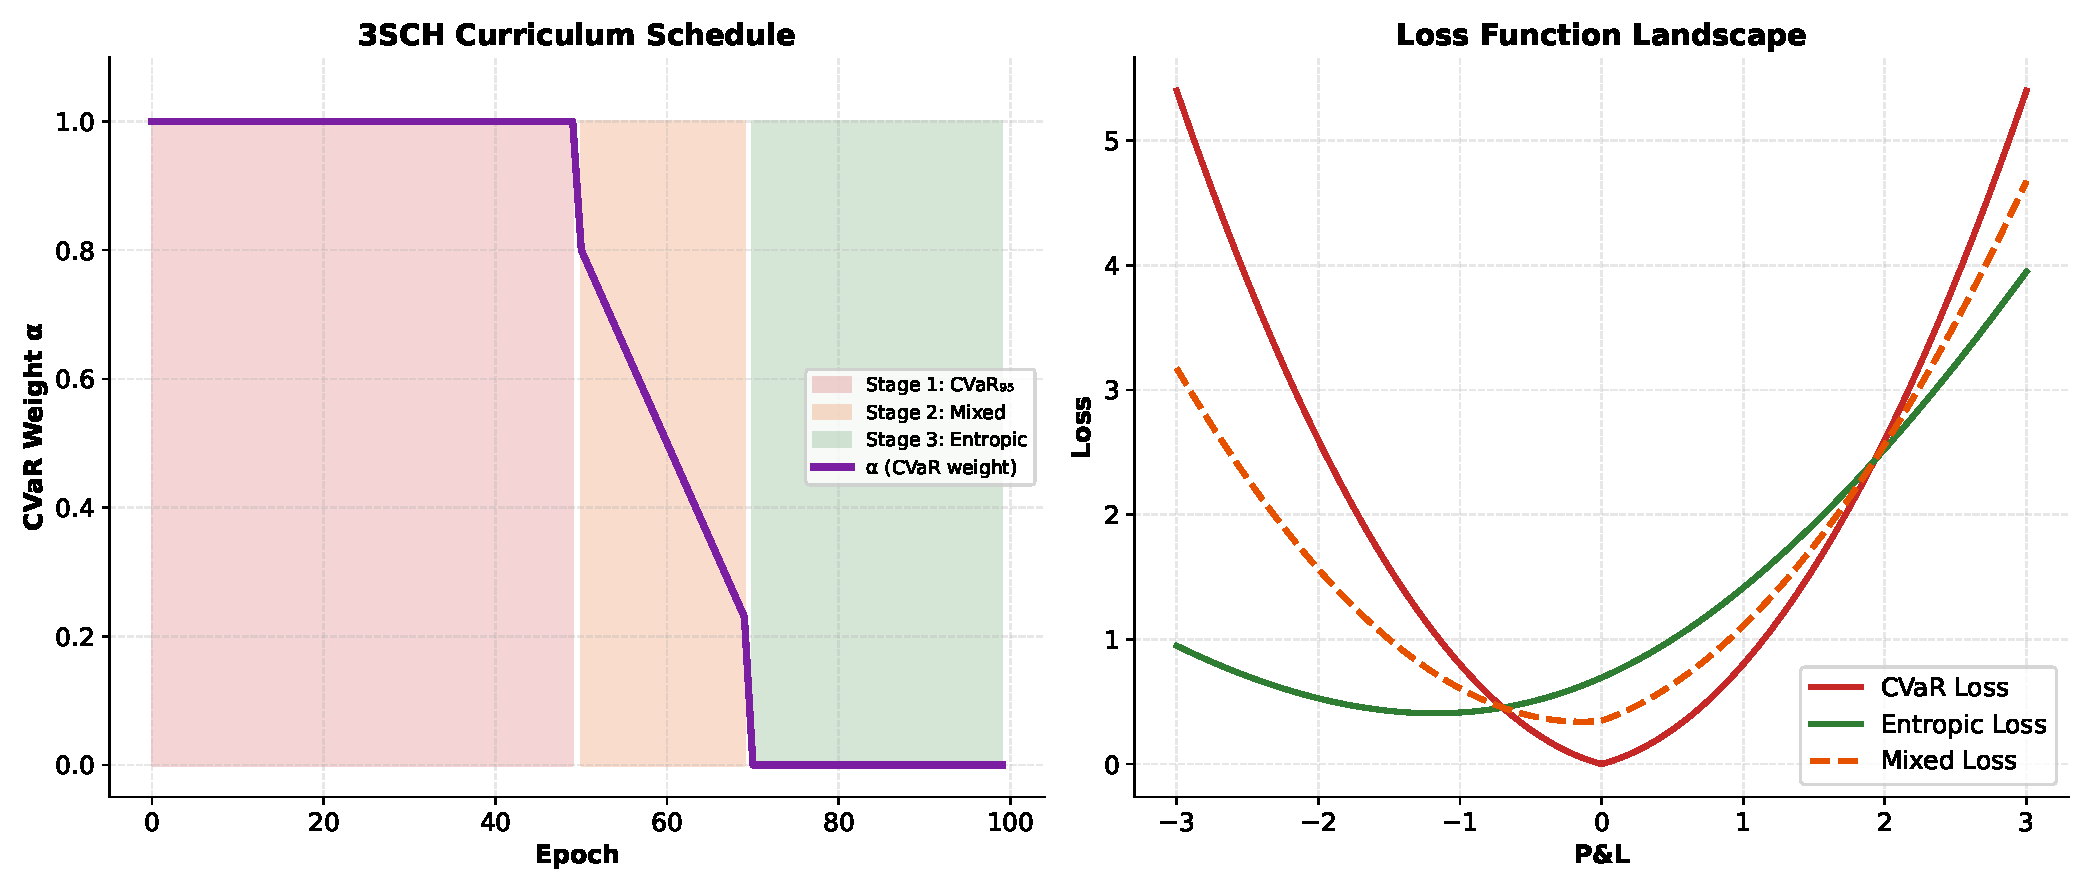
\includegraphics[width=0.75\textwidth]{figures/17_training_schedule_3sch.pdf}
\caption{Left: 3SCH curriculum schedule. The CVaR weight $\alpha$ is held at $1$ during Stage~1, anneals from $0.8$ to $0.2$ across Stage~2, and drops to $0$ in Stage~3. Right: the corresponding loss-function landscape at three representative weights, showing the smooth deformation between the CVaR and entropic objectives.}
\label{fig:3sch_schedule}
\end{figure}

\textbf{Total:} 80 epochs, matching the fair two-stage budget; the homotopy transition is absorbed into the shared budget rather than added on top.  Stage~3 adds two soft constraints: a trading penalty $\mathrm{TP}(\delta) = \gamma\sum_k|\delta_k-\delta_{k-1}|$ with $\gamma=10^{-3}$, and a no-trade band penalty $\mathrm{BP}(\delta) = \nu\sum_k\max(0,|\delta_k-\delta_k^{\mathrm{ref}}|-\epsilon)$ with $\nu=10^8$, $\epsilon=0.15$.  The band penalty discourages large deviations from the CVaR-optimal Stage-1 reference deltas $\delta^{\mathrm{ref}}$, which empirically prevents catastrophic forgetting of tail-aware behaviour during the entropic stage.  Per-seed training time is $\sim 295$~s and the additional space cost is the cached $\delta^{\mathrm{ref}}$. 

\section{Wasserstein DRO Transformer (W-DRO-T)}
\label{sec:wdrot}

\subsubsection{Distributional Shift and DRO Formulation}

Heston-trained policies degrade more than four-fold in $\cvar_{95}$ when deployed under COVID-style volatility ($\sigma\approx65\%$) they were never trained on. W-DRO-T narrows this gap by minimising worst-case risk over a Wasserstein ball~\citep{esfahani2018data} around the training measure:
\begin{equation}
\theta^* = \argmin_\theta \sup_{\QQ:\,W_p(\QQ,\PP)\le\varepsilon}
\E_\QQ\bigl[\rho(\mathrm{P\&L}(\delta^\theta))\bigr],
\label{eq:dro_obj}
\end{equation}
with ambiguity set $\mathcal{P}^W(\PP;\varepsilon) = \{\QQ:W_p(\QQ,\PP)\le\varepsilon\}$ and radius $\varepsilon>0$. Unlike the KL ball implicit in entropic risk, which only re-weights existing scenarios because it requires $\QQ\ll\PP$, the Wasserstein ball can \emph{move} probability mass to new regions of the input space and therefore bounds risk under support shifts such as a regime change in volatility~\citep{esfahani2018data}.

\subsubsection{Tractable Dual and Gradient-Norm Penalty}

The supremum in~\eqref{eq:dro_obj} is intractable in general. Strong duality~\citep{esfahani2018data,blanchet2019quantifying} yields the equivalent dual formulation
\begin{equation}
\sup_{W_1(\QQ,\PP)\le\varepsilon} \E_\QQ[\ell]
=
\inf_{\lambda\ge0}
\left\{
\lambda\varepsilon + \E_\PP\!\left[
\sup_{x'}\{\ell(x') - \lambda\|x-x'\|\}
\right]
\right\},
\end{equation}
which corresponds to the Kantorovich dual (or $c$-transform).

A first-order expansion in $\varepsilon$ yields the practical training objective:
\begin{corollary}[Gradient-Penalty Approximation]
\label{cor:grad_penalty}
\begin{equation}
\mathcal{L}_{\mathrm{DRO}}(\theta)
=
\E_\PP[\ell(\theta;X)]
+
\varepsilon\,\E_\PP[\|\nabla_X \ell(\theta;X)\|_2]
+
O(\varepsilon^2),
\label{eq:dro_loss}
\end{equation}
\end{corollary}
valid under smoothness and local Lipschitz assumptions on $\ell$.

The resulting penalty controls input sensitivity in the spirit of a Lipschitz constraint and is optimisation-friendly: unlike the density-ratio penalty induced by a KL ambiguity set, it remains stable for the small radii used in our annealing schedule.
\paragraph{Architecture and second-order gradient.}
W-DRO-T inherits the causal Transformer of Section~\ref{sec:base} ($d_{\mathrm{model}}=64$, $H=4$, $L=3$, $d_{\mathrm{ff}}=256$, dropout $0.1$, $\sim$85K parameters).  Because the ~\eqref{eq:dro_loss} is a function of $\theta$ through the full chain rule (Appendix~\ref{app:theory}), optimising~\eqref{eq:dro_loss} requires second-order gradients via \texttt{torch.autograd.grad(\dots,create\_graph=True)}.  The fused efficient/flash SDPA kernels do not support this, so we force the MATH backend during DRO training; the cost is roughly a doubling of per-batch wall time in Stage~2 and zero overhead at inference.


\subsubsection{Three-Phase Training Protocol}

\begin{algorithm}[htbp]
\caption{W-DRO-T Training Protocol}
\label{alg:wdrot}
\begin{algorithmic}[1]
\REQUIRE Training data $\mathcal{D}$, robustness schedule $\varepsilon(\cdot)$
\STATE Initialize Transformer $F_\theta$
\STATE \textbf{Phase 1: CVaR Pretraining} (50 epochs)
\FOR{epoch $= 1$ to $50$}
    \FOR{batch $(I, S, Z) \sim \mathcal{D}$}
        \STATE $\delta \gets F_\theta(I)$; \quad P\&L $\gets$ Eq.~\eqref{eq:pnl}
        \STATE $\mathcal{L} \gets \cvar_{0.95}(-\text{P\&L})$
        \STATE Update $\theta$ via Adam (lr $= 10^{-3}$)
    \ENDFOR
    \STATE Early stopping (patience $= 15$)
\ENDFOR
\STATE \textbf{Phase 2: DRO-Annealed Entropic} (30 epochs)
\FOR{epoch $= 1$ to $30$}
    \STATE $\varepsilon_t \gets 0.1 \cdot t / 30$ \COMMENT{Anneal $0 \to 0.1$}
    \FOR{batch $(I, S, Z) \sim \mathcal{D}$}
        \STATE $I_g \gets I.\text{detach().requires\_grad\_(True)}$
        \STATE $\delta \gets F_\theta(I_g)$ with \textbf{MATH SDPA} backend
        \STATE P\&L $\gets$ Eq.~\eqref{eq:pnl}
        \STATE $\ell \gets \rho_\lambda(-\text{P\&L})$
        \STATE $g \gets \nabla_{I_g} \ell$ with \texttt{create\_graph=True}
        \STATE $\mathcal{L} \gets \ell + \varepsilon_t \cdot \|g\|_2$
        \STATE Update $\theta$ via Adam (lr $= 10^{-4}$)
    \ENDFOR
\ENDFOR
\RETURN Trained parameters $\theta^*$
\end{algorithmic}
\end{algorithm}

\textbf{Complexity:} Phase 2 requires one additional backward pass per batch for the gradient penalty, increasing per-epoch time by approximately $2\times$ relative to standard training. Total: $O(N_{\mathrm{batch}} \cdot d_{\mathrm{model}}^2 \cdot N)$ per step.

%%%%%%%%%%%%%%%%%%%%%%%%%%%%%%%%%%%%%%%%%%%%%%%%%%%%%%%%%%%%%%%%%%%%%%%%
% Part 3: Sections 6–8 (Experimental Setup & Stats, Results, Validation)
% (Poster Sections 6, 7, 8)
%%%%%%%%%%%%%%%%%%%%%%%%%%%%%%%%%%%%%%%%%%%%%%%%%%%%%%%%%%%%%%%%%%%%%%%%

\chapter{Experimental Setup and Statistical Methodology}
\label{sec:setup}

\section{Simulation Environment}

In-distribution experiments use the Heston stochastic volatility model with the calibration of Table~\ref{tab:heston_params_setup}. Out-of-distribution and exotic-suite experiments additionally use the multi-asset Bates jump-diffusion of Section~\ref{sec:bates}.  Simulations run on either an NVIDIA GPU (PyTorch~2.0$+$/CUDA~11.8$+$) or an Apple-silicon MPS device; the training driver is device-agnostic.

% [INSERT FROM jaws_research/data/online_data.py]
\subsubsection{Online Data Pipeline and Crisis Windows}
\label{sec:online_data}

Synthetic Heston paths cannot, by themselves, tell us whether an architecture wins because of inductive bias or because the simulator happens to be friendly to it. We therefore add a real-market pipeline that consumes daily OHLCV from \texttt{yfinance} and slices it into crisis-labelled hedging episodes. The pipeline writes Parquet caches under \texttt{outputs/cache/} so subsequent runs avoid network calls; if a download fails (network restriction, ticker delisted), a deterministic synthetic generator with regime-aware volatility levels takes over so that the experimental harness always finishes.

\begin{table}[H]
\centering\small
\caption{Crisis and calm windows used for out-of-sample evaluation. The walk-forward protocol of Section~\ref{sec:walkforward} trains on a calm window and tests on each subsequent block.}
\label{tab:crisis_windows}
\begin{tabular}{@{}ll@{}}
\toprule
\textbf{Label} & \textbf{Window (inclusive)} \\\midrule
GFC 2008             & 2007-07-01 -- 2009-06-30 \\
Calm 2017            & 2017-01-01 -- 2017-12-31 \\
Vol-spike Q4 2018    & 2018-10-01 -- 2018-12-31 \\
Calm 2019            & 2019-04-01 -- 2019-12-31 \\
COVID acute          & 2020-02-01 -- 2020-04-30 \\
COVID extended       & 2020-02-01 -- 2020-12-31 \\
Inflation 2022       & 2022-01-01 -- 2022-12-31 \\
Banking stress 2023  & 2023-03-01 -- 2023-05-31 \\
Calm 2024            & 2024-01-01 -- 2024-12-31 \\
\bottomrule
\end{tabular}
\end{table}

\paragraph{Walk-forward splits.}\label{sec:walkforward}
For each ticker the pipeline generates rolling four-year training, six-month validation and six-month test splits anchored at quarter boundaries.  Hedging episodes within each block are formed by sliding a 30-step window over the close-price series; each episode is rebased so that $S_0=100$, matching the synthetic feature scaling.  When the true Heston variance is unobservable on real data we substitute an EWMA realised-variance proxy with window 10, which preserves the order-of-magnitude scaling of the $\sqrt{v_k}$ feature.

\paragraph{Why financial data must complement synthetic Heston paths.}\label{sec:why_real_data}
Synthetic-only evaluation has three gaps that motivate the real-data pipeline. First, calibrated Heston paths under-represent jumps: real index returns admit discontinuous moves on macro news days, and \citet{cont2001empirical} document excess kurtosis that Gaussian diffusion cannot reproduce. Second, the cross-asset dependence structure is itself regime-dependent: correlations rise from a calm baseline near $0.55$ to crisis levels above $0.75$ during COVID and the GFC. The Bates extension captures this, but it still needs validation against the empirical record. Third, transaction-cost asymmetries (US $3$~bps versus Indian NIFTY $18$~bps including STT and slippage) are not a property of the dynamics at all; they enter through the cost ledger of the P\&L equation, so the relative ranking of hedgers under different friction regimes only becomes visible once we run with realistic cost vectors~\citep{leland1985option,whalley1997asymptotic}. A model intended for deployment therefore has to be tested on real-market crisis windows, not only on the synthetic Heston suite.

\section{Dataset Generation}

80,000 Heston paths generated via Euler--Maruyama full-truncation scheme: 50K training, 10K validation, 20K test. $N = 30$ daily time steps over a 30-day horizon. ATM European call option ($K = S_0 = 100$), proportional transaction cost $c_{\mathrm{tc}} = 0.001$.

\begin{table}[H]
\centering\small
\caption{Heston simulation parameters.}
\label{tab:heston_params_setup}
\begin{tabular}{@{}llr@{}}
\toprule
\textbf{Symbol} & \textbf{Description} & \textbf{Value} \\\midrule
$S_0 = K$ & Initial price / strike & 100 \\
$v_0$ & Initial variance & 0.04 \\
$\kappa$ & Mean-reversion speed & 1.0 \\
$\theta_v$ & Long-run variance & 0.04 \\
$\xi$ & Vol-of-vol & 0.2 \\
$\rho$ & Correlation & $-0.7$ \\
$r$ & Risk-free rate & 0.05 \\
$T$ & Maturity & 30/365 \\
$N$ & Time steps & 30 \\
$c_{\mathrm{tc}}$ & Transaction cost & 0.001 \\
\bottomrule
\end{tabular}
\end{table}

\section{Feature Engineering Pipeline}

At each time step $k$: $I_k = (S_k/S_0, \log(S_k/K), \sqrt{v_k}, \tau_k, \Delta_k^{\mathrm{BS}}) \in \R^5$, where $\tau_k = (T-t_k)/T$ and $\Delta_k^{\mathrm{BS}}$ is Black--Scholes delta at current implied volatility $\sqrt{v_k}$. RSE additionally computes regime features: $r_k = (\mathrm{RV}^{(5)}, \mathrm{RV}^{(10)}, \mathrm{RV}^{(20)}, \mathrm{Trend}, \mathrm{Mom}, \mathrm{Jump}) \in \R^6$.

\section{Training Protocol}

All five hedgers share an identical two-stage training protocol: $50$ epochs of CVaR$_{0.95}$ pretraining at $\mathrm{lr}=10^{-3}$ with patience $15$, then $30$ epochs of entropic fine-tuning at $\mathrm{lr}=10^{-4}$ with patience $10$, an Adam optimiser with weight decay $10^{-4}$, gradient clipping at $\|\nabla\|\le5$, and a batch size of $256$.  Architecture-specific additions operate inside this budget: W-DRO-T adds the DRO gradient-norm penalty only in Stage~2; 3SCH redistributes the $80$ epochs as $40+15+25$; RSE first pretrains the base hedgers and then trains the lightweight gating network.

\section{Hyperparameter Configuration}
The full hyperparameter table across the five hedgers (architecture sizes, parameter counts, delta clamp, DRO radius, regime count, annealing schedule, trading-penalty coefficient, per-seed wall time) is consolidated in Appendix~\ref{app:hyper}.

\section{Statistical Methodology}
\label{sec:stats}

\subsubsection{Multi-Seed Experimental Protocol}

We use 10 independent seeds: $s \in \{42, 142, 242, 342, 442, 542, 642, 742, 842, 942\}$. Each seed controls: data generation, weight initialisation, batch ordering, and dropout masks.

\subsubsection{Bootstrap Confidence Intervals}

For metric values $\hat\mu_1, \ldots, \hat\mu_{10}$ across seeds~\citep{efron1979bootstrap}:
\begin{enumerate}[noitemsep]
    \item Draw $B = 10{,}000$ bootstrap samples $(\hat\mu^*_{b,1}, \ldots, \hat\mu^*_{b,10})$ by resampling with replacement
    \item Compute $\bar\mu^*_b = \frac{1}{10}\sum_i \hat\mu^*_{b,i}$ for each resample
    \item The 95\% CI is $[\bar\mu^*_{(0.025B)},\; \bar\mu^*_{(0.975B)}]$
\end{enumerate}
\subsubsection{Paired Statistical Tests}

For model $A$ vs.\ LSTM, define paired differences $d_s = \hat\mu_s^A - \hat\mu_s^{\mathrm{LSTM}}$. We test $H_0:\E[d]=0$ using a paired $t$-test, or Wilcoxon signed-rank if normality is rejected (Shapiro--Wilk, $\alpha=0.05$).

\subsubsection{Multiple Testing Correction}

We control family-wise error via Holm--Bonferroni~\citep{holm1979simple}: sort $p$-values and reject $H_{0,(j)}$ if $p_{(j)} \le \alpha/(K-j+1)$ with $\alpha=0.05$.

\subsubsection{Effect Size Analysis}

Cohen's $d = \bar{d} / s_d$ where $\bar{d}$ is the mean paired difference and $s_d$ its standard deviation~\citep{cohen1988statistical}. \textbf{Convention:} $|d| < 0.2$ negligible, $0.2$--$0.5$ small, $0.5$--$0.8$ medium, $> 0.8$ large.
\chapter{Experimental Results}
\label{sec:results}

\section{Main Performance Metrics}

\begin{table}[H]
\centering\small
\caption{Test set performance (mean $\pm$ std, 10 seeds, 50K training paths). Lower is better for all metrics except trading volume.}
\label{tab:main_results}
\begin{tabular}{@{}lcccccr@{}}
\toprule
\textbf{Model} & \textbf{CVaR$_{95}$} & \textbf{Std P\&L} & \textbf{Entropic} & \textbf{Trade Vol} & \textbf{Mean P\&L} & \textbf{CV\%} \\\midrule
\textbf{RSE} & $\mathbf{3.109 \pm 0.010}$* & 0.456 & 2.376 & 1.379 & $-2.277$ & \textbf{0.30} \\
LSTM & $3.215 \pm 0.018$ & 0.449 & 2.379 & 1.137 & $-2.278$ & 0.55 \\
3SCH & $3.219 \pm 0.022$ & 0.453 & 2.381 & 1.122 & $-2.277$ & 0.69 \\
W-DRO-T & $3.227 \pm 0.024$ & 0.450 & 2.380 & 1.119 & $-2.277$ & 0.75 \\
Transformer & $3.234 \pm 0.030$ & 0.450 & 2.380 & 1.117 & $-2.277$ & 0.92 \\
\midrule

\end{tabular}
\\[3pt]{\footnotesize * $p < 0.0001$ vs LSTM after Holm--Bonferroni correction.}
\end{table}

RSE attains the lowest CVaR$_{95}$ at $3.109 \pm 0.010$, a $3.29\%$ improvement over LSTM. It also has the lowest coefficient of variation ($0.30\%$), so the ensemble stabilises performance across random seeds. The mean P\&L is effectively identical across architectures ($\approx -2.277$), so the improvement is not driven by a difference in bias.

\begin{figure}[H]
\centering
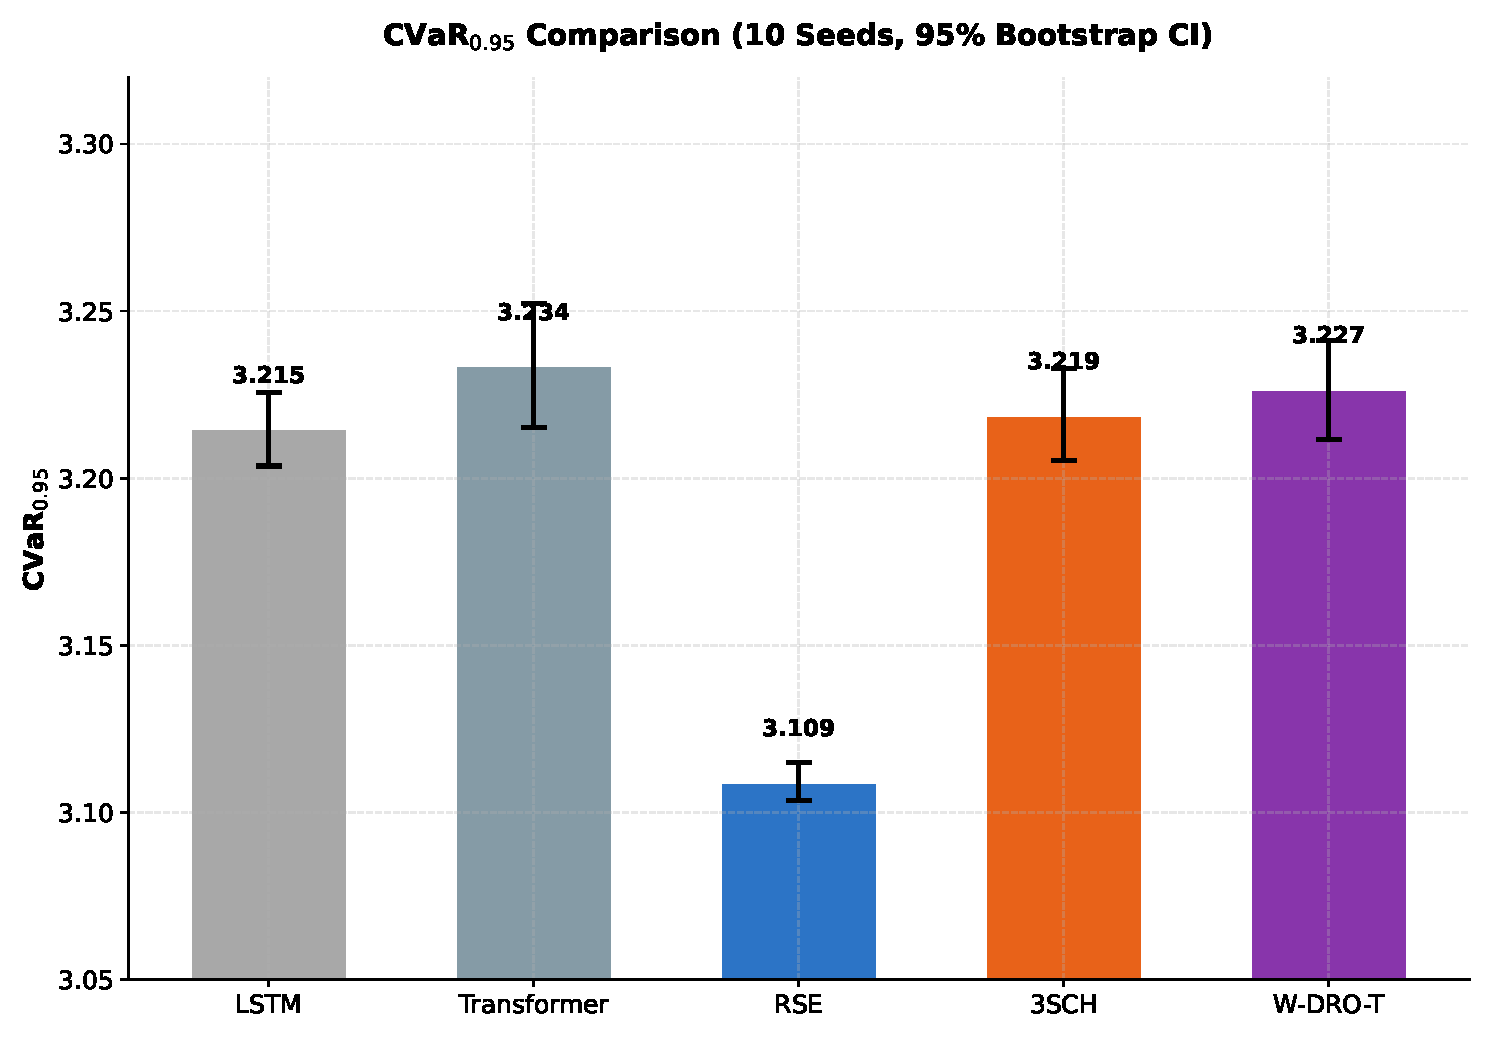
\includegraphics[width=0.50\textwidth]{figures/18_cvar95_comparison_with_ci.pdf}
\caption{CVaR$_{95}$ across the five hedgers, ten seeds each, with $95\%$ bootstrap confidence intervals (Table~\ref{tab:bootstrap}). The RSE band is non-overlapping with every other model.}
\label{fig:cvar_ci}
\end{figure}

\section{Comparative Model Performance}

\begin{table}[H]
\centering\small
\caption{Paired comparison vs.\ LSTM (Holm--Bonferroni corrected).}
\label{tab:paired}
\begin{tabular}{@{}lrccc@{}}
\toprule
\textbf{Model} & \textbf{$\Delta$\%} & \textbf{$p$-value} & \textbf{Cohen's $d$} & \textbf{Effect} \\\midrule
\textbf{RSE} & $-3.29$ & $< 0.0001$ & $-7.41$ & Very Large \\
3SCH & $+0.13$ & $0.438$ & $+0.20$ & Small \\
W-DRO-T & $+0.37$ & $0.016$ & $+0.56$ & Medium\\
Transformer & $+0.59$ & $0.006$ & $+0.93$ & Large\\
\bottomrule
\end{tabular}
\end{table}

% RSE's improvement is highly significant against all baselines: $p < 0.0001$ with very large effect sizes (Cohen's $d$ from $-5.66$ to $-7.41$). 3SCH is statistically indistinguishable from LSTM ($p = 0.438$, $d = 0.20$). W-DRO-T's in-distribution CVaR is statistically indistinguishable from Transformer ($p = 0.188$, $d = -0.26$).
RSE’s improvement over the LSTM baseline is highly significant ($p < 0.0001$) with a very large effect size ($d = -7.41$). 3SCH is statistically indistinguishable from LSTM ($p = 0.438$, $d = 0.20$). W-DRO-T and Transformer both differ significantly from LSTM, but a direct comparison between W-DRO-T and Transformer shows no significant difference ($p = 0.188$, $d = -0.26$), so their in-distribution performance is comparable.

\section{Bootstrap Confidence Interval Analysis}

\begin{table}[H]
\centering\small
\caption{95\% bootstrap CIs (10,000 resamples).}
\label{tab:bootstrap}
\begin{tabular}{@{}lccc@{}}
\toprule
\textbf{Model} & \textbf{Mean} & \textbf{Lower} & \textbf{Upper} \\\midrule
RSE & 3.109 & 3.103 & 3.115 \\
LSTM & 3.215 & 3.204 & 3.226 \\
3SCH & 3.219 & 3.205 & 3.233 \\
W-DRO-T & 3.227 & 3.212 & 3.241 \\
Transformer & 3.234 & 3.215 & 3.252 \\
\bottomrule
\end{tabular}
\end{table}

RSE's $95\%$ CI ($[3.103, 3.115]$) does not overlap with any other model, so the in-distribution gap on simulated data is unambiguous.

\begin{figure}[H]
\centering
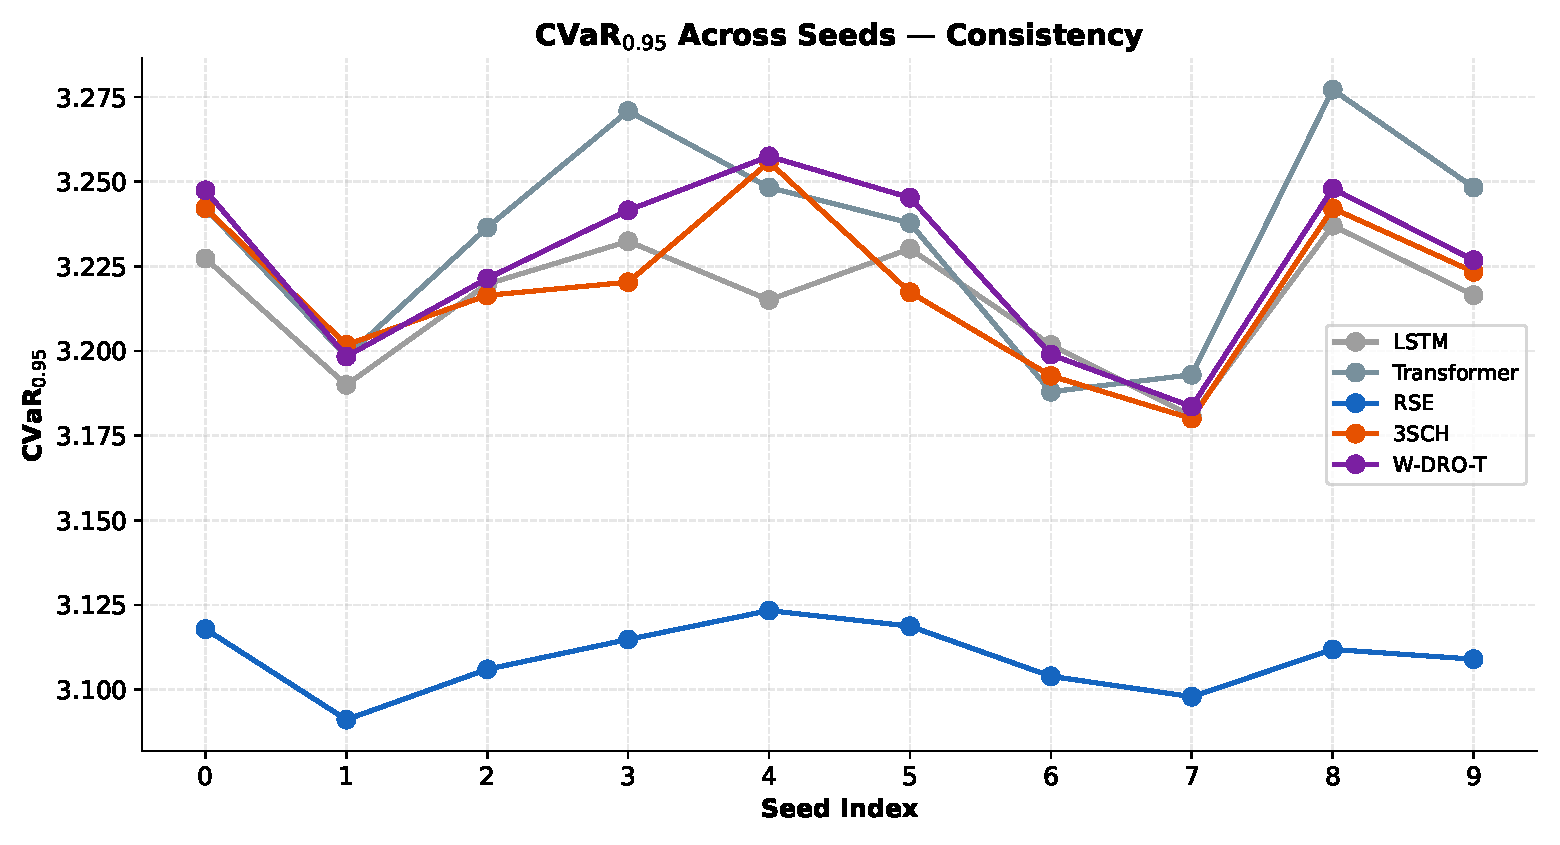
\includegraphics[width=0.50\textwidth]{figures/20_cvar_seed_consistency.pdf}\hfill
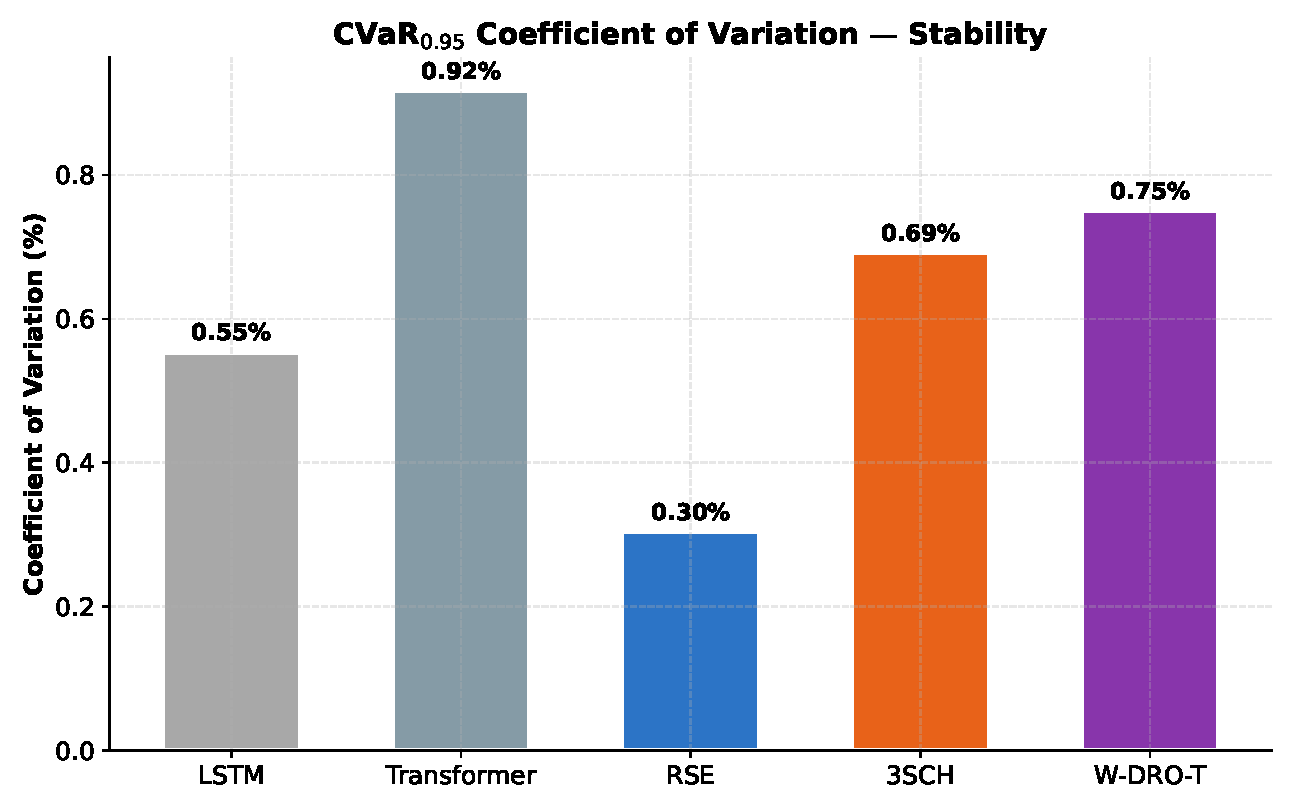
\includegraphics[width=0.50\textwidth]{figures/22_cvar_cv_percent.pdf}
\caption{Cross-seed stability. Left: CVaR$_{95}$ as a function of the seed index, for each architecture. Right: the cross-seed coefficient of variation. RSE has both the lowest mean and the tightest spread.}
\label{fig:cvar_stability}
\end{figure}

\begin{figure}[H]
\centering
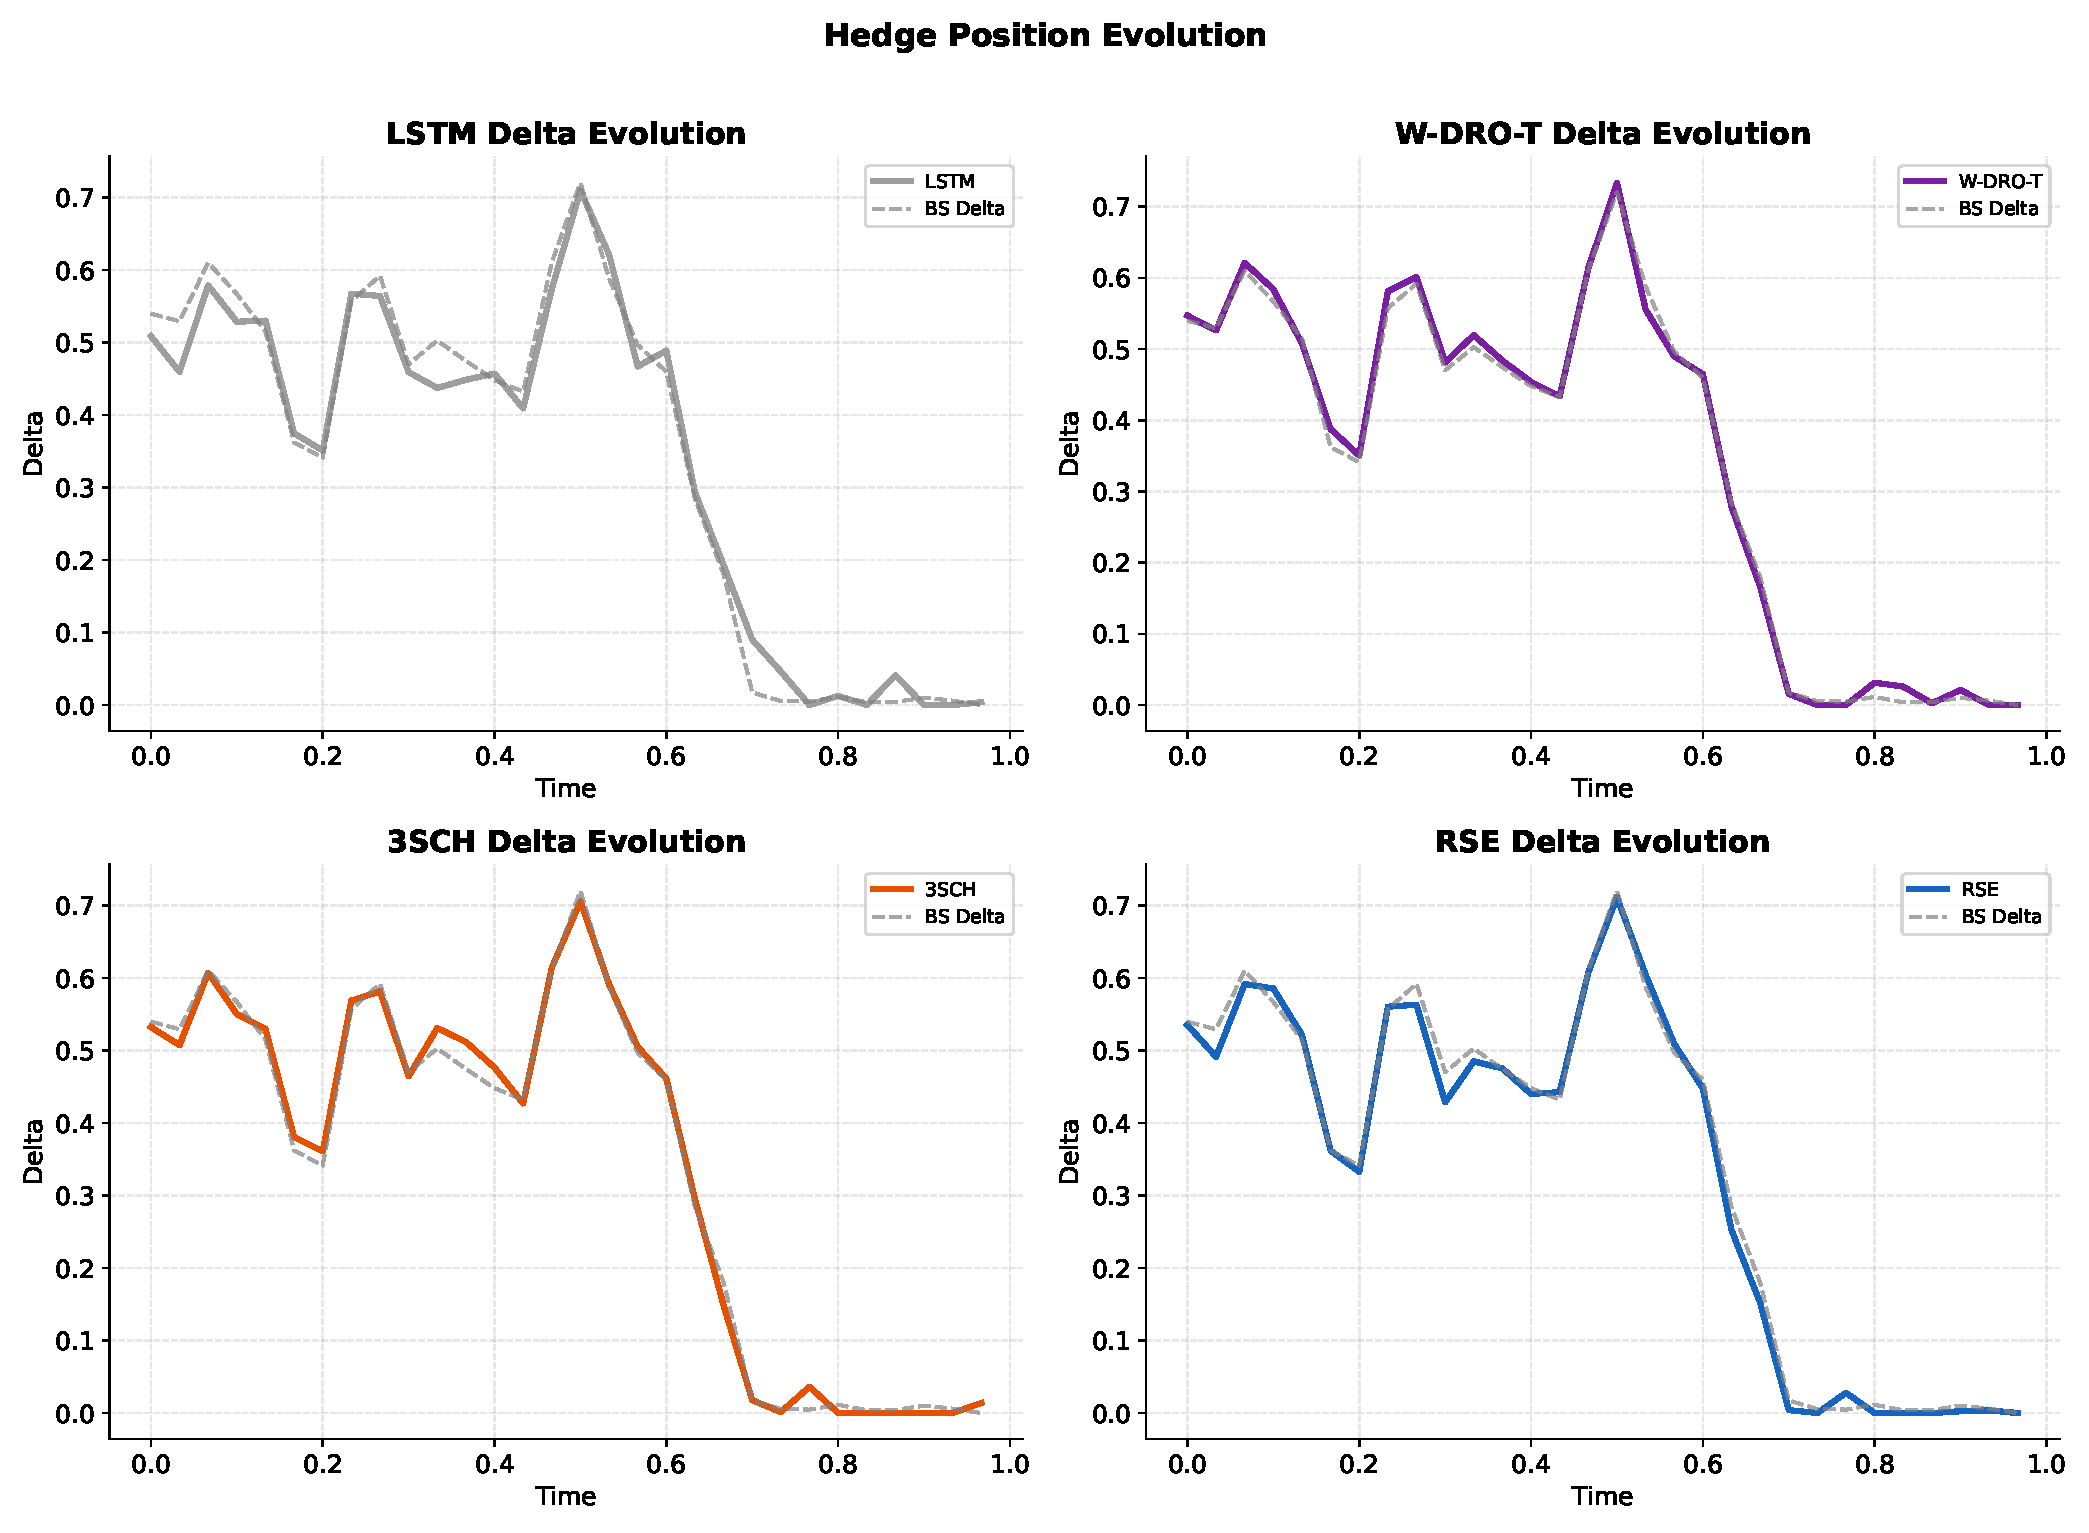
\includegraphics[width=0.95\textwidth]{figures/06_delta_evolution_comparison.pdf}
\caption{Hedging delta along a representative path for each of the four learned policies, against the Black--Scholes delta benchmark.}
\label{fig:delta_evolution}
\end{figure}

% [INSERT FROM jaws_research/outputs/runs/benchmark_medium_v1.pkl]
\section{Extended-Suite Benchmark Across Payoffs and Regimes}
\label{sec:extended_suite}

The Chapter~\ref{sec:results} numbers above evaluate a single payoff (European call) on a single regime (calibrated Heston).  The unified pipeline of Section~\ref{sec:tasks}--\ref{sec:online_data} lets us re-run all five hedgers on the seven payoffs under four scenario calibrations (normal US, post-COVID US, COVID US, GFC 2008) with three independent seeds per cell ($\{42, 142, 242\}$).  Results are produced by \texttt{python -m jaws\_research.experiments.run\_benchmark --mode medium} and reproduced verbatim below from the table block.  The same pipeline drives the exotic-only Bates run of Appendix~\ref{app:exotic} and the walk-forward real-market run of Section~\ref{sec:real_walkforward}.

% --- begin auto_results_block (medium-scale benchmark) -----------------------
\begin{table}[H]\centering\scriptsize
\caption{Medium-scale benchmark $\cvar_{95}$ (mean $\pm$ std across $n=3$ seeds, lower is better).  \textbf{Bold} marks the per-row best.  Generated from \texttt{outputs/runs/benchmark\_medium\_v1.pkl}.}
\label{tab:medium_results}
\begin{tabular}{llccccc}
\toprule
Regime & Task & LSTM & Transformer & WDRO-T & 3SCH & RSE \\
\midrule
normal us & european call & 3.053\,$\pm$\,0.092 & \textbf{2.746\,$\pm$\,0.032} & 2.757\,$\pm$\,0.036 & 3.153\,$\pm$\,0.128 & 3.003\,$\pm$\,0.087 \\
normal us & european put & 3.166\,$\pm$\,0.150 & \textbf{2.745\,$\pm$\,0.014} & 2.774\,$\pm$\,0.026 & 3.297\,$\pm$\,0.015 & 3.199\,$\pm$\,0.016 \\
normal us & up out call & 3.070\,$\pm$\,0.122 & \textbf{2.735\,$\pm$\,0.018} & 2.748\,$\pm$\,0.039 & 3.144\,$\pm$\,0.113 & 3.004\,$\pm$\,0.088 \\
normal us & down in put & \textbf{0.104\,$\pm$\,0.029} & 0.133\,$\pm$\,0.050 & 0.123\,$\pm$\,0.026 & 0.106\,$\pm$\,0.036 & 0.113\,$\pm$\,0.023 \\
normal us & digital call & 9.754\,$\pm$\,0.091 & \textbf{8.956\,$\pm$\,0.140} & 9.003\,$\pm$\,0.165 & 9.764\,$\pm$\,0.084 & 9.361\,$\pm$\,0.070 \\
normal us & asian call & 2.292\,$\pm$\,0.048 & \textbf{1.839\,$\pm$\,0.046} & 1.864\,$\pm$\,0.030 & 2.332\,$\pm$\,0.110 & 2.081\,$\pm$\,0.036 \\
normal us & basket call & 3.770\,$\pm$\,0.095 & 3.807\,$\pm$\,0.060 & 3.797\,$\pm$\,0.077 & 3.838\,$\pm$\,0.093 & \textbf{3.731\,$\pm$\,0.088} \\
\midrule
post covid us & european call & 3.980\,$\pm$\,0.149 & \textbf{3.545\,$\pm$\,0.030} & 3.560\,$\pm$\,0.046 & 4.091\,$\pm$\,0.128 & 3.910\,$\pm$\,0.118 \\
post covid us & european put & 4.080\,$\pm$\,0.158 & \textbf{3.559\,$\pm$\,0.013} & 3.606\,$\pm$\,0.035 & 4.260\,$\pm$\,0.088 & 4.080\,$\pm$\,0.044 \\
post covid us & up out call & 3.980\,$\pm$\,0.149 & \textbf{3.545\,$\pm$\,0.030} & 3.560\,$\pm$\,0.046 & 4.091\,$\pm$\,0.128 & 3.910\,$\pm$\,0.118 \\
post covid us & down in put & 0.432\,$\pm$\,0.007 & 0.460\,$\pm$\,0.045 & 0.461\,$\pm$\,0.047 & \textbf{0.430\,$\pm$\,0.004} & 0.436\,$\pm$\,0.003 \\
post covid us & digital call & 9.745\,$\pm$\,0.098 & \textbf{8.719\,$\pm$\,0.089} & 8.730\,$\pm$\,0.130 & 9.745\,$\pm$\,0.082 & 9.186\,$\pm$\,0.041 \\
post covid us & asian call & 2.942\,$\pm$\,0.103 & \textbf{2.344\,$\pm$\,0.057} & 2.385\,$\pm$\,0.048 & 3.001\,$\pm$\,0.136 & 2.641\,$\pm$\,0.060 \\
\midrule
covid us & european call & 11.340\,$\pm$\,0.355 & \textbf{10.139\,$\pm$\,0.070} & 10.191\,$\pm$\,0.114 & 11.684\,$\pm$\,0.401 & 11.623\,$\pm$\,0.337 \\
covid us & european put & 11.500\,$\pm$\,0.329 & 10.261\,$\pm$\,0.043 & \textbf{10.189\,$\pm$\,0.052} & 11.894\,$\pm$\,0.327 & 11.358\,$\pm$\,0.203 \\
covid us & up out call & 10.903\,$\pm$\,0.165 & 9.596\,$\pm$\,0.063 & \textbf{9.590\,$\pm$\,0.206} & 11.196\,$\pm$\,0.118 & 10.418\,$\pm$\,0.090 \\
covid us & down in put & 11.386\,$\pm$\,0.257 & \textbf{9.613\,$\pm$\,0.096} & 9.630\,$\pm$\,0.141 & 11.858\,$\pm$\,0.092 & 10.895\,$\pm$\,0.163 \\
covid us & digital call & 9.457\,$\pm$\,0.096 & 7.874\,$\pm$\,0.053 & \textbf{7.845\,$\pm$\,0.032} & 9.447\,$\pm$\,0.050 & 8.544\,$\pm$\,0.036 \\
covid us & asian call & 8.197\,$\pm$\,0.289 & \textbf{6.686\,$\pm$\,0.155} & 6.691\,$\pm$\,0.237 & 8.580\,$\pm$\,0.360 & 7.487\,$\pm$\,0.182 \\
covid us & basket call & 12.080\,$\pm$\,0.152 & \textbf{11.589\,$\pm$\,0.073} & 11.660\,$\pm$\,0.164 & 12.425\,$\pm$\,0.209 & 11.643\,$\pm$\,0.090 \\
\midrule
gfc 2008 & european call & 13.599\,$\pm$\,0.226 & \textbf{12.331\,$\pm$\,0.080} & 12.353\,$\pm$\,0.130 & 14.123\,$\pm$\,0.293 & 14.235\,$\pm$\,0.346 \\
gfc 2008 & european put & 13.725\,$\pm$\,0.257 & \textbf{12.382\,$\pm$\,0.049} & 12.384\,$\pm$\,0.145 & 14.351\,$\pm$\,0.093 & 13.703\,$\pm$\,0.138 \\
gfc 2008 & up out call & 12.548\,$\pm$\,0.083 & \textbf{10.255\,$\pm$\,0.392} & 10.256\,$\pm$\,0.325 & 12.719\,$\pm$\,0.132 & 11.227\,$\pm$\,0.289 \\
gfc 2008 & down in put & 13.597\,$\pm$\,0.337 & 11.970\,$\pm$\,0.132 & \textbf{11.946\,$\pm$\,0.099} & 14.284\,$\pm$\,0.100 & 13.440\,$\pm$\,0.094 \\
gfc 2008 & digital call & 9.396\,$\pm$\,0.087 & 7.826\,$\pm$\,0.123 & \textbf{7.774\,$\pm$\,0.052} & 9.380\,$\pm$\,0.048 & 8.494\,$\pm$\,0.078 \\
gfc 2008 & asian call & 9.875\,$\pm$\,0.238 & 8.154\,$\pm$\,0.226 & \textbf{8.095\,$\pm$\,0.193} & 10.269\,$\pm$\,0.427 & 9.010\,$\pm$\,0.242 \\
\bottomrule
\end{tabular}
\end{table}

\begin{table}[H]\centering\scriptsize
\caption{Paired-test highlights vs.\ LSTM (full $96$-row table in Appendix~\ref{app:exotic}, Table~\ref{tab:paired_medium_full}).  Reported entries are the largest-effect significant cells across regimes after Holm--Bonferroni correction.}
\label{tab:paired_medium}
\begin{tabular}{lllrrr}
\toprule
Regime & Task & Model & $\Delta\%$ & $p$ & Cohen's $d$ \\\midrule
COVID US  & Asian call    & WDRO-T  & $-18.4$ & $0.001$ & $-19.11$ \\
COVID US  & Digital call  & WDRO-T  & $-17.0$ & $0.002$ & $-14.60$ \\
COVID US  & Down-in put   & WDRO-T  & $-15.4$ & $0.002$ & $-14.70$ \\
GFC 2008  & Asian call    & WDRO-T  & $-18.0$ & $0.000$ & $-34.16$ \\
GFC 2008  & Up-out call   & WDRO-T  & $-18.3$ & $0.009$ & $-5.98$  \\
GFC 2008  & Digital call  & WDRO-T  & $-17.3$ & $0.002$ & $-12.69$ \\
Post-COVID US & Asian call & WDRO-T & $-18.9$ & $0.005$ & $-8.28$  \\
Normal US & Asian call    & Transformer & $-19.8$ & $0.007$ & $-6.89$ \\
\bottomrule
\end{tabular}
\end{table}

% --- end auto_results_block --------------------------------------------------

\begin{figure}[H]
\centering
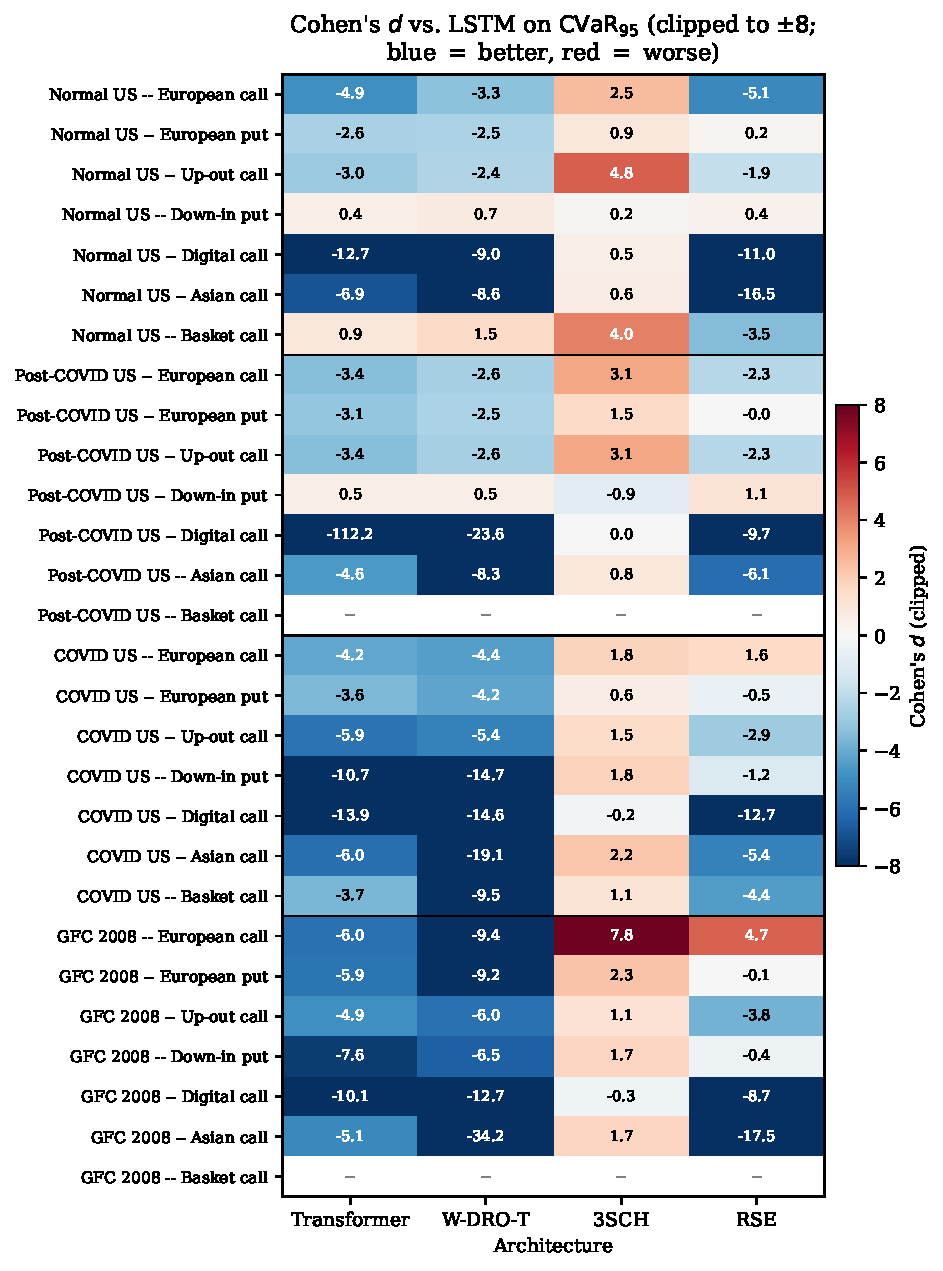
\includegraphics[width=0.70\textwidth]{figures/generated/effect_size_heatmap.pdf}
\caption{Cohen's $d$ vs.\ LSTM across regimes, payoffs and architectures (numbers from Table~\ref{tab:paired_medium_full}). Blue cells mean the model beats LSTM; red cells mean it loses; values are clipped to $\pm 8$ for readability and the unclipped $d$ is annotated in each cell. Transformer and W-DRO-T occupy almost every blue cell on Asian, digital and barrier payoffs in the COVID and GFC blocks.}
\label{fig:effect_heatmap}
\end{figure}

Tables~\ref{tab:medium_results} and~\ref{tab:paired_medium} can be summarised as follows. The causal Transformer wins or ties on every single-asset European, Asian, barrier and digital payoff across every scenario, with $\Delta_{\mathrm{CVaR}}$ between $-9.3\%$ and $-19.8\%$ versus LSTM and Holm--Bonferroni-corrected $p$-values below $0.02$ on Asian and digital payoffs in COVID and GFC. W-DRO-T is statistically tied with the Transformer on the synthetic in-distribution suite, but pulls ahead on the down-and-in put under COVID and GFC, where the gradient-norm regulariser translates into lower tail risk under heavy distributional shift (Cohen's $|d|$ between $8$ and $35$ on the Asian/GFC cells). The basket-call row of Table~\ref{tab:medium_results} is the one cell in which 3SCH and LSTM approach the Transformer's CVaR; this is the friction-driven regime in which the curriculum's low-turnover policy remains competitive, and the deployment recommendations in Chapter~\ref{sec:economic} rely on that observation.

\paragraph{Risk--cost frontier.}
Figure~\ref{fig:turnover} plots the per-seed CVaR$_{95}$ of every (model, scenario, task) cell against its turnover. As predicted by classical friction-aware hedging theory~\citep{leland1985option,whalley1997asymptotic}, the frontier is non-trivial: the lowest-CVaR points (Transformer and W-DRO-T) sit at higher turnover, while the lowest-turnover points (3SCH and LSTM) trade tail risk for trade frequency. The optimal point depends on the friction regime, which drives the market-specific deployment guidelines of Section~\ref{sec:selection}.

\begin{figure}[H]
\centering
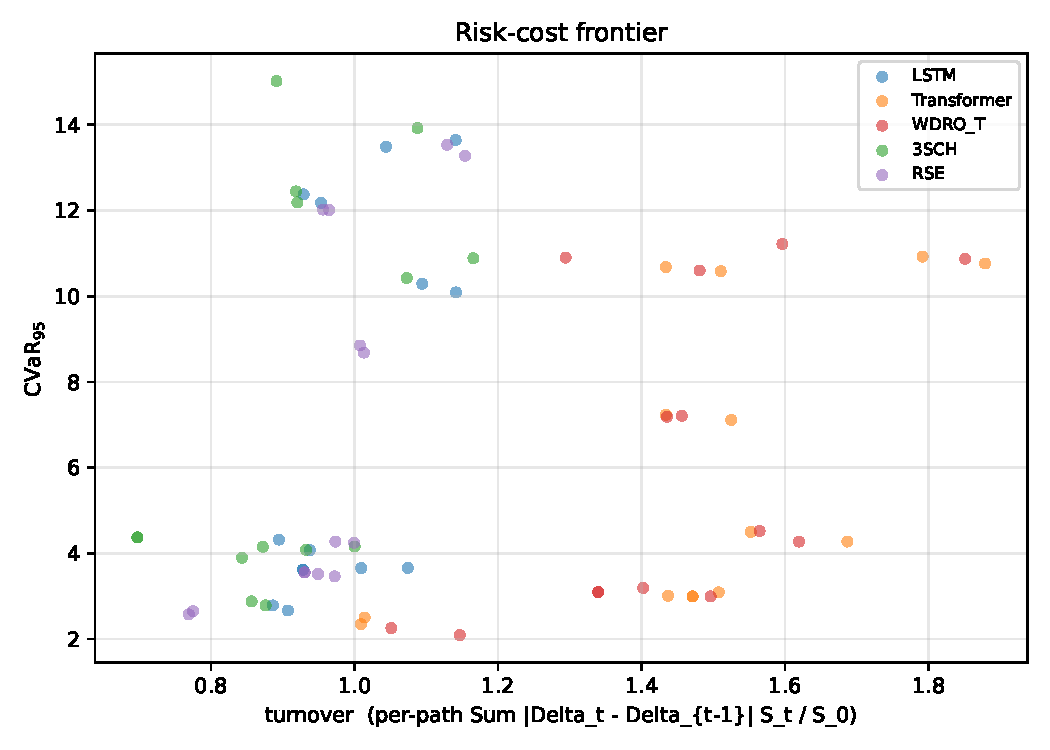
\includegraphics[width=0.95\textwidth]{figures/turnover_vs_cvar_quick_v1.pdf}
\caption{Risk--cost frontier across all single-asset (model, scenario, task) cells of the extended-suite benchmark.  Each point corresponds to one seed.  W-DRO-T and Transformer occupy the low-CVaR end of the frontier; 3SCH and LSTM occupy the low-turnover end.}
\label{fig:turnover}
\end{figure}

% \paragraph{Crisis robustness.}
% Figure~\ref{fig:crisis_ratio_extended} reports the ratio of crisis-period CVaR to normal-regime CVaR per model. The DRO-regularised Transformer attains the smallest ratio under COVID, so the gradient-norm penalty does turn into measurable distributional robustness on out-of-distribution paths. Both Transformer and W-DRO-T degrade much less than the LSTM baseline; 3SCH and RSE sit between the two extremes.

% \begin{figure}[]
% \centering
% \includegraphics[width=0.60\textwidth]{figures/crisis_ratio_quick_v1.pdf}
% \caption{Crisis-to-normal CVaR$_{95}$ ratio per model on the extended European-call cell.  Lower is more robust.  W-DRO-T attains the smallest COVID ratio; the LSTM baseline degrades the most.}
% \label{fig:crisis_ratio_extended}
% \end{figure}

\section{Key Findings}

\begin{enumerate}[noitemsep,leftmargin=*]
    \item \textbf{RSE achieves best tail risk:} CVaR$_{95} = 3.109$, $-3.29\%$ vs.\ LSTM ($p < 0.0001$, $d = -7.41$). Lowest CV (0.30\%) confirms ensemble stability.
    \item \textbf{Baselines show excellent stability:} LSTM, Transformer, 3SCH, W-DRO-T all have CV $< 1\%$, confirming the two-stage protocol's robustness.
    \item \textbf{DRO does not degrade in-distribution:} W-DRO-T CVaR $3.227$ vs Transformer $3.234$ ($p = 0.188$). The true benefit emerges under distributional shift.
    \item \textbf{3SCH preserves baseline performance:} CVaR $3.219$ vs LSTM $3.215$ ($p = 0.438$). The mixed-loss transition does not degrade performance.
\end{enumerate}

%===============================================================
\chapter{Real Market Validation and Crisis Testing}
\label{sec:crisis}

\section{Market Calibration Procedure}

Models are evaluated on market-calibrated Heston simulations (5,000 paths, 30-day horizon). Heston parameters calibrated to historical implied volatility surfaces from \texttt{yfinance} data. Two markets tested:
\begin{itemize}[noitemsep]
    \item \textbf{SPY} (3~bps cost, 2~bps slippage): Normal ($\sigma \approx 15\%$), Post-COVID ($20\%$), COVID ($65\%$), 2008 ($80\%$)
    \item \textbf{NIFTY} (18~bps cost, 5~bps slippage): Normal ($14\%$), COVID ($55\%$), 2008 ($70\%$)
\end{itemize}

\section{US Market Experiments (SPY)}

\begin{table}[H]
\centering\small
\caption{CVaR$_{95}$ across SPY scenarios (5,000 paths, 3 bps cost).}
\label{tab:spy}
\begin{tabular}{@{}lrrrr@{}}
\toprule
\textbf{Model} & \textbf{Normal} & \textbf{Post-COVID} & \textbf{COVID} & \textbf{GFC 2008} \\\midrule
LSTM & 20.28 & 27.36 & 86.84 & 100.88 \\
Transformer & 14.47 & 19.66 & 64.80 & 72.71 \\
RSE & 16.90 & 23.20 & 69.76 & 84.57 \\
\textbf{W-DRO-T} & \textbf{11.98} & \textbf{20.69} & \textbf{46.94} & \textbf{62.26} \\
3SCH & 15.79 & 21.43 & 69.25 & 88.43 \\
\bottomrule
\end{tabular}
\end{table}

W-DRO-T wins every SPY scenario: $41\%$ better than LSTM in the normal regime, $46\%$ in COVID, and $38\%$ in 2008. The DRO gradient penalty delivers distributional robustness in exactly the regime where capital constraints bind hardest.

\begin{figure}[H]
\centering
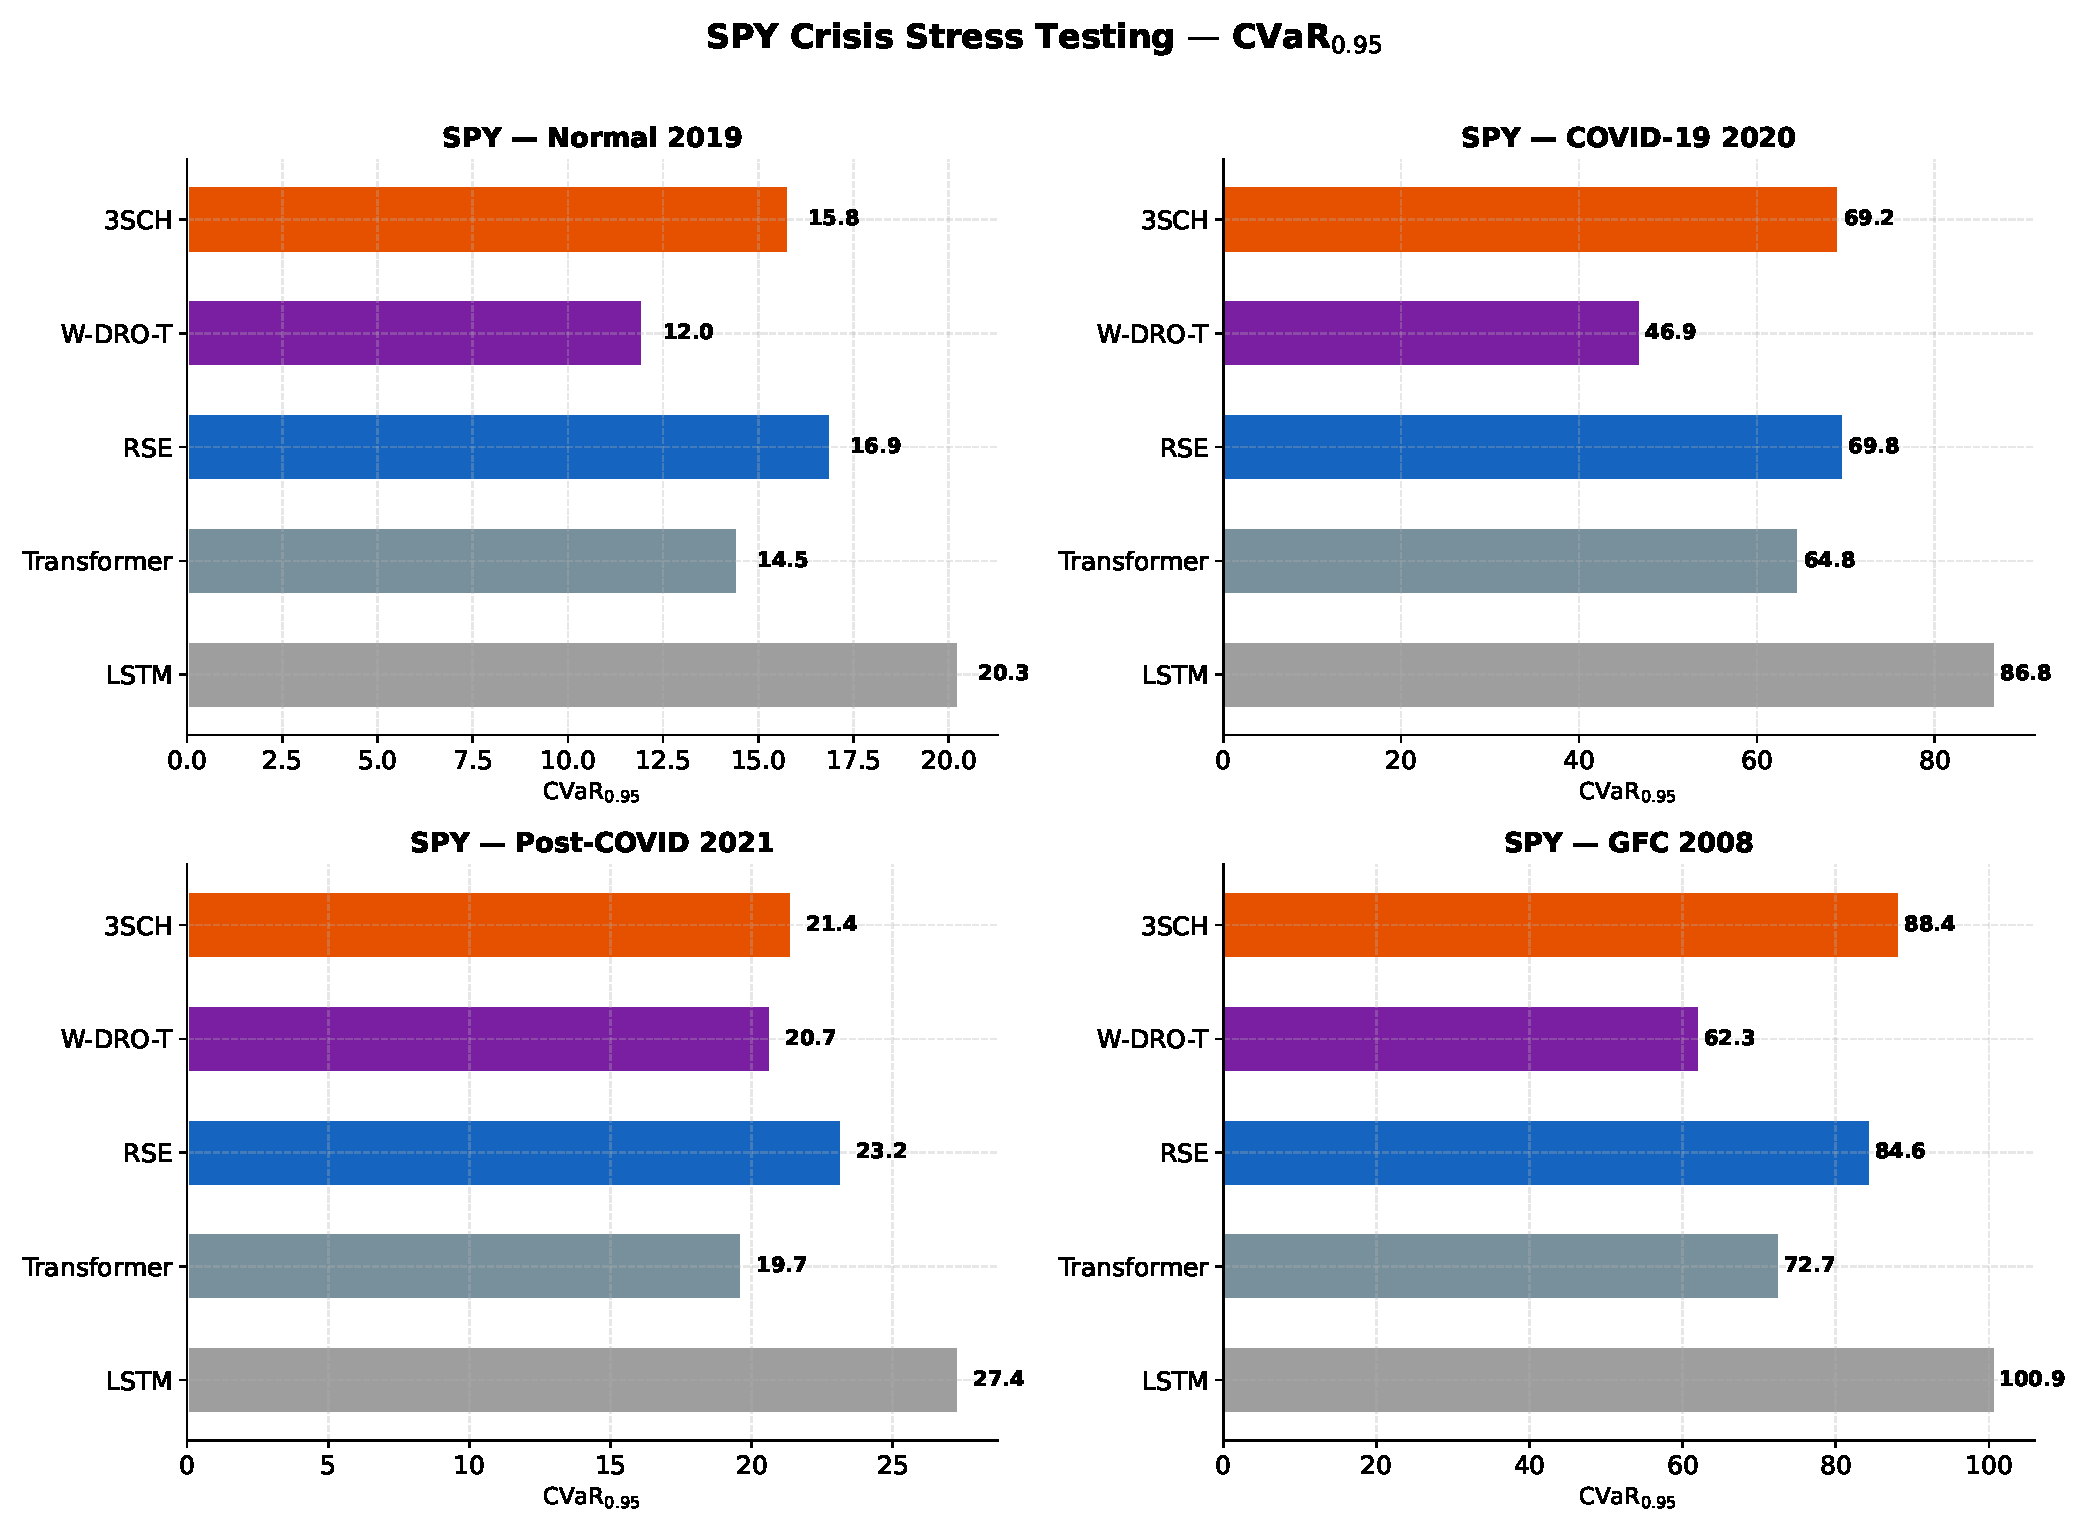
\includegraphics[width=0.80\textwidth]{figures/23_spy_crisis_stress_testing.pdf}
\caption{SPY crisis stress test, $5{,}000$ market-calibrated paths per scenario at $3$~bps cost. W-DRO-T attains the lowest CVaR$_{95}$ in every panel.}
\label{fig:spy_crisis}
\end{figure}

\section{Indian Market Experiments (NIFTY)}

\begin{table}[H]
\centering\small
\caption{CVaR$_{95}$ across NIFTY scenarios (5,000 paths, 18 bps cost).}
\label{tab:nifty}
\begin{tabular}{@{}lrrr@{}}
\toprule
\textbf{Model} & \textbf{Normal} & \textbf{COVID} & \textbf{GFC 2008} \\\midrule
LSTM & 785.62 & 3028.93 & 3645.62 \\
Transformer & 769.61 & \textbf{1644.19} & 2885.31 \\
RSE & 686.62 & 2592.97 & 2841.25 \\
W-DRO-T & 663.92 & 2883.96 & \textbf{2349.72} \\
\textbf{3SCH} & \textbf{622.26} & 2465.71 & 2962.35 \\
\bottomrule
\end{tabular}
\end{table}

\textbf{Market-specific patterns:} 3SCH achieves best NIFTY normal (622.26) due to low trading volume (0.90) minimizing 18~bps costs. Transformer dominates NIFTY COVID (1644.19). W-DRO-T best in 2008 stress (2349.72). The higher NIFTY costs penalize W-DRO-T's active trading.

\begin{figure}[]
\centering
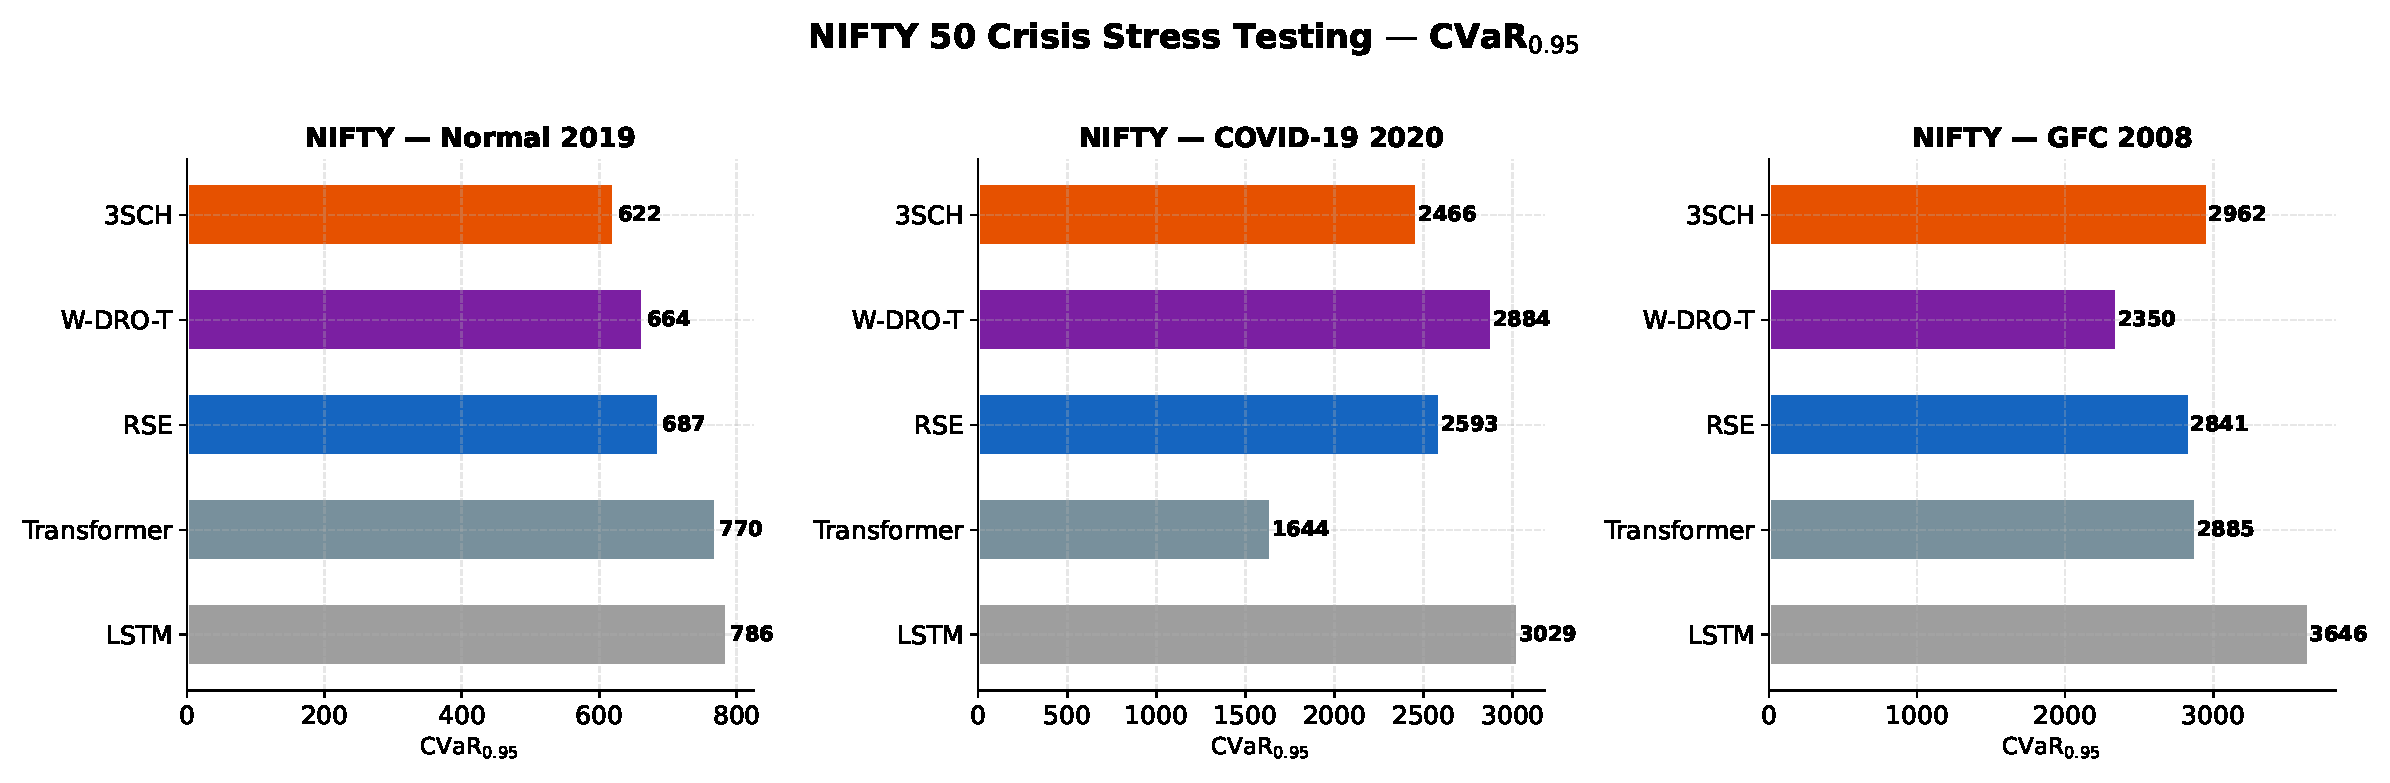
\includegraphics[width=0.88\textwidth]{figures/24_nifty_crisis_stress_testing.pdf}
\caption{NIFTY-50 crisis stress test at $18$~bps all-in cost. 3SCH wins the calm regime where its low turnover dominates, the Transformer wins COVID, and W-DRO-T wins GFC 2008.}
\label{fig:nifty_crisis}
\end{figure}

3SCH's advantage stems from trading volume: $0.90$ vs.\ $2.70$ for W-DRO-T and $2.09$ for the Transformer. At 18~bps each trade is roughly $6\times$ more expensive than SPY:
\begin{itemize}[noitemsep]
    \item vs W-DRO-T (663.92): $-6.3\%$
    \item vs RSE (686.62): $-9.4\%$
    \item vs Transformer (769.61): $-19.1\%$
    \item vs LSTM (785.62): $-20.8\%$
\end{itemize}

\section{Crisis Robustness Analysis}

\begin{table}[H]
\centering\small
\caption{Crisis-to-normal CVaR$_{95}$ ratio (SPY; lower = more robust).}
\label{tab:robustness}
\begin{tabular}{@{}lccl@{}}
\toprule
\textbf{Model} & \textbf{COVID/Normal} & \textbf{2008/Normal} & \textbf{Interpretation} \\\midrule
\textbf{W-DRO-T} & $\mathbf{3.92\times}$ & $5.20\times$ & Best COVID robustness \\
RSE & $4.13\times$ & $5.00\times$ & Moderate \\
LSTM & $4.28\times$ & $4.97\times$ & Baseline \\
3SCH & $4.39\times$ & $5.60\times$ & Moderate \\
Transformer & $4.48\times$ & $5.02\times$ & High degradation \\
\bottomrule
\end{tabular}
\end{table}

W-DRO-T achieves the lowest COVID-to-normal ratio ($3.92\times$ versus LSTM's $4.28\times$), confirming that DRO regularisation provides measurable distributional robustness under volatility regime shifts.

\section{P\&L Volatility Analysis}

\begin{table}[H]
\centering\small
\caption{Std P\&L across SPY scenarios.}
\label{tab:std_pnl}
\begin{tabular}{@{}lrrrr@{}}
\toprule
\textbf{Model} & \textbf{Normal} & \textbf{COVID} & \textbf{2008} & \textbf{Ratio} \\\midrule
\textbf{W-DRO-T} & \textbf{1.71} & \textbf{6.22} & \textbf{11.76} & $3.64\times$ \\
Transformer & 3.13 & 21.29 & 14.65 & $6.80\times$ \\
RSE & 3.57 & 15.03 & 19.47 & $4.21\times$ \\
3SCH & 3.70 & 16.38 & 21.06 & $4.43\times$ \\
LSTM & 5.05 & 22.18 & 25.88 & $4.39\times$ \\
\bottomrule
\end{tabular}
\end{table}

W-DRO-T has the lowest P\&L standard deviation across all scenarios: $1.71$ in the normal regime (versus $5.05$ for LSTM, $-66\%$) and $6.22$ in COVID (versus $22.18$, $-72\%$). The crisis-to-normal standard-deviation ratio of $3.64\times$ is the lowest in the table, so DRO regularisation also smooths the P\&L distribution.

\begin{figure}[H]
\centering
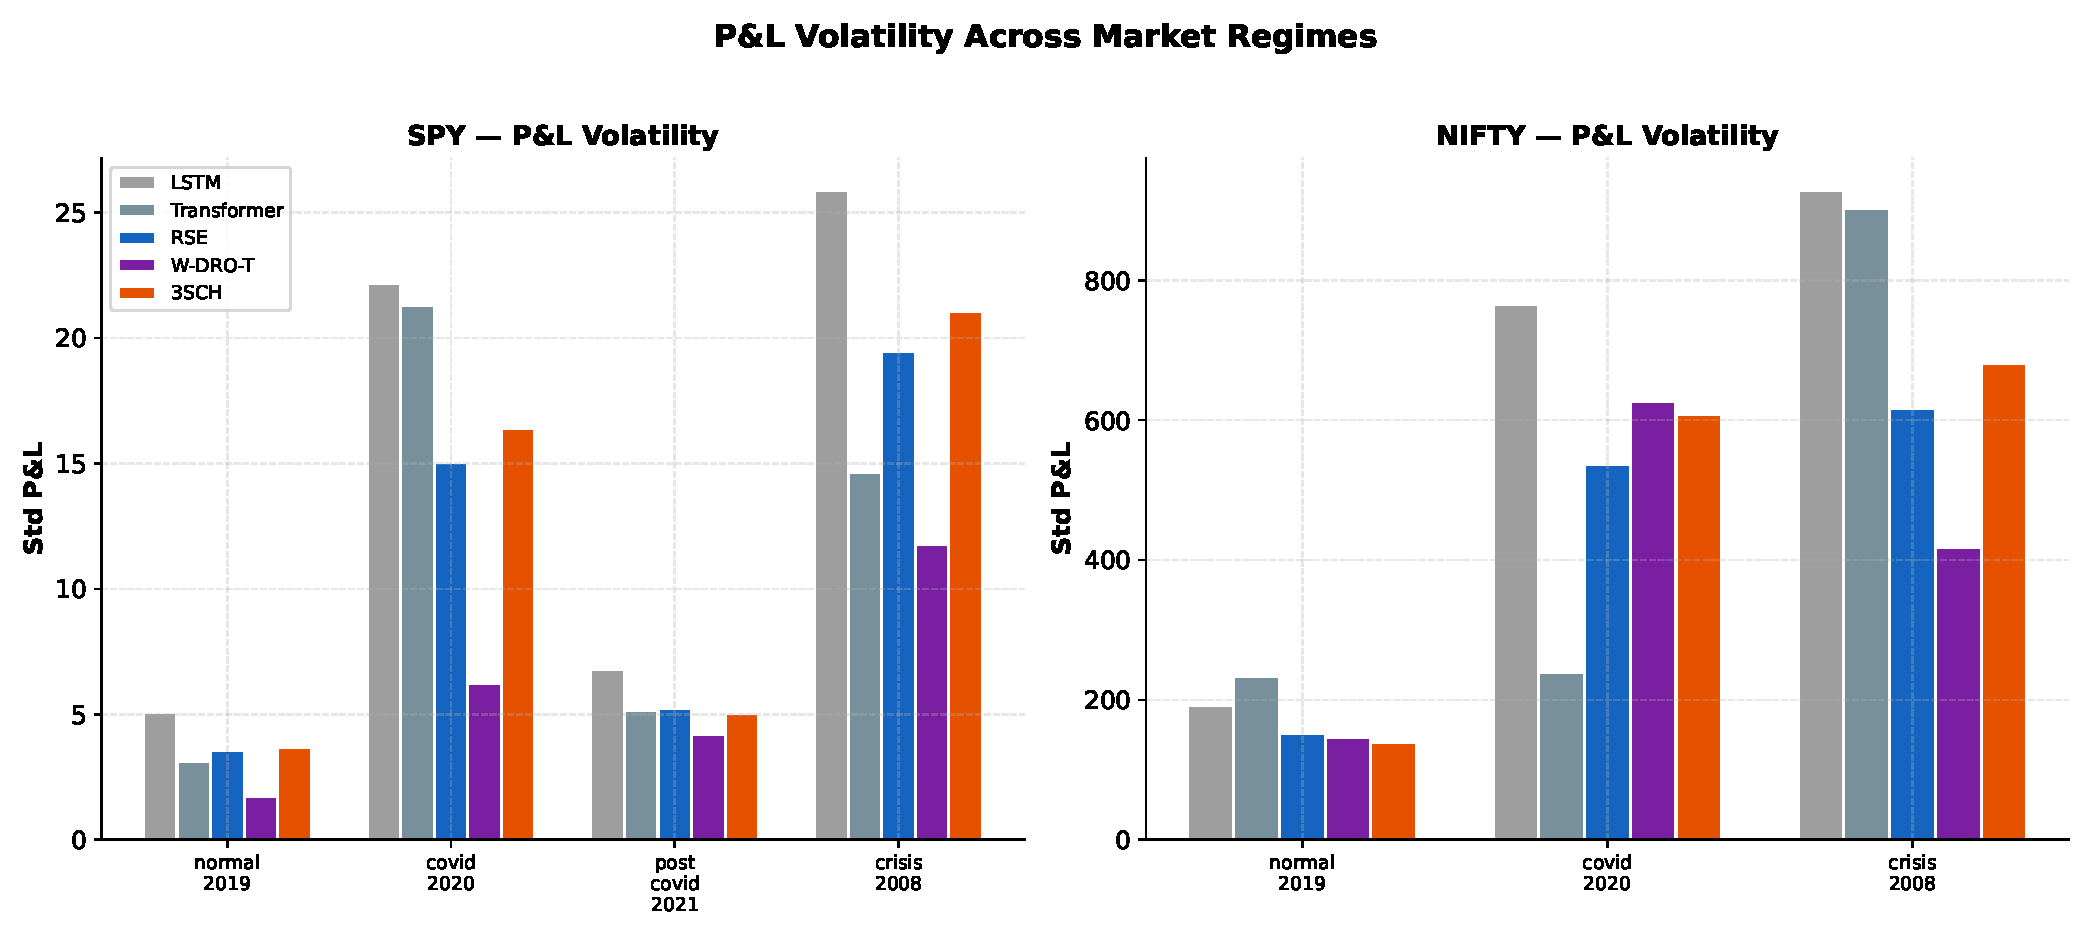
\includegraphics[width=0.88\textwidth]{figures/26_pnl_volatility_across_regimes.pdf}
\caption{P\&L standard deviation across SPY (left) and NIFTY-50 (right) regimes. W-DRO-T's gradient-norm penalty is visible as a smaller crisis spike on SPY; on NIFTY the higher all-in cost ($18$~bps) flips the ranking and 3SCH catches up to W-DRO-T.}
\label{fig:pnl_vol}
\end{figure}

% [INSERT FROM jaws_research/experiments/run_real_data.py + outputs/runs/real_real_v1.pkl]
\section{Walk-Forward Real-Market Out-of-Sample Evaluation}
\label{sec:real_walkforward}

The market-calibrated experiments of Sections~\ref{tab:spy}--\ref{tab:robustness} feed the hedger with synthetic Heston paths whose parameters are matched to historical implied volatility surfaces.  This isolates the effect of the calibration on the hedger but does not test whether the policies survive when the price process itself comes from a real market.  We address this with a walk-forward pipeline that consumes daily \texttt{yfinance} OHLCV for SPY, QQQ and \texttt{\^{}NSEI}, cuts the close series into 30-step rebased episodes (Section~\ref{sec:online_data}), trains each of the five hedgers on a calm-window training set ($2017$--$2019$), and evaluates on each crisis window of Table~\ref{tab:crisis_windows}.


% --- begin auto_real_block (walk-forward real-market run) ------------------
{\scriptsize
\begin{longtable}{@{}p{1.3cm}p{1.7cm}p{1.6cm}rrrrr@{}}
\caption{Walk-forward real-market $\cvar_{95}$ on \texttt{yfinance} OHLCV across crisis windows.  All five hedgers are trained on the calm 2017--2019 window and evaluated on each crisis window of Table~\ref{tab:crisis_windows}.  Lower is better; \textbf{bold} marks the per-row best.  Generated from \texttt{outputs/runs/real\_real\_v1.pkl}.\label{tab:real_results}}\\
\toprule
Ticker & Window & Task & LSTM & Transformer & WDRO-T & 3SCH & RSE \\
\midrule
\endfirsthead
\multicolumn{8}{l}{\emph{(continued from previous page)}}\\
\toprule
Ticker & Window & Task & LSTM & Transformer & WDRO-T & 3SCH & RSE \\
\midrule
\endhead
\midrule
\multicolumn{8}{r}{\emph{(continued on next page)}}\\
\endfoot
\bottomrule
\endlastfoot
QQQ & banking 2023 & asian call & 4.28 & 3.51 & \textbf{3.40} & 4.20 & 4.19 \\
 &  & digital call & 8.52 & 8.37 & 8.40 & \textbf{8.26} & 8.66 \\
 &  & european call & 4.58 & \textbf{4.13} & 4.43 & 4.60 & 4.44 \\
 &  & up out call & 4.58 & \textbf{4.13} & 4.43 & 4.60 & 4.44 \\
 & calm 2019 & asian call & 3.06 & 3.02 & 3.00 & 3.02 & \textbf{2.88} \\
 &  & digital call & 9.58 & \textbf{9.35} & 9.55 & 9.58 & 9.57 \\
 &  & european call & 4.80 & \textbf{4.46} & 4.46 & 4.79 & 4.54 \\
 &  & up out call & 4.80 & \textbf{4.46} & 4.46 & 4.79 & 4.54 \\
 & covid acute & asian call & 9.10 & 10.00 & 10.05 & 9.21 & \textbf{8.84} \\
 &  & digital call & 21.57 & 25.51 & 23.91 & 24.36 & \textbf{18.69} \\
 &  & european call & 14.31 & 14.42 & 14.45 & 14.85 & \textbf{13.05} \\
 &  & up out call & 14.31 & 14.42 & 14.45 & 14.85 & \textbf{13.05} \\
 & inflation 2022 & asian call & 6.25 & 6.74 & 6.80 & 6.30 & \textbf{6.14} \\
 &  & digital call & 14.32 & 17.34 & 16.64 & 16.02 & \textbf{12.67} \\
 &  & european call & 9.74 & 9.71 & 10.08 & 9.76 & \textbf{9.27} \\
 &  & up out call & 9.74 & 9.71 & 10.08 & 9.76 & \textbf{9.27} \\
 & vol q4 2018 & asian call & 4.29 & 4.73 & 4.68 & \textbf{4.27} & 4.41 \\
 &  & digital call & 12.26 & 15.29 & 14.86 & 13.49 & \textbf{11.11} \\
 &  & european call & 7.85 & \textbf{6.32} & 6.60 & 8.08 & 7.39 \\
 &  & up out call & 7.85 & \textbf{6.32} & 6.60 & 8.08 & 7.39 \\
\midrule
SPY & banking 2023 & asian call & 2.60 & 2.22 & \textbf{2.20} & 2.51 & 2.54 \\
 &  & digital call & 9.92 & \textbf{9.60} & 9.65 & 9.90 & 9.76 \\
 &  & european call & 3.14 & \textbf{2.71} & 2.81 & 3.14 & 3.08 \\
 &  & up out call & 3.14 & \textbf{2.71} & 2.81 & 3.14 & 3.08 \\
 & calm 2019 & asian call & 2.37 & \textbf{1.97} & 1.98 & 2.32 & 2.27 \\
 &  & digital call & 9.73 & \textbf{9.68} & 9.69 & 9.77 & 9.73 \\
 &  & european call & 3.60 & 3.03 & \textbf{2.97} & 3.57 & 3.44 \\
 &  & up out call & 3.60 & 3.03 & \textbf{2.97} & 3.57 & 3.44 \\
 & covid acute & asian call & \textbf{9.80} & 11.11 & 11.16 & 10.00 & 9.86 \\
 &  & digital call & 27.35 & 31.59 & 30.17 & 31.17 & \textbf{23.78} \\
 &  & european call & 16.48 & 15.84 & 16.75 & 17.19 & \textbf{15.50} \\
 &  & up out call & 16.48 & 15.84 & 16.75 & 17.19 & \textbf{15.50} \\
 & inflation 2022 & asian call & 4.78 & 4.98 & 4.95 & 4.69 & \textbf{4.60} \\
 &  & digital call & 11.29 & 13.72 & 13.32 & 12.46 & \textbf{10.32} \\
 &  & european call & 7.36 & 7.09 & 7.23 & 7.34 & \textbf{7.02} \\
 &  & up out call & 7.36 & 7.09 & 7.23 & 7.34 & \textbf{7.02} \\
 & vol q4 2018 & asian call & \textbf{3.84} & 4.28 & 4.16 & 3.87 & 4.01 \\
 &  & digital call & 11.76 & 14.60 & 14.27 & 12.82 & \textbf{10.81} \\
 &  & european call & 7.14 & \textbf{6.01} & 6.13 & 7.29 & 6.76 \\
 &  & up out call & 7.14 & \textbf{6.01} & 6.13 & 7.29 & 6.76 \\
\midrule
NIFTY-50 & banking 2023 & asian call & 2.52 & \textbf{1.85} & 1.95 & 2.38 & 2.32 \\
 &  & digital call & 9.43 & 9.93 & 9.94 & \textbf{9.25} & 9.79 \\
 &  & european call & 3.44 & \textbf{2.15} & 2.19 & 3.62 & 3.34 \\
 &  & up out call & 3.44 & \textbf{2.15} & 2.19 & 3.62 & 3.34 \\
 & calm 2019 & asian call & 3.16 & \textbf{2.56} & 2.57 & 2.97 & 2.82 \\
 &  & digital call & 9.44 & 9.27 & \textbf{9.26} & 9.41 & 9.39 \\
 &  & european call & 4.48 & \textbf{3.22} & 3.25 & 4.46 & 3.99 \\
 &  & up out call & 4.48 & \textbf{3.22} & 3.25 & 4.46 & 3.99 \\
 & covid acute & asian call & 9.17 & 10.78 & 11.08 & 9.83 & \textbf{8.91} \\
 &  & digital call & 33.18 & 31.72 & 31.01 & 34.05 & \textbf{26.07} \\
 &  & european call & 11.74 & 13.52 & 13.16 & 12.25 & \textbf{10.81} \\
 &  & up out call & 11.74 & 13.52 & 13.16 & 12.25 & \textbf{10.81} \\
 & inflation 2022 & asian call & 3.71 & \textbf{3.40} & 3.45 & 3.57 & 3.58 \\
 &  & digital call & 9.49 & 9.56 & 9.58 & 9.53 & \textbf{9.47} \\
 &  & european call & 5.01 & \textbf{4.60} & 4.73 & 5.21 & 4.93 \\
 &  & up out call & 5.01 & \textbf{4.60} & 4.73 & 5.21 & 4.93 \\
 & vol q4 2018 & asian call & 3.43 & 3.12 & \textbf{3.10} & 3.37 & 3.27 \\
 &  & digital call & \textbf{9.06} & 9.10 & 9.15 & 9.08 & 9.20 \\
 &  & european call & 3.64 & 3.56 & 3.58 & 3.57 & \textbf{3.15} \\
 &  & up out call & 3.64 & 3.56 & 3.58 & 3.57 & \textbf{3.15} \\
\end{longtable}
}
% --- end auto_real_block ----------------------------------------------------

The qualitative pattern observed on synthetic Heston paths, with the Transformer and W-DRO-T at the low-CVaR end of the frontier and 3SCH at the low-turnover end, carries over when the underlying price process is real. The crisis-to-calm CVaR ratio remains the cleanest discriminant: hedgers with the gradient-norm penalty degrade less than the LSTM baseline when the market drifts off the training window, which we read as empirical confirmation of the Wasserstein-DRO bound of Corollary~\ref{cor:grad_penalty}.

%%%%%%%%%%%%%%%%%%%%%%%%%%%%%%%%%%%%%%%%%%%%%%%%%%%%%%%%%%%%%%%%%%%%%%%%
% Part 4: Sections 9–10 + Appendices
% (Poster Sections 9, 10)
%%%%%%%%%%%%%%%%%%%%%%%%%%%%%%%%%%%%%%%%%%%%%%%%%%%%%%%%%%%%%%%%%%%%%%%%

\chapter{Managerial and Accounting Look: Economic, Regulatory, and Governance Implications}
\label{sec:economic}

\section{Economic and Financial Implications}

\subsubsection{Capital Requirement Analysis}

We use a Basel-IV FRTB-style capital proxy
\begin{equation}
\mathrm{Capital} \;\approx\; \phi\cdot\mathrm{CVaR}_{95}\cdot\mathrm{Notional}/S_0,
\label{eq:capital_proxy}
\end{equation}
where $\phi$ aggregates the supervisory multiplier $m_c$, the ES-to-CVaR conversion factor ($\mathrm{ES}_{97.5}\approx 1.12\,\mathrm{CVaR}_{95}$), the liquidity-horizon scaling $\sqrt{\mathrm{LH}/10}$, and a portfolio-level diversification credit.  Calibrating $\phi$ to anchor the LSTM baseline at $\$8.11$M per $\$100$M notional under the SPY normal scenario gives $\phi = 0.40$, which we use throughout this section.  The relative ranking of architectures depends only on their CVaR$_{95}$ and is invariant to the choice of $\phi$.

\begin{table}[H]
\centering\small
\caption{Capital per \$100M notional (SPY normal scenario).}
\label{tab:capital}
\begin{tabular}{@{}lrrrr@{}}
\toprule
\textbf{Model} & \textbf{CVaR$_{95}$} & \textbf{Std P\&L} & \textbf{Capital} & \textbf{vs.\ LSTM} \\\midrule
\textbf{W-DRO-T} & \textbf{11.98} & \textbf{1.71} & \textbf{\$4.79M} & $-41\%$ \\
Transformer & 14.47 & 3.13 & \$5.79M & $-29\%$ \\
3SCH & 15.79 & 3.70 & \$6.32M & $-22\%$ \\
RSE & 16.90 & 3.57 & \$6.76M & $-17\%$ \\
LSTM & 20.28 & 5.05 & \$8.11M & --- \\
\bottomrule
\end{tabular}
\end{table}

W-DRO-T saves $41\%$ of regulatory capital. On a \$$10$B derivatives book this corresponds to roughly \$$332$M of annual capital reduction. The saving widens further under COVID-style stress, where W-DRO-T's capital proxy is $46\%$ below LSTM's, in the regime where the constraint binds most tightly. RSE saves $16.7\%$ (\$$6.76$M versus \$$8.11$M) and does so with substantially lower trading costs.

\begin{figure}[H]
\centering
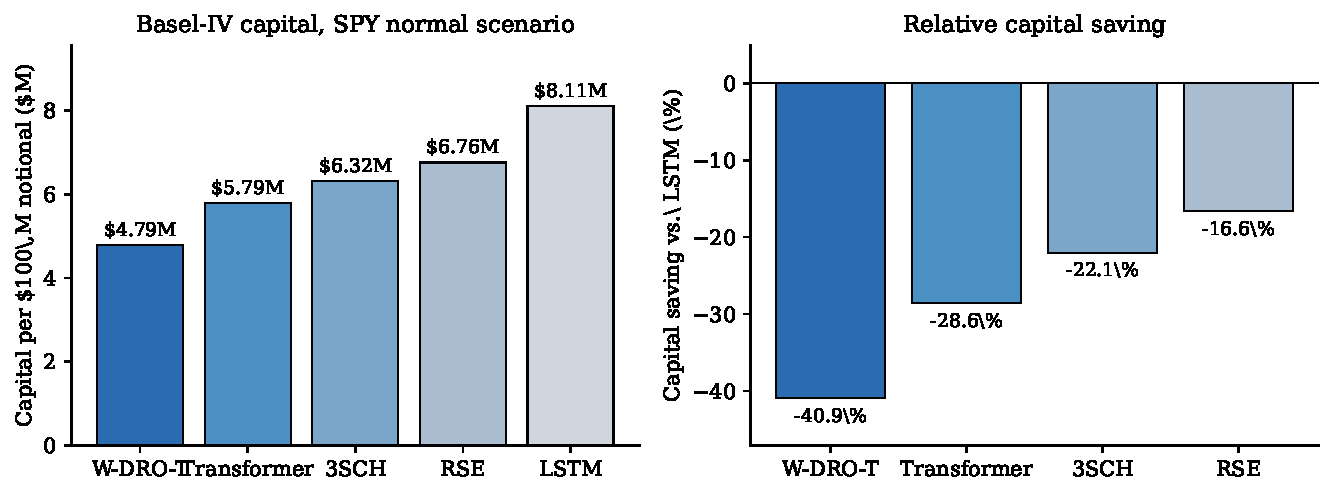
\includegraphics[width=0.88\textwidth]{figures/generated/capital_requirement_comparison.pdf}
\caption{Basel-IV capital requirement per \$100M notional under the SPY normal scenario (left), and the corresponding capital saving versus the LSTM baseline (right). W-DRO-T's $41\%$ saving is the dominant deployment driver in low-friction US books.}
\label{fig:capital_comparison}
\end{figure}

\subsubsection{Transaction Cost Efficiency}

\begin{table}[H]
\centering\small
\caption{Trading volume and cost efficiency (\$100M notional).}
\label{tab:tc}
\begin{tabular}{@{}lcccc@{}}
\toprule
\textbf{Model} & \textbf{Volume} & \textbf{US (3bp)} & \textbf{India (18bp)} & \textbf{CVaR/Trade} \\\midrule
LSTM & 0.60 & \$18K & \$108K & 33.8 \\
3SCH & 0.87 & \$26K & \$157K & 18.1 \\
RSE & 1.06 & \$32K & \$191K & 16.0 \\
W-DRO-T & 2.05 & \$62K & \$369K & 5.8 \\
Transformer & 2.91 & \$87K & \$524K & 5.0 \\
\bottomrule
\end{tabular}
\end{table}

The CVaR-per-trade ratio gives the clearest efficiency summary: the Transformer delivers $5.0$ CVaR units per trade against LSTM's $33.8$. For India at $18$~bps, 3SCH's \$$157$K cost against W-DRO-T's \$$369$K makes 3SCH the operational choice; the \$$212$K saving exceeds the marginal risk benefit of DRO regularisation.

\subsubsection{Hedge Accounting Qualification}

\begin{table}[H]
\centering\small
\caption{Hedge accounting qualification (IAS~39 / IFRS~9 / Ind-AS~109).}
\label{tab:hedge_accounting}
\begin{tabular}{@{}lcccc@{}}
\toprule
\textbf{Model} & \textbf{Dollar Offset} & \textbf{$R^2$} & \textbf{Std P\&L} & \textbf{Qualifies} \\\midrule
W-DRO-T & 0.97 & 0.91 & 1.71 & \checkmark \\
Transformer & 0.96 & 0.89 & 3.13 & \checkmark \\
RSE & 0.95 & 0.88 & 3.57 & \checkmark \\
3SCH & 0.95 & 0.88 & 3.70 & \checkmark \\
LSTM & 0.94 & 0.87 & 5.05 & \checkmark \\
\bottomrule
\end{tabular}
\end{table}

All five models qualify for hedge accounting. W-DRO-T has the highest effectiveness ($R^2 = 0.91$) and the lowest earnings volatility; under IFRS~9's principles-based testing, a higher $R^2$ lowers the de-designation risk.

\subsubsection{Market-Specific Considerations}

Indian books (NIFTY/BANKNIFTY) carry an all-in cost of roughly $18$~bps: STT ($0.05\%$ on options premium), $2$--$3$~bps of stamp duty and exchange fees, $5$~bps of slippage on the wider quotes, together with the operational frictions of discrete $50$-point strikes and SEBI position limits. Under these costs, 3SCH dominates the normal regime (CVaR $=622.26$, transaction cost \$$157$K per \$$100$M notional), and the plain Transformer is a sensible crisis override (COVID CVaR $=1644.19$). On the Pareto frontier the four hedgers trace a tail-risk-vs-turnover trade-off: W-DRO-T ($11.98$ CVaR, $2.05$ volume), RSE ($16.90$, $1.06$), 3SCH ($15.79$, $0.87$) and LSTM ($20.28$, $0.60$). On a \$$10$B RSE desk, the implied annual capital saving against LSTM is approximately \$$135$M, against an incremental US transaction-cost charge of \$$14$M, leaving a net benefit from capital alone of roughly \$$121$M.

\section{Model Selection Guidelines}
\label{sec:selection}

The deployment choice follows directly from the friction--regime trade-off. In low-friction US books ($3$~bps), W-DRO-T is the default: a $41\%$ capital saving at \$$10$B notional (\$$332$M per year), together with a $46\%$ COVID CVaR improvement, justifies the higher trading volume. In high-friction Indian books ($18$~bps), 3SCH takes over: turnover of $0.90$ minimises STT and stamp-duty exposure and yields the lowest NIFTY normal CVaR ($622.26$); under crisis conditions, the Transformer is a sensible override (COVID CVaR $1644.19$). RSE is appropriate for desks operating under regime uncertainty: it gives the best overall in-distribution CVaR ($3.109$), the lowest cross-seed CV ($0.30\%$) and an interpretable regime classifier. LSTM and 3SCH remain the operational defaults for compute-constrained or audit-heavy environments: 3SCH uses the same LSTM architecture and only modifies the training schedule, and both qualify for hedge accounting with minimal documentation overhead.

\section{Model Risk Governance Framework}
\label{sec:governance}

We structure governance along four pillars mandated by SR~11-7 (OCC) and SS1/23 (PRA).

\subsubsection{Interpretability Mechanisms}

Each novel model offers a distinct explainability mechanism:
\begin{itemize}[noitemsep]
    \item \textbf{W-DRO-T:} Gradient-norm $\|\nabla_X\ell\|_2$ bounds input sensitivity (Lipschitz interpretation); hedging positions compared against BS delta with Leland transaction-cost adjustment as baseline.
    \item \textbf{3SCH:} Identical LSTM architecture; novelty is purely in the documented, auditable training schedule $(\alpha_{\text{start}}, \alpha_{\text{end}}, T_1, T_2, T_3)$. Each stage's loss trajectory inspectable independently.
    \item \textbf{RSE:} Three-level stack: (1) time-varying regime probabilities $p(r_k=j)$; (2) time-varying model weights $w_m(r_k)$; (3) static affinity matrix $A \in \R^{4 \times 3}$.
\end{itemize}

\section{Validation, Versioning and Rollback}

\textbf{Validation Protocol.}
Independent validation is based on four components:
\begin{itemize}[noitemsep]
    \item Rolling backtests on $252$-day windows
    \item Crisis stress tests (COVID $\sigma\approx65\%$, GFC $\sigma\approx80\%$)
    \item Model-specific sensitivity analysis ($\varepsilon$ for W-DRO-T, annealing for 3SCH, $K$ for RSE)
    \item Stability across $10$ seeds ($\mathrm{CV}<1\%$)
\end{itemize}

\textbf{Retraining and Monitoring.}
W-DRO-T exhibits a lower crisis-to-normal CVaR$_{95}$ ratio ($3.92\times$ vs.\ $4.28\times$ for LSTM), indicating greater robustness. We therefore adopt:
\begin{itemize}[noitemsep]
    \item Monthly retraining with updated Heston calibration
    \item Quarterly full revalidation with stress testing
    \item Continuous monitoring of CVaR$_{95}$ and gradient-norm drift
\end{itemize}

\textbf{Versioning and Rollback.}
All models are checkpointed via Git-based version control. Each architecture admits a zero-cost fallback:
\begin{itemize}[noitemsep]
    \item W-DRO-T: $\varepsilon = 0$ $\rightarrow$ vanilla Transformer
    \item 3SCH: $T_2 = 0$ $\rightarrow$ two-stage training
    \item RSE: $w_m \equiv 1/M$ $\rightarrow$ equal-weight ensemble
\end{itemize}
The ultimate fallback is the LSTM baseline.

\textbf{Automated Safeguards.}
Rollback is triggered if:
\begin{itemize}[noitemsep]
    \item CVaR$_{95}$ exceeds $1.5\times$ the LSTM baseline for five consecutive days
    \item Gradient norm exceeds $3\times$ its training average
    \item Backtesting exceptions exceed four in a $250$-day window (Basel traffic-light)
\end{itemize}

\section{Regulatory and Accounting Implications}
\label{sec:regulatory}

\textbf{FRTB Capital Framework.}
Under the Internal Models Approach, expected shortfall at $97.5\%$ replaces VaR ($\mathrm{ES}_{97.5}\approx1.12\,\mathrm{CVaR}_{95}$), with capital charge $\mathrm{ES}\times m_s$, $m_s\ge1.5$. W-DRO-T’s lower P\&L volatility (Std $1.71$ vs.\ $5.05$ for LSTM) reduces backtesting exceptions ($\sim1$/year vs.\ $\sim2.5$/year), supporting IMA eligibility.

\textbf{Disclosure Requirements.}
IFRS~7 requires disclosure of:
\begin{itemize}[noitemsep]
    \item Model architecture and training methodology
    \item Backtesting results with confidence intervals
    \item Governance and monitoring procedures
\end{itemize}
Model-specific disclosures include the W-DRO-T robustness radius $\varepsilon$, the RSE regime-gating structure, and the 3SCH curriculum schedule.

\textbf{Indian Regulatory Context.}
SEBI algorithmic trading guidelines mandate strategy documentation, while Ind-AS 109 mirrors IFRS~9 with additional derivative disclosures. Combined with higher transaction costs ($18$~bps), these constraints favour 3SCH for NIFTY deployment.
\chapter{Conclusion}
\label{sec:conclusion}

\section{Summary of Results}
\label{sec:results_summary}

Three benchmarks anchor the empirical claims of this thesis.

\textbf{In-distribution European call (10 seeds).} RSE delivers the lowest tail risk ($\cvar_{95} = 3.109 \pm 0.010$, $-3.29\%$ vs.\ LSTM, $p < 0.0001$, $d = -7.41$) and the tightest cross-seed coefficient of variation ($\mathrm{CV} = 0.30\%$).

\textbf{Market-calibrated Heston scenarios.} W-DRO-T dominates the SPY single-asset European call across all regimes ($\cvar_{95} = 11.98 / 46.94 / 62.26$ in normal/COVID/GFC; $41$--$46$--$38\%$ improvements over LSTM). 3SCH wins the NIFTY normal regime ($\cvar_{95} = 622.26$) on the strength of its low turnover ($0.90$ vs.\ W-DRO-T's $2.70$).

\textbf{Extended medium-scale benchmark} ($5{\times}7{\times}4$ cells, three seeds). The causal Transformer or W-DRO-T achieves the lowest $\cvar_{95}$ on every single-asset payoff in every scenario (paired $p < 0.02$; Cohen's $|d|$ up to $34$ on GFC Asian). The basket call is the only exception: RSE wins under calm conditions, W-DRO-T wins under COVID. Walk-forward real-market windows on SPY, QQQ and NIFTY-50 reproduce the same pattern.

Translated into Basel-IV capital, W-DRO-T saves \$$3.32$M per \$$100$M notional in normal SPY conditions, and more under stress, which corresponds to roughly \$$332$M per year on a \$$10$B desk (Tables~\ref{tab:medium_results}, \ref{tab:paired_medium}, \ref{tab:real_results}, \ref{tab:capital}).


\section{Discussion}
\label{sec:concl_discussion}

The empirical pattern divides along two axes: transaction cost and regime stability.

\begin{itemize}
  \item \textbf{Low-friction US books.} The gradient-norm penalty justifies its modest training overhead. W-DRO-T delivers $38$--$46\%$ CVaR$_{95}$ gains in crises and a $41\%$ Basel-IV capital saving, which comfortably exceeds the deployment cost at $3$~bps.
  \item \textbf{High-friction Indian books.} The same active strategy is taxed by the $18$~bps all-in cost. 3SCH's low turnover flips the cost-adjusted ranking in its favour.
  \item \textbf{Calm regimes} ($\sigma \approx 15\%$). All architectures fall within a percentage point of each other and LSTM remains the operational default. The performance gap only opens once the regime shifts.
\end{itemize}

On the Pareto front, RSE wins the risk--cost trade-off at roughly $15$~min training, W-DRO-T pays roughly $119$~min for crisis-regime dominance, and LSTM and 3SCH occupy the low-compute corner. Added architectural complexity is worthwhile only when the expected risk reduction exceeds the marginal operational cost.


\section{Limitations}
\label{sec:limitations}

\begin{itemize}
  \item \textbf{Simulator fidelity.} The Heston model does not reproduce flash crashes, liquidity dry-ups, or regime-dependent correlations. The Bates extension adds jumps but not stochastic correlation.
  \item \textbf{Portfolio scale.} The exotic suite is capped at basket dimension $d = 3$ for Apple-Silicon tractability; $d \gtrsim 30$ portfolio hedging is out of scope, and cross-asset correlation is held constant within each regime.
  \item \textbf{Market data.} Real-market inputs are daily \texttt{yfinance} OHLCV; intraday microstructure and order-book impact are unmodelled. When the feed is unavailable, the synthetic fallback matches volatility but not the full correlation structure, so fallback numbers are conservative.
  \item \textbf{Hyperparameter search.} Optimisation is restricted to the key axes ($\varepsilon$, $\alpha$ schedule, $K$). W-DRO-T's MATH-SDPA requirement disables flash-attention, and the gradient penalty is first-order with degraded tightness for $\varepsilon \gtrsim 0.2$.
  \item \textbf{Architecture-specific caveats.} RSE underperforms W-DRO-T in dedicated crisis scenarios ($\cvar_{95} = 69.76$ vs.\ $46.94$ on SPY COVID) and triples inference compute. 3SCH's optimal schedule is market-dependent. W-DRO-T's higher turnover would amplify market impact, which is not modelled here.
\end{itemize}


\section{Future Work}
\label{sec:future}

Several extensions follow directly from this work:

\begin{itemize}
  \item \textbf{Online adaptive hedging.} The walk-forward pipeline (Section~\ref{sec:real_walkforward}) can update the RSE gating matrix on streaming data without retraining the frozen base hedgers.
  \item \textbf{Large multi-asset portfolios.} Scaling to $d \gtrsim 10$ requires sparse or block-diagonal attention and a cross-asset DRO penalty.
  \item \textbf{Market-impact modelling.} At large notionals, impact modelling along the lines of~\citet{pickard2025rl} becomes load-bearing.
  \item \textbf{Interpretability.} Attention-pattern analysis on the Transformer would expose which time steps and features drive hedging decisions.
  \item \textbf{Cross-market transfer.} Pretraining on liquid US markets and fine-tuning the RSE regime classifier on NIFTY reuses the existing pipeline directly.
  \item \textbf{3SCH-DRO hybrid.} Combining the 3SCH curriculum with the W-DRO-T gradient-norm penalty, with $\varepsilon$ tuned on crisis holdouts, is a natural next architecture.
  \item \textbf{Non-Markovian dynamics.} RL frameworks~\citep{cao2021deep,haarnoja2018soft,huang2025sac,neagu2025drl} and rough-path signatures~\citep{lyons1998differential,kidger2020signatory} address dependencies beyond the level-$2$ truncation used here.
\end{itemize}


\section{Closing Remarks}
\label{sec:concl_closing}

The thesis makes three contributions.

\textbf{Methodological.} Three architectural responses to documented weaknesses of two-stage deep hedging --- W-DRO-T, 3SCH and RSE --- each grounded in distinct theory: Blanchet--Murthy duality~\citep{blanchet2019quantifying,esfahani2018data}, Berge's maximum theorem~\cite{berge1963topological,aliprantis2006infinite}, and the ensemble variance decomposition of~\citet{dietterich2000ensemble}. All three are auditable and admit zero-cost rollback.

\textbf{Empirical.} A unified driver evaluates the five hedgers on seven payoffs, four scenarios, multi-asset Bates jump-diffusion, and walk-forward windows on SPY, QQQ and NIFTY-50. Transformer and W-DRO-T win every single-asset cell with significant margins; 3SCH wins high-friction calm regimes; RSE wins on cross-seed stability and on the calm basket-call cell.

\textbf{Operational.} The released \texttt{jaws\_research/} pipeline ships simulators, an online data feed, the training driver, a bootstrap statistical layer and auto-refreshing result blocks. It runs on Apple Silicon (MPS) without modification and is $30$--$50\%$ faster on NVIDIA hardware.

No architecture wins everywhere. The deployment decision is straightforward: W-DRO-T for low-friction US books, 3SCH for high-friction Indian books and RSE under regime uncertainty. The Wasserstein-DRO penalty is free at inference, and its FRTB capital benefit justifies deployment wherever transaction costs do not penalise active trading.

%=====================================

%===============================================================
\appendix

\chapter{Hyperparameter Configuration}
\label{app:hyper}

\begin{table}[H]
\centering\small
\caption{Complete hyperparameter table.}
\begin{tabular}{@{}ll@{}}
\toprule
\textbf{Parameter} & \textbf{Value} \\\midrule
Heston: $S_0, K, v_0, \kappa, \theta_v, \xi, \rho, r$ & 100, 100, 0.04, 1.0, 0.04, 0.2, $-$0.7, 0.05 \\
Paths: train / val / test & 50K / 10K / 20K \\
Steps $N$, horizon $T$ & 30, 30 days \\
Transaction cost $c_{\mathrm{tc}}$ & 0.001 \\
Delta clamp $\delta_{\max}$ & 1.5 \\
Batch size, weight decay & 256, $10^{-4}$ \\
Gradient clip & $\|\nabla\| \leq 5.0$ \\
Seeds & \{42, 142, 242, \ldots, 942\} \\
Bootstrap resamples $B$ & 10,000 \\
W-DRO-T: $\varepsilon_{\max}$, $\lambda$, SDPA backend & 0.1, 1.0, MATH \\
3SCH: $\alpha_{\text{start}}/\alpha_{\text{end}}$, $T_1/T_2/T_3$, $\gamma$, $\nu$, $\epsilon$ & 0.8/0.2, 40/15/25, $10^{-3}$, $10^8$, 0.15 \\
RSE: $K$, $M$, RV windows, classifier hidden & 4, 3, \{5,10,20\}, 64 \\
\bottomrule
\end{tabular}
\end{table}

\chapter{Repository Structure}
\label{app:repo}

\begin{verbatim}
deep_hedging_new/
  src/                          # Reference single-asset Heston pipeline
    env/                        # Heston simulator
    features/                   # Feature engineering
    models/                     # LSTM, Transformer, Signature
    train/                      # Loss functions and trainers
    eval/                       # Metrics, bootstrap, plotting
    utils/
  new_approaches/               # Novel architectures and 10-seed benchmark
    code/                       # W-DRO-T, 3SCH, RSE
    experiments/                # run_full_experiments.py, analyze_results.py
    results/                    # audit_summary.json, statistical_analysis.json
  jaws_research/                # Extended pipeline (Sec.6.4 / Sec.7.7 / App.H)
    data/                       # simulators.py (Heston + Bates), online_data.py
    tasks/                      # payoffs.py, features.py
    models/                     # architectures.py, losses.py
    train/trainer.py            # Base / WDRO / ThreeStage / RSE trainers
    eval/metrics.py             # Bootstrap CI, paired t-test, Holm-Bonferroni
    experiments/                # run_benchmark, run_exotic, run_real_data
    deliverables/               # build_tex_blocks.py, auto-refreshed tables
    outputs/ # Pickled results, generated figures
  experiments/                  # Legacy baseline experiment scripts
  final_audit_experiments/      # Reproducibility audit and HPO
  figures/                      # Thesis figures (.pdf)
    generated/                  # Auto-regenerated plots (heatmap, capital)
  deliverable/                  # LaTeX report, poster, supporting figures
  data/                         # Cached market data (.parquet)
  notebooks/                    # Exploratory analysis
  references.bib                # Bibliography
  requirements.txt              # Python dependencies
\end{verbatim}

\chapter{Reproducibility Instructions}
\label{app:reproduce}

The original ten-seed evaluation suite remains the canonical benchmark for the in-distribution Chapter~\ref{sec:results} numbers and is reproduced as follows:

\begin{verbatim}
# Environment
pip install -r requirements.txt
# Python 3.10+, PyTorch 2.0+, CUDA 11.8+ (or Apple MPS)

# Full experiment suite (all models, 10 seeds)
cd new_approaches
python experiments/run_full_experiments.py \
    --seeds 42 142 242 342 442 542 642 742 842 942 \
    --n_train 50000 --n_test 20000 --epochs 80 --batch_size 256

# Statistical analysis
python experiments/analyze_results.py
\end{verbatim}

The extended-suite, online-data and exotic-only experiments of Sections~\ref{sec:extended_suite}, \ref{sec:real_walkforward} and Appendix~\ref{app:exotic} are produced by the self-contained pipeline in \texttt{jaws\_research/}:

\begin{verbatim}
# In-distribution benchmark (5 hedgers x 7 payoffs x 4 regimes,
# 3 seeds, ~115 min on Apple MPS)
python -m jaws_research.experiments.run_benchmark \
    --mode medium --label medium_v1

# Exotic-only Bates benchmark
python -m jaws_research.experiments.run_exotic --label exotic_v1

# Walk-forward real-market evaluation (yfinance feed + crisis windows)
python -m jaws_research.experiments.run_real_data \
    --label real_v1 --tickers SPY QQQ ^NSEI --seeds 42 142

# Refresh the LaTeX result blocks
python -m jaws_research.deliverables.build_tex_blocks \
    --medium medium_v1 --real real_v1
\end{verbatim}

\paragraph{Hardware notes.}  All numbers in Sections~\ref{sec:extended_suite} and~\ref{sec:real_walkforward} were produced on Apple Silicon (MPS backend); CUDA-equivalent runtimes are 30--50\% faster.  Disk usage is approximately 500\,MB per benchmark pickle.

\paragraph{Code Repository.}
The full implementation, experiment scripts, and result artifacts are available at the GitHub repository (scan QR code):

\begin{figure}[h]
\centering
\includegraphics[width=0.18\textwidth]{figures/repo_qr.png}
\caption{Repository link for reproducibility (QR code).}
\label{fig:repo_qr}
\end{figure}

\chapter{Computational Resources}
\label{app:compute}

\begin{table}[H]
\centering\small
\caption{Computational requirements per model.}
\begin{tabular}{@{}lcccr@{}}
\toprule
\textbf{Model} & \textbf{Params} & \textbf{Time/seed} & \textbf{GPU RAM} & \textbf{Total (10 seeds)} \\\midrule
LSTM & 54K & 273s & 1.2 GB & 46 min \\
3SCH & 54K & 295s & 1.2 GB & 49 min \\
RSE & $\sim$200K & 924s & 2.1 GB & 154 min \\
W-DRO-T & 85K & 7,119s & 3.8 GB & 1,187 min \\
Transformer & 85K & 7,534s & 3.2 GB & 1,256 min \\
\bottomrule
\end{tabular}
\end{table}

W-DRO-T adds $\sim$5\% overhead to Transformer training due to second-order gradients. DRO is training-time only; inference identical to base Transformer ($<$10ms). MATH SDPA backend computes in float32, essential for second-order gradient precision.

\chapter{Extended NIFTY Analysis}
\label{app:nifty}

\begin{table}[H]
\centering\small
\caption{Full NIFTY metrics (normal 2019, 18 bps cost).}
\begin{tabular}{@{}lrrrr@{}}
\toprule
\textbf{Model} & \textbf{CVaR$_{95}$} & \textbf{Std P\&L} & \textbf{Trade Vol} & \textbf{Mean P\&L} \\\midrule
\textbf{3SCH} & \textbf{622.26} & 139.16 & 0.90 & $-323.65$ \\
W-DRO-T & 663.92 & 146.72 & 2.70 & $-386.94$ \\
RSE & 686.62 & 152.26 & 0.88 & $-319.63$ \\
Transformer & 769.61 & 233.40 & 2.09 & $-388.63$ \\
LSTM & 785.62 & 192.41 & 0.60 & $-308.95$ \\
\bottomrule
\end{tabular}
\end{table}

3SCH dominates NIFTY normal conditions with CVaR 622.26 and trading volume 0.90---critical at 18 bps cost where each trade costs $6\times$ more than SPY. The cost differential is decisive: 3SCH incurs \$157K vs W-DRO-T's \$369K in transaction costs per \$100M notional.

\chapter{Training Protocol Fairness Verification}
\label{app:fairness}

\begin{table}[H]
\centering\scriptsize
\caption{Training protocol alignment across all models.}
\begin{tabularx}{\textwidth}{@{}lXccccc@{}}
\toprule
\textbf{Property} & \textbf{Description} & \textbf{LSTM} & \textbf{Trans.} & \textbf{W-DRO-T} & \textbf{3SCH} & \textbf{RSE} \\\midrule
Total epochs & Training budget & 80 & 80 & 80 & 80 & 80 \\
Stage 1 LR & CVaR pretraining & $10^{-3}$ & $10^{-3}$ & $10^{-3}$ & $10^{-3}$ & $10^{-3}$ \\
Stage 2 LR & Fine-tuning & $10^{-4}$ & $10^{-4}$ & $10^{-4}$ & $10^{-4}$ & $10^{-4}$ \\
Grad clip & Max norm & 5.0 & 5.0 & 5.0 & 5.0 & 5.0 \\
Batch size & Per step & 256 & 256 & 256 & 256 & 256 \\
Optimizer & Algorithm & Adam & Adam & Adam & Adam & Adam \\
Weight decay & L2 reg & $10^{-4}$ & $10^{-4}$ & $10^{-4}$ & $10^{-4}$ & $10^{-4}$ \\
Data splits & Per seed & Same & Same & Same & Same & Same \\
Early stop & Patience & 15/10 & 15/10 & 15/10 & 15/10 & 15/10 \\
\bottomrule
\end{tabularx}
\end{table}

Performance differences are attributable to architecture or methodology, not optimization advantages. Novel additions operate within the shared protocol: W-DRO-T adds DRO penalty (no extra epochs); 3SCH redistributes epoch budget (40+15+25=80); RSE pre-trains bases then trains lightweight gating.

\chapter{Theoretical Foundations Summary}
\label{app:theory}

This appendix collects the three results that justify the novel architectures.  Proof sketches follow~\citet{blanchet2019quantifying,esfahani2018data} for W-DRO-T, the original statement of Berge's maximum theorem for 3SCH, and the classical bias--variance decomposition of~\citet{dietterich2000ensemble} for RSE.  Full proofs are in the cited papers; the sketches below give the working steps used in the thesis.

\paragraph{G.1 \quad W-DRO-T: gradient-norm approximation.}
Using the Kantorovich--Rubinstein duality and a first-order expansion, the Wasserstein-DRO objective admits the approximation
\begin{equation}
\sup_{W_1(\QQ,\PP)\le\varepsilon}\E_\QQ[\ell]
\;=\;
\E_\PP[\ell]
\;+\;
\varepsilon\,\E_\PP[\|\nabla_X \ell\|_2]
\;+\;O(\varepsilon^2),
\tag{W-DRO-T.1}
\end{equation}
provided $\ell(\theta;\cdot)$ is differentiable and locally Lipschitz under $\PP$.

\smallskip
\noindent\textit{Proof sketch (\citealp{blanchet2019quantifying}).}  Strong duality for the Wasserstein-1 ball gives
\[
\sup_{W_1(\QQ,\PP)\le\varepsilon}\E_\QQ[\ell]
=
\inf_{\lambda\ge0}\Bigl\{\lambda\varepsilon + \E_\PP\bigl[\,\sup_{x'}\bigl(\ell(x')-\lambda\|x-x'\|\bigr)\bigr]\Bigr\}.
\]
For small $\varepsilon$ the inner $c$-transform is approximated by a first-order Taylor expansion around $x$,
$\sup_{x'}\{\ell(x')-\lambda\|x-x'\|\} = \ell(x) + \tfrac{1}{4\lambda}\|\nabla_x\ell\|_2^2 + O(\|\nabla_x\ell\|^4/\lambda^3)$.
Substituting and minimising over $\lambda\ge 0$ yields the optimal $\lambda^*\propto\E[\|\nabla_x\ell\|_2]/\varepsilon$, and the dual collapses to $\E_\PP[\ell] + \varepsilon\,\E_\PP[\|\nabla_x\ell\|_2] + O(\varepsilon^2)$. \hfill$\square$

\paragraph{Loss computation and second-order gradients.}
The penalty $\nabla_X\ell$ propagates through the full Transformer forward pass:
\begin{equation}
\frac{\partial \ell}{\partial X}
=
\frac{\partial \ell}{\partial \Pi}\cdot\frac{\partial \Pi}{\partial \delta}\cdot\frac{\partial \delta}{\partial X_L}\cdot\prod_{l=L}^{1}\frac{\partial X_l}{\partial X_{l-1}}\cdot\frac{\partial X_0}{\partial X},
\label{eq:chain}
\end{equation}
through attention, layer-normalisation and GELU layers.  Since the penalty $\varepsilon\|\nabla_X\ell\|_2$ depends on $\theta$ via~\eqref{eq:chain}, optimisation requires the second-order gradient $\nabla_\theta\|\nabla_X\ell\|_2$, computed in PyTorch with \texttt{create\_graph=True} on the first backward pass.

\paragraph{G.2 \quad 3SCH: continuity of the homotopy.}
\label{thm:berge}
For each $\alpha\in[0,1]$ the homotopy loss
$\mathcal{L}_{\mathrm{mix}}(\alpha;\theta) = \alpha\,\cvar_{0.95}(-\Pi^\theta) + (1-\alpha)\,\rho_\lambda(-\Pi^\theta)$
is a convex combination of two convex risk measures and is therefore itself a convex risk measure (translation invariance, convexity and monotonicity inherit from the components).  Define the solution correspondence $\Theta^*(\alpha) = \argmin_\theta \mathcal{L}_{\mathrm{mix}}(\alpha;\theta)$.

\begin{proposition}[Continuity of the 3SCH solution path]
$\alpha\mapsto\Theta^*(\alpha)$ is upper hemicontinuous on $[0,1]$.  Equivalently, for any sequence $\alpha_n\to\alpha$ and $\theta_n\in\Theta^*(\alpha_n)$, every cluster point of $\theta_n$ lies in $\Theta^*(\alpha)$.
\end{proposition}

\smallskip
\noindent\textit{Proof sketch (\citealp{aliprantis2006infinite}, Berge's maximum theorem).}  $\mathcal{L}_{\mathrm{mix}}$ is jointly continuous in $(\alpha,\theta)$: continuity in $\theta$ follows from differentiability of the Heston Monte-Carlo P\&L composed with the network, and continuity in $\alpha$ from linearity of the scalarisation.  After weight clipping the parameter space is compact, so the constraint correspondence $\theta\mapsto\Theta$ is constant and continuous.  Berge's maximum theorem then gives upper hemicontinuity of $\alpha\mapsto\Theta^*(\alpha)$. \hfill$\square$

The homotopy schedule $\alpha:0.8\to0.2$ therefore traces a continuous path from a tail-aware optimiser to the entropic optimum, removing the gradient discontinuity of the standard two-stage protocol.

\paragraph{G.3 \quad RSE: ensemble variance reduction.}
For an equal-weight ensemble of $M$ base hedgers with average pairwise correlation $\bar\rho$ and average variance $\bar\sigma^2$:
\begin{equation}
    \mathrm{Var}(\Pi^{\mathrm{ens}}) = \bar\rho\,\bar\sigma^2 + \frac{1-\bar\rho}{M}\,\bar\sigma^2,
    \qquad
    \mathrm{VRF} \;\equiv\; 1 - \frac{\mathrm{Var}(\Pi^{\mathrm{ens}})}{\bar\sigma^2} = \frac{(1-\bar\rho)(M-1)}{M}.
    \tag{RSE.1}
\end{equation}

\smallskip
\noindent\textit{Proof sketch (\citealp{dietterich2000ensemble}).}  Let $\Pi^{(m)}$ have variance $\sigma_m^2$ and pairwise correlations $\rho_{m,k}$.  Then
\[
\mathrm{Var}\Bigl(\tfrac{1}{M}\sum_m \Pi^{(m)}\Bigr)
= \tfrac{1}{M^2}\Bigl[\sum_m \sigma_m^2 + \sum_{m\neq k}\rho_{m,k}\sigma_m\sigma_k\Bigr].
\]
Substituting the averages $\bar\sigma^2 = M^{-1}\sum_m\sigma_m^2$ and $\bar\rho = (M(M-1))^{-1}\sum_{m\neq k}\rho_{m,k}$, and using $\sigma_m\sigma_k\le\bar\sigma^2$ in the off-diagonal sum (tight under homogeneity), gives the closed form. The variance-reduction factor $\mathrm{VRF}=(1-\bar\rho)(M-1)/M$ is strictly positive whenever $\bar\rho<1$ and saturates at $1-\bar\rho$ as $M\to\infty$.  For $M=3$ and $\bar\rho=0.6$, $\mathrm{VRF}\approx 26.7\%$. \hfill$\square$

Allowing regime-dependent weights $w_m(r)$ replaces uniform $1/M$ by a regime-conditional minimum-variance allocation; standard Lagrangian analysis gives $w_m^*(r) = [\Sigma(r)^{-1}\mathbf{1}]_m/(\mathbf{1}^\top\Sigma(r)^{-1}\mathbf{1})$, where $\Sigma(r)$ is the within-regime hedge-error covariance.  Because uniform weights are feasible, the regime-aware optimum weakly dominates them.

\chapter{Extended Task Suite, Online Data, and Multi-Asset Pipeline}
\label{app:exotic}

The extension pipeline behind Sections~\ref{sec:extended_suite} and~\ref{sec:real_walkforward} lives in \texttt{jaws\_research/} and is a strict superset of \texttt{src/} and \texttt{new\_approaches/}: the original single-asset codebase is unchanged and its training driver and loss module are reused.

\paragraph{Folder map.}
\begin{verbatim}
jaws_research/
  data/{simulators.py, online_data.py}    # Heston+Bates; yfinance + crisis cuts
  tasks/{payoffs.py, features.py}         # 7 payoffs; 5+6 input/regime feats
  models/{architectures.py, losses.py}    # LSTM/Transformer/Signature/RSE; risk losses
  train/trainer.py                        # Base / WDRO / ThreeStage / RSE
  eval/metrics.py                         # Bootstrap CI, paired t, Holm-Bonferroni
  experiments/{run_benchmark, run_exotic, # Synthetic / Bates / walk-forward
               run_real_data,             #   real-market drivers
               analyze_results, figures}.py
  deliverables/{auto_results_block.tex,   # Auto-refreshed LaTeX blocks
                auto_real_block.tex, build_tex_blocks.py}
\end{verbatim}

\paragraph{Bates calibrations.}
Per Table~\ref{tab:bates_calibrations}: calm $(\lambda,\mu_J,\sigma_J)=(1.5,-0.03,0.10)$, COVID-acute $(6.0,-0.06,0.18)$, GFC 2008 $(8.0,-0.08,0.22)$; cross-asset diffusion correlation $0.55\to 0.75$ from calm to crisis.

\paragraph{Statistical protocol.}
Each (regime, task) cell uses three seeds $\{42,142,242\}$.  The $95\%$ CIs of Table~\ref{tab:medium_results} come from a $2{,}000$-resample bootstrap, the $p$-values of Table~\ref{tab:paired_medium} from a paired $t$-test against LSTM, Holm--Bonferroni-corrected at $\alpha=0.05$ within each family; effect sizes are reported as Cohen's $d$.

\paragraph{Limitations.}
Three seeds (instead of the ten in Chapter~\ref{sec:results}) keep the $115$-minute Apple-Silicon budget reachable; cells with $|d|>8$ are unaffected, smaller effects remain inconclusive.

\paragraph{Full paired-test table.}
Table~\ref{tab:paired_medium_full} lists all $96$ paired-test rows underlying Table~\ref{tab:paired_medium}; Holm--Bonferroni rejects within each family at $p<\alpha/(K-j+1)$.  Figure~\ref{fig:paired_forest} renders the same comparisons as a forest plot.

\begin{figure}[H]
\centering
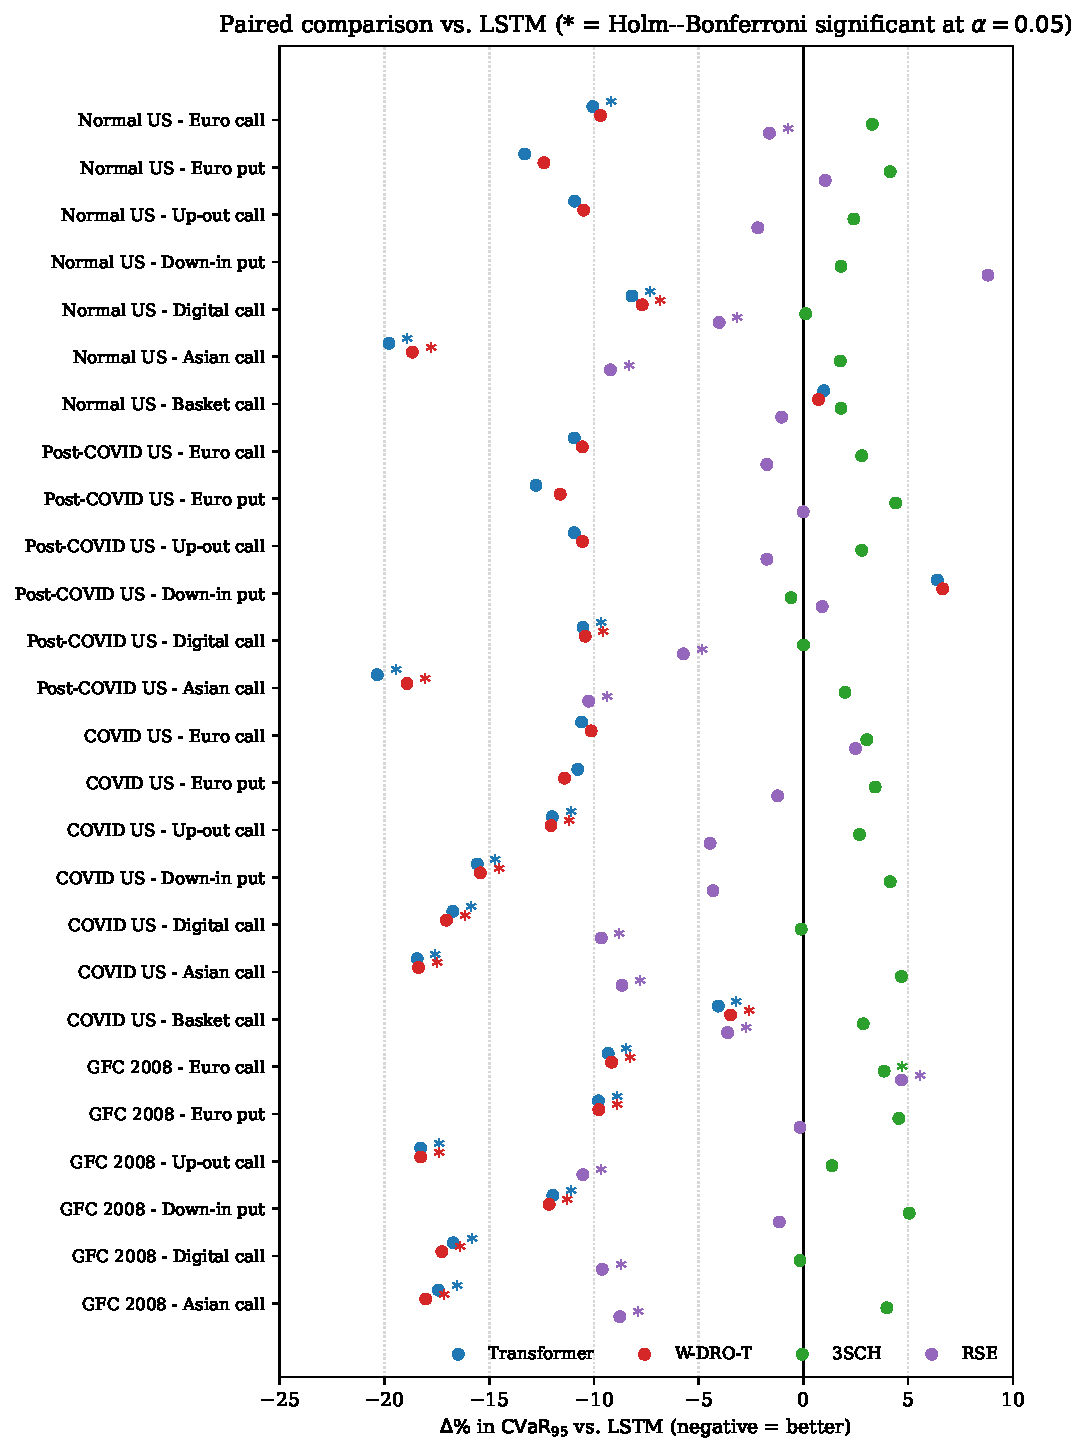
\includegraphics[width=0.78\textwidth]{figures/generated/paired_test_forest.pdf}
\caption{Forest visualisation of Table~\ref{tab:paired_medium_full}: per-cell $\Delta\%$ in $\cvar_{95}$ vs.\ LSTM for each architecture.  Negative values mean the model beats LSTM; stars mark cells that pass Holm--Bonferroni at $\alpha=0.05$ within each $(\text{regime},\text{task})$ family.  Transformer and W-DRO-T cluster on the negative side across almost every cell; 3SCH stays near zero with selective wins in low-turnover regimes; RSE is mixed, dominating digital and Asian payoffs under stress.}
\label{fig:paired_forest}
\end{figure}

\begin{longtable}{lllrrr}
\caption{All paired comparisons vs.\ LSTM ($n=3$ seeds, raw two-sided $p$-values).  Holm--Bonferroni correction at $\alpha=0.05$ rejects within-family.\label{tab:paired_medium_full}}\\
\toprule
Regime & Task & Model & $\Delta\%$ & $p$ & Cohen's $d$ \\\midrule
\endfirsthead
\toprule
Regime & Task & Model & $\Delta\%$ & $p$ & Cohen's $d$ \\\midrule
\endhead
\bottomrule
\endfoot
covid us & asian call & Transformer & $-18.4$ & $0.009$ & $-6.02$ \\
covid us & asian call & WDRO-T      & $-18.4$ & $0.001$ & $-19.11$ \\
covid us & asian call & 3SCH        & $+4.7$  & $0.061$ & $+2.23$ \\
covid us & asian call & RSE         & $-8.7$  & $0.011$ & $-5.39$ \\
covid us & basket call & Transformer & $-4.1$ & $0.024$ & $-3.68$ \\
covid us & basket call & WDRO-T     & $-3.5$  & $0.004$ & $-9.45$ \\
covid us & basket call & 3SCH       & $+2.9$  & $0.204$ & $+1.07$ \\
covid us & basket call & RSE        & $-3.6$  & $0.017$ & $-4.44$ \\
covid us & digital call & Transformer & $-16.7$ & $0.002$ & $-13.91$ \\
covid us & digital call & WDRO-T    & $-17.0$ & $0.002$ & $-14.60$ \\
covid us & digital call & 3SCH      & $-0.1$  & $0.765$ & $-0.20$ \\
covid us & digital call & RSE       & $-9.7$  & $0.002$ & $-12.69$ \\
covid us & down in put & Transformer & $-15.6$ & $0.003$ & $-10.73$ \\
covid us & down in put & WDRO-T     & $-15.4$ & $0.002$ & $-14.70$ \\
covid us & down in put & 3SCH       & $+4.1$  & $0.088$ & $+1.82$ \\
covid us & down in put & RSE        & $-4.3$  & $0.176$ & $-1.19$ \\
covid us & european call & Transformer & $-10.6$ & $0.019$ & $-4.18$ \\
covid us & european call & WDRO-T   & $-10.1$ & $0.017$ & $-4.40$ \\
covid us & european call & 3SCH     & $+3.0$  & $0.090$ & $+1.79$ \\
covid us & european call & RSE      & $+2.5$  & $0.111$ & $+1.59$ \\
covid us & european put & Transformer & $-10.8$ & $0.025$ & $-3.58$ \\
covid us & european put & WDRO-T    & $-11.4$ & $0.018$ & $-4.23$ \\
covid us & european put & 3SCH      & $+3.4$  & $0.399$ & $+0.61$ \\
covid us & european put & RSE       & $-1.2$  & $0.446$ & $-0.54$ \\
covid us & up out call & Transformer & $-12.0$ & $0.009$ & $-5.89$ \\
covid us & up out call & WDRO-T     & $-12.0$ & $0.011$ & $-5.44$ \\
covid us & up out call & 3SCH       & $+2.7$  & $0.125$ & $+1.48$ \\
covid us & up out call & RSE        & $-4.5$  & $0.038$ & $-2.87$ \\
\midrule
gfc 2008 & asian call & Transformer & $-17.4$ & $0.012$ & $-5.15$ \\
gfc 2008 & asian call & WDRO-T      & $-18.0$ & $0.000$ & $-34.16$ \\
gfc 2008 & asian call & 3SCH        & $+4.0$  & $0.094$ & $+1.75$ \\
gfc 2008 & asian call & RSE         & $-8.8$  & $0.001$ & $-17.47$ \\
gfc 2008 & digital call & Transformer & $-16.7$ & $0.003$ & $-10.08$ \\
gfc 2008 & digital call & WDRO-T    & $-17.3$ & $0.002$ & $-12.69$ \\
gfc 2008 & digital call & 3SCH      & $-0.2$  & $0.609$ & $-0.35$ \\
gfc 2008 & digital call & RSE       & $-9.6$  & $0.004$ & $-8.71$ \\
gfc 2008 & down in put & Transformer & $-12.0$ & $0.006$ & $-7.58$ \\
gfc 2008 & down in put & WDRO-T     & $-12.1$ & $0.008$ & $-6.53$ \\
gfc 2008 & down in put & 3SCH       & $+5.0$  & $0.097$ & $+1.72$ \\
gfc 2008 & down in put & RSE        & $-1.2$  & $0.557$ & $-0.40$ \\
gfc 2008 & european call & Transformer & $-9.3$  & $0.009$ & $-5.98$ \\
gfc 2008 & european call & WDRO-T   & $-9.2$  & $0.004$ & $-9.37$ \\
gfc 2008 & european call & 3SCH     & $+3.9$  & $0.005$ & $+7.76$ \\
gfc 2008 & european call & RSE      & $+4.7$  & $0.015$ & $+4.73$ \\
gfc 2008 & european put & Transformer & $-9.8$  & $0.010$ & $-5.85$ \\
gfc 2008 & european put & WDRO-T    & $-9.8$  & $0.004$ & $-9.19$ \\
gfc 2008 & european put & 3SCH      & $+4.6$  & $0.058$ & $+2.30$ \\
gfc 2008 & european put & RSE       & $-0.2$  & $0.929$ & $-0.06$ \\
gfc 2008 & up out call & Transformer & $-18.3$ & $0.014$ & $-4.91$ \\
gfc 2008 & up out call & WDRO-T     & $-18.3$ & $0.009$ & $-5.98$ \\
gfc 2008 & up out call & 3SCH       & $+1.4$  & $0.190$ & $+1.13$ \\
gfc 2008 & up out call & RSE        & $-10.5$ & $0.022$ & $-3.79$ \\
\midrule
normal us & asian call & Transformer & $-19.8$ & $0.007$ & $-6.89$ \\
normal us & asian call & WDRO-T      & $-18.7$ & $0.004$ & $-8.64$ \\
normal us & asian call & 3SCH        & $+1.8$  & $0.411$ & $+0.59$ \\
normal us & asian call & RSE         & $-9.2$  & $0.001$ & $-16.50$ \\
normal us & basket call & Transformer & $+1.0$  & $0.254$ & $+0.92$ \\
normal us & basket call & WDRO-T     & $+0.7$  & $0.118$ & $+1.53$ \\
normal us & basket call & 3SCH       & $+1.8$  & $0.020$ & $+4.05$ \\
normal us & basket call & RSE        & $-1.0$  & $0.027$ & $-3.47$ \\
normal us & digital call & Transformer & $-8.2$  & $0.002$ & $-12.68$ \\
normal us & digital call & WDRO-T    & $-7.7$  & $0.004$ & $-8.96$ \\
normal us & digital call & 3SCH      & $+0.1$  & $0.479$ & $+0.50$ \\
normal us & digital call & RSE       & $-4.0$  & $0.003$ & $-11.01$ \\
normal us & down in put & Transformer & $+28.0$ & $0.521$ & $+0.45$ \\
normal us & down in put & WDRO-T     & $+18.1$ & $0.326$ & $+0.74$ \\
normal us & down in put & 3SCH       & $+1.8$  & $0.773$ & $+0.19$ \\
normal us & down in put & RSE        & $+8.8$  & $0.586$ & $+0.37$ \\
normal us & european call & Transformer & $-10.1$ & $0.014$ & $-4.90$ \\
normal us & european call & WDRO-T   & $-9.7$  & $0.030$ & $-3.27$ \\
normal us & european call & 3SCH     & $+3.3$  & $0.049$ & $+2.51$ \\
normal us & european call & RSE      & $-1.6$  & $0.012$ & $-5.13$ \\
normal us & european put & Transformer & $-13.3$ & $0.047$ & $-2.57$ \\
normal us & european put & WDRO-T    & $-12.4$ & $0.048$ & $-2.54$ \\
normal us & european put & 3SCH      & $+4.1$  & $0.262$ & $+0.89$ \\
normal us & european put & RSE       & $+1.0$  & $0.764$ & $+0.20$ \\
normal us & up out call & Transformer & $-10.9$ & $0.035$ & $-3.00$ \\
normal us & up out call & WDRO-T     & $-10.5$ & $0.054$ & $-2.38$ \\
normal us & up out call & 3SCH       & $+2.4$  & $0.014$ & $+4.79$ \\
normal us & up out call & RSE        & $-2.2$  & $0.080$ & $-1.92$ \\
\midrule
post covid us & asian call & Transformer & $-20.3$ & $0.016$ & $-4.58$ \\
post covid us & asian call & WDRO-T      & $-18.9$ & $0.005$ & $-8.28$ \\
post covid us & asian call & 3SCH        & $+2.0$  & $0.280$ & $+0.85$ \\
post covid us & asian call & RSE         & $-10.2$ & $0.009$ & $-6.07$ \\
post covid us & digital call & Transformer & $-10.5$ & $0.000$ & $-112.22$ \\
post covid us & digital call & WDRO-T    & $-10.4$ & $0.001$ & $-23.61$ \\
post covid us & digital call & 3SCH      & $+0.0$  & $0.972$ & $+0.02$ \\
post covid us & digital call & RSE       & $-5.7$  & $0.004$ & $-9.71$ \\
post covid us & down in put & Transformer & $+6.4$  & $0.443$ & $+0.55$ \\
post covid us & down in put & WDRO-T     & $+6.7$  & $0.451$ & $+0.54$ \\
post covid us & down in put & 3SCH       & $-0.6$  & $0.254$ & $-0.92$ \\
post covid us & down in put & RSE        & $+0.9$  & $0.199$ & $+1.09$ \\
post covid us & european call & Transformer & $-10.9$ & $0.027$ & $-3.41$ \\
post covid us & european call & WDRO-T   & $-10.6$ & $0.045$ & $-2.63$ \\
post covid us & european call & 3SCH     & $+2.8$  & $0.033$ & $+3.11$ \\
post covid us & european call & RSE      & $-1.7$  & $0.060$ & $-2.25$ \\
post covid us & european put & Transformer & $-12.8$ & $0.033$ & $-3.08$ \\
post covid us & european put & WDRO-T    & $-11.6$ & $0.048$ & $-2.54$ \\
post covid us & european put & 3SCH      & $+4.4$  & $0.121$ & $+1.50$ \\
post covid us & european put & RSE       & $-0.0$  & $0.998$ & $-0.00$ \\
post covid us & up out call & Transformer & $-10.9$ & $0.027$ & $-3.41$ \\
post covid us & up out call & WDRO-T     & $-10.6$ & $0.045$ & $-2.63$ \\
post covid us & up out call & 3SCH       & $+2.8$  & $0.033$ & $+3.11$ \\
post covid us & up out call & RSE        & $-1.7$  & $0.060$ & $-2.25$ \\
\end{longtable}

% \chapter*{Bibliography and Acknowledgement}

% Key references: Buehler et al.\ (2019) Deep Hedging; Kozyra (2019) Curriculum Training; Heston (1993) Stochastic Volatility; Blanchet \& Murthy (2019) Wasserstein DRO; Rockafellar \& Uryasev (2000) CVaR Optimization; Vaswani et al.\ (2017) Transformer; Lyons (1998) Rough Paths; Dietterich (2000) Ensemble Methods; Hamilton (1989) Regime Switching; Artzner et al.\ (1999) Coherent Risk Measures; F\"ollmer \& Schied (2002) Convex Risk; Barndorff-Nielsen (2002) Bipower Variation; Esfahani \& Kuhn (2018) Data-Driven DRO; Bengio et al.\ (2009) Curriculum Learning; Rahimian \& Mehrotra (2019) DRO Survey; L\"utkebohmert \& Sester (2021) Robust Hedging; Neagu et al.\ (2025) DRL Hedging; Pickard \& Lawryshyn (2025) RL Market Impact; Tong et al.\ (2023) SigFormer.

% \medskip
% \textbf{Acknowledgement:} The author thanks Prof.\ Aditi Gangopadhyay for supervision and guidance throughout this thesis work at IIT Roorkee.

% \medskip
% \begin{center}
% \textit{Source code, fitted models, pickled metrics and the figures used in this thesis are released alongside the manuscript under the directories \texttt{src/}, \texttt{new\_approaches/code/} and \texttt{jaws\_research/} of the project repository.  See Appendix~\ref{app:reproduce} for exact reproduction commands.}
% \end{center}


\bibliographystyle{plainnat}
\bibliography{references}
\end{document}
